  \documentclass{wissdoc}

% Autor: Roland Bless 1996-2009, bless <at> kit.edu
% ----------------------------------------------------------------
% Diplomarbeit - Hauptdokument
% ----------------------------------------------------------------
%%
%% $Id: diplarb.tex 53 2009-12-10 12:23:37Z bless $
%%
% wissdoc Optionen: draft, relaxed, pdf --> siehe wissdoc.cls
% ------------------------------------------------------------------
% Weitere packages: (Dokumentation dazu durch "latex <package>.dtx")
%\usepackage{bibgerm}
%\usepackage[backend=biber]{biblatex} 
\usepackage{csquotes} 
\usepackage{tabularx}
\usepackage{booktabs}
\usepackage{multirow}
%\usepackage{tocbibind}
\usepackage{siunitx}
\usepackage{xcolor}
\usepackage{textcomp}
\usepackage{listings}
\usepackage{newfloat,caption}
\usepackage{subcaption}
\usepackage{footnote}
\usepackage{rotating}
\usepackage{pgfplots}
\usepackage{pgfplotstable}
\usepackage{url}
\usepackage{boxhandler}
\usepackage{tabu}
\usepackage{amssymb}
%\usepackage{subfig}
%\usepackage{subcaption}
\usepackage{caption}
\usepackage{subcaption}
%\usepackage[plainpages=true]{hyperref}
\usepackage[space]{grffile}
%\usepackage[numbers,sort&compress]{natbib}
\usepackage[backend=bibtex8,natbib=true,hyperref=true,doi=false,url=false]{biblatex}
% \usepackage{varioref}
% \usepackage{verbatim}
\usepackage{float}    %z.B. \floatstyle{ruled}\restylefloat{figure}
\usepackage{todonotes}
%\usepackage[hidelinks]{hyperref}
% \usepackage{subfigure}
% \usepackage{fancybox} % für schattierte,ovale Boxen etc.
% \usepackage{tabularx} % automatische Spaltenbreite
% \usepackage{supertab} % mehrseitige Tabellen
% \usepackage[svnon,svnfoot]{svnver} % SVN Versionsinformation 
%% ---------------- end of usepackages -------------

%\svnversion{$Id: diplarb.tex 53 2009-12-10 12:23:37Z bless $} % In case that you want to include version information in the footer
%\hyphenation{if...-then...}
%% Informationen für die PDF-Datei
\pgfplotsset{compat=newest}

\hypersetup{
%%% styling of link inside pdf
	colorlinks,
  citecolor=black,
  filecolor=black,
  linkcolor=black,
  urlcolor=black,
%%%		
 pdfauthor={FirstName LastName},
 pdftitle={Title of Thesis}
 pdfsubject={Not set},
 pdfkeywords={Not set}
}
\DeclareFloatingEnvironment[fileext=frm,placement={!ht},name=Listing,within=section]{listing}

% Macros, nicht unbedingt notwendig
%%%%%%%%%%%%%%%%%%%%%%%%%%%%%%%%%%%%%%%%%%%%%%%%%%%%%%%%%%
% macros.tex -- einige mehr oder weniger nuetzliche Makros
% Autor: Roland Bless 1998
%%%%%%%%%%%%%%%%%%%%%%%%%%%%%%%%%%%%%%%%%%%%%%%%%%%%%%%%%%
% $Id: macros.tex 33 2007-01-23 09:00:59Z bless $
%%%%%%%%%%%%%%%%%%%%%%%%%%%%%%%%%%%%%%%%%%%%%%%%%%%%%%%%%%


%%%%%%%%%%%%%%%%%%%%%%%
% Kommentare 
%%%%%%%%%%%%%%%%%%%%%%%
\ifnotdraftelse{
\newcommand{\Kommentar}[1]{}
}{\newcommand{\Kommentar}[1]{{\em #1}}}
% Alles innerhalb von \Hide{} oder \ignore{} 
% wird von LaTeX komplett ignoriert (wie ein Kommentar)
\newcommand{\Hide}[1]{}
\let\ignore\Hide

%%%%%%%%%%%%%%%%%%%%%%%%%
% Leere Seite ohne Seitennummer, wird aber gezaehlt
%%%%%%%%%%%%%%%%%%%%%%%%%

\newcommand{\leereseite}{% Leerseite ohne Seitennummer, n�chste Seite rechts (wenn 2-seitig)
 \clearpage{\pagestyle{empty}\cleardoublepage}
}
%%%%%%%%%%%%%%%%%%%%%%%%%%
% Flattersatz rechts und Silbentrennung, Leerraum nach rechts maximal 1cm
%%%%%%%%%%%%%%%%%%%%%%%%%%
\makeatletter
\newcommand{\myraggedright}{%
 \let\\\@centercr\@rightskip 0pt plus 1cm
 \rightskip\@rightskip
  \leftskip\z@skip
  \parindent\z@
  \spaceskip=.3333em
  \xspaceskip=.5em}
\makeatother

\makeatletter
\newcommand{\mynewline}{%
 \@centercr\@rightskip 0pt plus 1cm
}
\makeatother


%%%%%%%%%%%%%%%%%%%%%%%%%%
% F�r Index
%%%%%%%%%%%%%%%%%%%%%%%%%%
\makeatletter
\def\mydotfill{\leavevmode\xleaders\hb@xt@ .44em{\hss.\hss}\hfill\kern\z@}
\makeatother
\def\bold#1{{\bfseries #1}}
\newbox\dbox \setbox\dbox=\hbox to .4em{\hss.\hss} % dot box for leaders
\newskip\rrskipb \rrskipb=.5em plus3em % ragged right space before break
\newskip\rrskipa \rrskipa=-.17em plus -3em minus.11em % ditto, after
\newskip\rlskipa \rlskipa=0pt plus3em % ragged left space after break
\newskip\rlskipb \rlskipb=.33em plus-3em minus.11em % ragged left before break
\newskip\lskip \lskip=3.3\wd\dbox plus1fil minus.3\wd\dbox % for leaders
\newskip \lskipa \lskipa=-2.67em plus -3em minus.11em %after leaders
\mathchardef\rlpen=1000 \mathchardef\leadpen=600
\def\rrspace{\nobreak\hskip\rrskipb\penalty0\hskip\rrskipa}
\def\rlspace{\penalty\rlpen\hskip\rlskipb\vadjust{}\nobreak\hskip\rlskipa}
\let\indexbreak\rlspace
\def\raggedurl{\penalty10000 \hskip.5em plus15em \penalty0 \hskip-.17em plus-15em minus.11em}
\def\raggeditems{\nobreak\hskip\rrskipb \penalty\leadpen \hskip\rrskipa %
\vadjust{}\nobreak\leaders\copy\dbox\hskip\lskip %
\kern3em \penalty\leadpen \hskip\lskipa %
\vadjust{}\nobreak\hskip\rlskipa}
\renewcommand*\see[2]{\rlspace\emph{\seename}~#1} % from makeidx.sty

%%%%%%%%%%%%%%%%%%%%%%%%%%
% Neue Seite rechts, leere linke Seite ohne Headings
%%%%%%%%%%%%%%%%%%%%%%%%%%
\newcommand{\xcleardoublepage}
{{\pagestyle{empty}\cleardoublepage}}

%%%%%%%%%%%%%%%%%%%%%%%%%%
% Tabellenspaltentypen (benoetigt colortbl)
%%%%%%%%%%%%%%%%%%%%%%%%%%
\newcommand{\PBS}[1]{\let\temp=\\#1\let\\=\temp}
\newcolumntype{y}{>{\PBS{\raggedright\hspace{0pt}}}p{1.35cm}}
\newcolumntype{z}{>{\PBS{\raggedright\hspace{0pt}}}p{2.5cm}}
\newcolumntype{q}{>{\PBS{\raggedright\hspace{0pt}}}p{6.5cm}}
\newcolumntype{g}{>{\columncolor[gray]{0.8}}c} % Grau
\newcolumntype{G}{>{\columncolor[gray]{0.9}}c} % helleres Grau

%%%%%%%%%%%%%%%%%%%%%%%%%%
% Anf�hrungszeichen oben und unten
%%%%%%%%%%%%%%%%%%%%%%%%%%
\newcommand{\anf}[1]{"`{#1}"'}

%%%%%%%%%%%%%%%%%%%%%%%%%%
% Tiefstellen von Text
%%%%%%%%%%%%%%%%%%%%%%%%%%
% S\tl{0} setzt die 0 unter das S (ohne Mathemodus!)
% zum Hochstellen gibt es uebrigens \textsuperscript
\makeatletter
\DeclareRobustCommand*\textlowerscript[1]{%
  \@textlowerscript{\selectfont#1}}
\def\@textlowerscript#1{%
  {\m@th\ensuremath{_{\mbox{\fontsize\sf@size\z@#1}}}}}
\let\tl\textlowerscript
\let\ts\textsuperscript
\makeatother

%%%%%%%%%%%%%%%%%%%%%%%%%%
% Gau�-Klammern
%%%%%%%%%%%%%%%%%%%%%%%%%%
\newcommand{\ceil}[1]{\lceil{#1}\rceil}
\newcommand{\floor}[1]{\lfloor{#1}\rfloor}

%%%%%%%%%%%%%%%%%%%%%%%%%%
% Average Operator (analog zu min, max)
%%%%%%%%%%%%%%%%%%%%%%%%%%
\def\avg{\mathop{\mathgroup\symoperators avg}}

%%%%%%%%%%%%%%%%%%%%%%%%%%
% Wortabk�rzungen
%%%%%%%%%%%%%%%%%%%%%%%%%%
\def\zB{z.\,B.\ }
\def\dh{d.\,h.\ }
\def\ua{u.\,a.\ }
\def\su{s.\,u.\ }
\newcommand{\bzw}{bzw.\ }

%%%%%%%%%%%%%%%%%%%%%%%%%%%%%%%%%%%
% Einbinden von Graphiken
%%%%%%%%%%%%%%%%%%%%%%%%%%%%%%%%%%%
% global scaling factor
\def\gsf{0.9}
%% Graphik, 
%% 3 Argumente: Datei, Label, Unterschrift
\newcommand{\Abbildung}[3]{%
\begin{figure}[tbh] %
\centerline{\scalebox{\gsf}{\includegraphics*{#1}}} %
\caption{#3} %
\label{#2} %
\end{figure} %
}
\let\Abb\Abbildung
%% Abbps
%% Graphik, skaliert, Angabe der Position
%% 5 Argumente: Position, Breite (0 bis 1.0), Datei, Label, Unterschrift
\newcommand{\Abbildungps}[5]{%
\begin{figure}[#1]%
\begin{center}
\scalebox{\gsf}{\includegraphics*[width=#2\textwidth]{#3}}%
\caption{#5}%
\label{#4}%
\end{center}
\end{figure}%
}
\let\Abbps\Abbildungps
%% Graphik, Angabe der Position, frei w�hlbares Argument f�r includegraphics
%% 5 Argumente: Position, Optionen, Datei, Label, Unterschrift
\newcommand{\Abbildungpf}[5]{%
\begin{figure}[#1]%
\begin{center}
\scalebox{\gsf}{\includegraphics*[#2]{#3}}%
\caption{#5}%
\label{#4}%
\end{center}
\end{figure}%
}
\let\Abbpf\Abbildungpf

%%
% Anmerkung: \resizebox{x}{y}{box} skaliert die box auf Breite x und H�he y,
%            ist x oder y ein !, dann wird das uspr�ngliche 
%            Seitenverh�ltnis beibehalten.
%            \rescalebox funktioniert �hnlich, nur das dort ein Faktor
%            statt einer Dimension angegeben wird.
%%
% \Abbps{Position}{Breite in Bruchteilen der Textbreite}{Dateiname}{Label}{Bildunterschrift}
%

\newcommand{\refAbb}[1]{%
s.~Abbildung \ref{#1}}

%%%%%%%%%%%%%%%%%%%%
%% end of macros.tex
%%%%%%%%%%%%%%%%%%%%

% Print URLs not in Typewriter Font
\def\UrlFont{\rm}

\newcommand{\specialcell}[2][c]{%
  \begin{tabular}[#1]{@{}c@{}}#2\end{tabular}}

%\newcommand\todo[1]{\textcolor{red}{TODO: #1}}

\newcommand\hlcode[1]{\textcolor{red}{#1}}

\newcommand\citeable[1]{\textcolor{green}{\hl{citeable: #1}}}

\newcolumntype{$}{>{\global\let\currentrowstyle\relax}}
\newcolumntype{^}{>{\currentrowstyle}}
\newcommand{\rowstyle}[1]{\gdef\currentrowstyle{#1}%
  #1\ignorespaces
}

\newif\ifcomment
%\commenttrue %# Show comments


\newcommand{\blankpage}{% Leerseite ohne Seitennummer, nächste Seite rechts
 \clearpage{\pagestyle{empty}\cleardoublepage}
}

%% Einstellungen für das gesamte Dokument

% Trennhilfen
% Wichtig! 
% Im german-paket sind zusätzlich folgende Trennhinweise enthalten:
% "- = zusätzliche Trennstelle
% "| = Vermeidung von Ligaturen und mögliche Trennung (bsp: Schaf"|fell)
% "~ = Bindestrich an dem keine Trennung erlaubt ist (bsp: bergauf und "~ab)
% "= = Bindestrich bei dem Worte vor und dahinter getrennt werden dürfen
% "" = Trennstelle ohne Erzeugung eines Trennstrichs (bsp: und/""oder)

% Trennhinweise fuer Woerter hier beschreiben
\hyphenation{
% Pro-to-koll-in-stan-zen
% Ma-na-ge-ment  Netz-werk-ele-men-ten
% Netz-werk Netz-werk-re-ser-vie-rung
% Netz-werk-adap-ter Fein-ju-stier-ung
% Da-ten-strom-spe-zi-fi-ka-tion Pa-ket-rumpf
% Kon-troll-in-stanz
}
\lstset{
    frame=single,
    breaklines=true,
		basicstyle=\scriptsize,
    %postbreak=\raisebox{0ex}[0ex][0ex]{\ensuremath{\color{red}\hookrightarrow\space}}
}

% Index-Datei öffnen
\ifnotdraft{\makeindex}
%%%%%%%%%%%%%% includeonly %%%%%%%%%%%%%%%%%%%
% Es werden nur die Teile eingebunden, die hier 
% aufgefuehrt sind!
\includeonly{%
titlepage,%
statement,% Ist in KA Pflicht für Diplomarbeiten
introduction,% Motivation, Zielsetzung, Gliederung
background,% Grundlagen 
analysis,   % Problembeschreibung (Detail) und Related Work
design,   % Beschreibung der Problemlösung (Konzepte, allg. Architektur, ...)
implementation,  % Beschreibung der Umsetzung/Implementierung
evaluation,      % Nachweis und Auswertung
futurework,% Future Work
summary  % Zusammenfassung der Ergebnisse 
}
\bibliography{Literature, Websites}
\usepgfplotslibrary{groupplots}
\usetikzlibrary{pgfplots.groupplots}
%\addbibresource{diplarb.bib}

%%%%%%%%%%%%%%%%%%%%%%%%%%%%%%%%%%%%%%%%%%%%%%
\begin{document}

\frontmatter
\pagenumbering{roman}
\ifnotdraft{
 %% Titelseite
%% Vorlage $Id: titelseite.tex 54 2009-12-10 12:23:58Z bless $

\def\usesf{}
\let\usesf\sffamily % diese Zeile auskommentieren für normalen TeX Font

\newsavebox{\Erstgutachter}
\savebox{\Erstgutachter}{\usesf Prof.~Dr.~Michael Beigl}
\newsavebox{\Zweitgutachter}
\savebox{\Zweitgutachter}{\usesf Derzeit noch offen}

\begin{titlepage}
\setlength{\unitlength}{1pt}

\begin{picture}(0,0)(85,770)

\includegraphics[width=\paperwidth]{logos/KIT_Deckblatt}
\end{picture}

\vspace*{-39pt}\hspace*{300pt}
\includegraphics[width=.27\paperwidth]{logos/TECO_KIT}

\thispagestyle{empty}

%\begin{titlepage}
%%\let\footnotesize\small \let\footnoterule\relax
\begin{center}
\hbox{}
\vfill
{\usesf
{\huge\bfseries Konzeption und Entwicklung einer intuitiven Modellierungssprache für digitale Therapien mittels Chatbots
 \par}
\vskip 1.8cm
Expos\'{e} zur Masterarbeit\\
von\\[2mm]
\vskip 1cm

{\large\bfseries Luisa Andre\\}
Studiengang Informatik (M.Sc)\\
E-Mail: luisa.andre@student.kit.edu
\vskip 1.2cm
Lehrstuhl für Pervasive Computing Systeme/TECO\\
Institut für Telematik\\
Fakultät für Informatik\\
%Universität Karlsruhe (TH)\\[2ex]
\vskip 3cm
\begin{tabular}{p{5.5cm}l}
Erstgutachter: & \usebox{\Erstgutachter} \\
Zweitgutachter: & \usebox{\Zweitgutachter} \\
Betreuerin: & PD Dr. Andrea Schankin \\
\end{tabular}
\vskip 3cm
Projektzeitraum:\qquad 01.01.2019 -- 30.06.2019
}
\end{center}
\vfill
\end{titlepage}
%% Titelseite Ende


%%% Local Variables: 
%%% mode: latex
%%% TeX-master: "diplarb"
%%% End: 

 \blankpage % Leerseite auf Titelrückseite
 %
 % Die folgende Erklärung ist für Diplomarbeiten Pflicht
 % (siehe Prüfungsordnung), für Studienarbeiten nicht notwendig
 \thispagestyle{empty}
\vspace*{42\baselineskip}
\hbox to \textwidth{\hrulefill}
\par
Ich versichere wahrheitsgemäß, die Arbeit selbstständig angefertigt, alle benutzten Hilfsmittel vollständig und genau angegeben und alles kenntlich gemacht zu haben, was aus Arbeiten anderer unverändert oder mit Abänderungen entnommen wurde.

Karlsruhe, den 23.11.2018

\cleardoublepage

\vspace*{1em}
\begin{center}
	\textbf{Zusammenfassung}
\end{center}
\par
\todo{Zusammenfassung (Deutsch)}
\cleardoublepage
\vspace*{1em}
\begin{center}
	\textbf{Abstract}
\end{center}
\par
\todo{Zusammenfassung (Englisch)}

\cleardoublepage


 \blankpage % Leerseite auf Erklärungsrückseite
}
%
%% *************** Hier geht's ab ****************
%% ++++++++++++++++++++++++++++++++++++++++++
%% Verzeichnisse
%% ++++++++++++++++++++++++++++++++++++++++++
\ifnotdraft{
{\parskip 0pt\tableofcontents} % toc bitte einzeilig
\pagenumbering{roman}
%\cleardoublepage
%\addcontentsline{toc}{chapter}{\listfigurename}
%\listoffigures
%
%\cleardoublepage
%\addcontentsline{toc}{chapter}{\listtablename}
%\listoftables
%\addcontensline{toc}{section}{List of Tables}
%\pagenumbering{roman}
%\listoffigures
%\addcontensline{toc}{section}{List of Figures}
%\blankpage
%\listoffigures
%\blankpage
%\listoftables
%\blankpage
}
\cleardoublepage
\blankpage

%% ++++++++++++++++++++++++++++++++++++++++++
%% Hauptteil
%% ++++++++++++++++++++++++++++++++++++++++++
\graphicspath{{images/}}

\mainmatter
\null
\newpage
\pagenumbering{arabic}
%% Einleitung.tex
%% $Id: einleitung.tex 28 2007-01-18 16:31:32Z bless $
%%

\chapter{Einleitung}
\label{ch:Introduction}
%% ==============================
% CLEARLY SHOW CONTRIBUTIONS AND LINK THEM TO SECTIONS

%Sie geben Auskunft über das Wetter, nehmen Bestellungen entgegen oder wirken als Coach für den Alltag - Chatbots werden bereits vielseitig eingesetzt. Seit der Entwicklung von ELIZA, dem ersten Computer Programm welches eine Kommunikation zwischen Mensch und Maschine in natürlicher Sprache herstellt \cite{Weizenbaum1966}, wurden die unterschiedlichsten Chatbots entwickelt. Zunächst wurden sie programmiert, um festzustellen, ob diese so umgesetzt werden können, dass ein Mensch nicht unterscheiden kann ob dieser eine Unterhaltung mit einem Menschen oder einer Maschine führt. Doch über die Jahre wurden Chatbots für neue Aufgabenbereiche entwickelt. Mittlerweile bedienen sie die unterschiedlichsten Zwecke. Sie automatisieren einfache Kundenanfragen, dienen als Suchmaschine oder bieten Unterstützung für Menschen mit Depressionen. Genutzt werden sie heutzutage überwiegend auf Smartphones oder Computern. Sie sind damit nicht nur jederzeit verfügbar, sondern haben außerdem die Möglichkeit auf verschiedene Sensoren zuzugreifen, die im Gerät bereits mitgeliefert werden. 



%Sie geben Auskunft über das Wetter, nehmen Bestellungen entgegen oder wirken als Coach für den Alltag - Chatbots werden bereits vielseitig eingesetzt. Was einst mit ELIZA als Antwort auf den von Alan Turing beschriebenen Turing-Test begann, hat sich zum praktischen Helfer im Alltag entwickelt. Während Siri Anrufe tätigt oder Suchanfragen bearbeitet, steuert Amazon Echo die Beleuchtung des Wohnraumes oder spielt Hörbücher ab - alles via Sprachsteuerung. Auch Firmen haben das Potential der Chatbots erkannt. Sie setzen sie ein um Kundenanfragen oder Kundenbestellungen automatisiert zu bearbeiten. Genutzt werden sie heutzutage überwiegend auf Smartphones oder Computern. Sie sind damit nicht nur jederzeit verfügbar, sondern haben außerdem die Möglichkeit auf verschiedene Sensoren zuzugreifen, die im Gerät bereits mitgeliefert werden. Kommuniziert wird mit dem Chatbot über eine Chatoberfläche oder via Sprachsteuerung. So gestaltet sich die Bedienung des Chatbots besonders einfach. 



%Die Entwickler des Chatbots \emph{Woebot} nutzen die technischen Vorteile die Smartphones und Computer mit sich bringen. So begleitet \emph{Woebot} Menschen mit Depressionen oder inneren Unruhen mit Techniken aus der Kognitiven Verhaltenstherapie als Selbsthilfe durch den Alltag. Eine Studie der \emph{Stanford School of Medicine} untersuchte den Einsatz von \emph{Woebot} hinsichtlich seiner Realisierbarkeit, Nutzerakzeptanz und die vorläufige Wirksamkeit des bereitgestellten Selbsthilfeprogramms. Das Ergebnis der Studie zeigte, dass \emph{Woebot} beinahe täglich von den Probanden genutzt wurde. Außerdem ließ sich bei diesen ein positiver Einfluss messen hinsichtlich ihrer Depressionsbewältigung und dem Umgang mit inneren Unruhen. 



%Sie geben Auskunft über das Wetter, nehmen Bestellungen entgegen oder wirken als Coach - Chatbots werden bereits vielseitig im Alltag eingesetzt. Auch die Psychologie profitiert von diesen Entwicklungen. 1966 entwickelte Joseph Weizenbaum mit \emph{ELIZA} den ersten Chatbot. \emph{ELIZA} sollte seinem menschlichen Gesprächspartner das Gefühl geben, dass dieser mit einem Psychiater über eine Chatoberfläche kommuniziert. Entwickelt wurde \emph{ELIZA} allerdings nicht mit der Absicht  Psychotherapie zugänglich zu machen, sondern um ein Modell zur maschinellen Verarbeitung von natürlicher Sprache zu implementieren. Was mit Joseph Weizenbaums \emph{ELIZA} begann, brachte mit der Entwicklung der Forschung und Technik schließlich einige Chatbots, wie \emph{Wysa}, \emph{Woebot} und \emph{Tess}, im Bereich der psychischen Gesundheit hervor. Sie stellen heutzutage verschiedene Methoden der Kognitiven Verhaltenstherapie bereit, die Nutzern helfen können deren Introspektion zu verbessern und die Methoden direkt anzuwenden. Dabei wirken sie wie ein Coach der jederzeit erreichbar ist. 

%In den 1960-ern hatten nur wenige Zugang zu Computern. Durch ihre Bauweise benötigten diese nicht nur viel Platz, sie waren zu dieser Zeit auch sehr kostspielig. Die Technik hat sich allerdings über die Jahrzehnte hinweg stark verändert. Nicht nur wurden Computer erschwinglich und haben eine deutlich größere Rechenleistung, sie begleiten uns mittlerweile auch in Form eines Tablets oder Laptops als Personal Computer durch den Alltag. Seit Apple ihr erstes Smartphone \emph{Iphone} im Jahr 2007 einführte, eröffneten sich durch diese Geräte noch weitere technische Möglichkeiten. Smartphones entwickelten sich zu kleinen, handlichen Geräten die nahezu in jeder Tasche Platz finden. Außerdem beinhalten die Geräte heutzutage verschiedene Sensoren, haben Zugriff auf eine Vielzahl von Anwendungen und können sich mit dem Internet verbinden. Die Handlichkeit und Vielzahl an mitgebrachten Funktionen führte dazu, dass Smartphones im Jahre 2018 allein in Deutschland von bis zu 57 Millionen Personen genutzt wurden. 

%Chatbot-Entwickler nutzen die technischen Vorteile die Smartphones und Personal Computer mit sich bringen. So begleitet \emph{Woebot} Menschen mit Depressionen oder inneren Unruhen mit Techniken aus der Kognitiven Verhaltenstherapie als Selbsthilfe durch den Alltag. Der Nutzer kann dabei auswählen, ob dieser über eine \emph{Iphone}-App, \emph{Android}-App oder via \emph{Facebook Messenger} mit \emph{Woebot} kommunizieren möchte. Letzteres ist auf jedem browserfähigen Gerät nutzbar. Eine Studie der \emph{Stanford School of Medicine} untersuchte den Einsatz von \emph{Woebot} hinsichtlich seiner Realisierbarkeit, Nutzerakzeptanz und die vorläufige Wirksamkeit des bereitgestellten Selbsthilfeprogramms. Das Ergebnis der Studie zeigte, dass \emph{Woebot} beinahe täglich von den Probanden genutzt wurde. Außerdem ließ sich bei diesen ein positiver Einfluss hinsichtlich ihrer Depressionsbewältigung und dem Umgang mit inneren Unruhen messen.

%Die Erkenntnis, dass Chatbots, wie \emph{Woebot}, einen positiven Einfluss auf die Depressionsbewältigung haben können, zeigt auf, dass Chatbots im Bereich der Psychologie 

%Diese Ergebnisse zeigen auf, dass Chatbots im Bereich der Psychologie und Psychotherapie nützliche Werkzeuge sein können. Allerdings ist das Entwickeln solcher Chatbots für Psychologen noch immer eine Hürde. Zwar gibt es zahlreiche Baukästen zur Entwicklung von Chatbots die keine tiefgreifenden Programmierkenntnisse benötigen. Diese sind jedoch überwiegend auf den Bereich des Marketings ausgerichtet, weshalb sie in ihrem Funktionsumfang meist eingeschränkt sind. Baukästen die mehr Funktionalität bieten, benötigen lange Einarbeitungszeit und Expertenwissen in Bezug auf ihre Programmierung. Eine einfache und schnelle Umsetzung ist daher oft nicht möglich. Auch die Entwicklung eines eigenen Produktes birgt für Psychologen und Softwareunternehmen Probleme. So scheitert die Umsetzung unter anderem an Kommunikationshürden zwischen Entwicklern und Psychologen oder den komplexen Anforderungen, die medizinische Produkte zu erfüllen haben. 

%Das Unternehmen \emph{movisens GmbH} entwickelt derzeit das Projekt \emph{TherapyBuilder} welches Psychologen sowie Psychotherapeuten die Möglichkeit bieten soll, Chatbots  für Studien sowie zur Therapiebegleitung einzusetzen. Im Rahmen dieser Masterarbeit wird für das Projekt TherapyBuilder die Modelliersungssprache \emph{TML} (Therapy Modelling Language) entwickelt. Ziel dieser \emph{TML} ist es, Psychologen die autonomie zu geben, ohne Expertenwissen, Chatbots zu erstellen um diese in Studien und Therapiebegleitend einzusetzen.

%- Es gibt viele Chatbots die mittlerweile im Alltag genutzt werden
%- oft für automatische bearbeitung von Kundenanfragen
%- Es hat sich rausgestellt, dass Chatbots gerne eingesetzt und gerne von Kunden verwendet werden
%- Außerdem bieten sie viele Vorteile (ständig verfügbar, können auf verschiedene Daten zugreifen)
%- Mittlerweile können Chatbots auch ohne tiefgreifende Programmierkenntnisse konfiguriert werden da es zig Plattformen dafür gibt
%- Allerdings sind diese sehr allgemein und 


%Chatbot-Projekte wie Woebot oder IBM Watson Assistant nutzen die Vorteile der Geräte. Watson Assistant bietet eine Plattform um Chatbots zu  erstellen, die auch auf Gerätedaten wie Standort zugreifen. Woebot nutzt die unterschiedlichen Geräte und kann vom Nutzer via Smartphone oder Desktop PC jederzeit über verschiedene Messenger Plattformen genutzt werden.

Sie geben Auskunft über das Wetter (vgl. \cite{GoogleAl38:online}), nehmen Bestellungen entgegen (vgl. \cite{KassenSc50:online}) oder wirken als Coach (vgl. \cite{Wysayour57:online}) - Chatbots werden bereits vielseitig im Alltag eingesetzt. Auch die Psychologie profitiert von diesen Entwicklungen. 1966 entwickelte Joseph Weizenbaum mit \emph{ELIZA} den ersten Chatbot. \emph{ELIZA} sollte seinem menschlichen Gesprächspartner das Gefühl geben, dass dieser mit einem Psychiater über eine Chatoberfläche kommuniziert. Entwickelt wurde \emph{ELIZA} allerdings nicht mit der Absicht  Psychotherapie zugänglich zu machen, sondern um ein Modell zur maschinellen Verarbeitung von natürlicher Sprache zu implementieren (vgl. \cite{Weizenbaum1966}). Was mit Joseph Weizenbaums \emph{ELIZA} begann, brachte mit der Entwicklung der Forschung und Technik schließlich einige Chatbots, wie \emph{Wysa} (vgl. \cite{Wysayour57:online}), \emph{Woebot} (vgl. \cite{WoebotYo93:online}) und \emph{Tess} (vgl. \cite{TessArti99:online}), im Bereich der psychischen Gesundheit hervor. Sie stellen heutzutage verschiedene Methoden der kognitiven Verhaltenstherapie bereit, die Nutzern helfen können, deren Introspektion zu verbessern. Dabei wirken sie wie ein Coach der jederzeit erreichbar ist (vgl. \cite{Fitzpatrick2017}).  

In den 1960-ern hatten nur wenige Zugang zu Computern. Durch ihre Bauweise benötigten diese nicht nur viel Platz, sie waren zu dieser Zeit auch sehr kostspielig (vgl. \cite{SWB-11524946X}). Die Technik hat sich allerdings über die Jahrzehnte hinweg stark verändert. Nicht nur wurden Computer erschwinglich und haben eine deutlich größere Rechenleistung, sie begleiten uns mittlerweile auch in Form eines Tablets oder Laptops als Personal Computer durch den Alltag. Seit Apple ihr erstes Smartphone \emph{Iphone} im Jahr 2007 einführte, eröffneten sich durch diese Geräte noch weitere technische Möglichkeiten. Smartphones entwickelten sich zu kleinen, handlichen Geräten die nahezu in jeder Tasche Platz finden (vgl. \cite{SWB-481290869}). Außerdem beinhalten die Geräte heutzutage verschiedene Sensoren, haben Zugriff auf eine Vielzahl von Anwendungen und können sich mit dem Internet verbinden (vgl. \cite{SWB-481290869}\cite{AppStore21:online}). Die Handlichkeit und Vielzahl an mitgebrachten Funktionen führte dazu, dass im Jahre 2018 allein in Deutschland 22,74 Millionen Smartphones verkauft wurden (vgl. \cite{Zukunftd37:online}). Statistiken der \emph{Bitkom Research} ermittelten, dass im Jahr 2017 78 Prozent der Deutschen ein Smartphone verwendeten (vgl. \cite{Smartpho6:online}).

Entwickler nutzen die technischen Vorteile der Smartphones und Personal Computer. So begleitet \emph{Woebot} Menschen mit Depressionen oder inneren Unruhen mit Techniken aus der kognitiven Verhaltenstherapie als Selbsthilfe durch den Alltag (vgl. \cite{Fitzpatrick2017}). Der Nutzer kann dabei auswählen, ob dieser über eine \emph{Iphone}-App, \emph{Android}-App oder via \emph{Facebook Messenger} mit \emph{Woebot} kommunizieren möchte (vgl. \cite{WoebotYo93:online}). Letzteres ist auf jedem browserfähigen Gerät nutzbar. 

%Eine Studie der \emph{Stanford School of Medicine} untersuchte den Einsatz von \emph{Woebot} hinsichtlich seiner Realisierbarkeit, Nutzerakzeptanz und die vorläufige Wirksamkeit des bereitgestellten Selbsthilfeprogramms. Das Ergebnis der Studie zeigte, dass \emph{Woebot} beinahe täglich von 31 Probanden genutzt wurde. Außerdem ließ sich bei diesen ein positiver Einfluss hinsichtlich ihrer Depressionsbewältigung und dem Umgang mit inneren Unruhen messen (vgl. \cite{Fitzpatrick2017}). 

Eine Studie der Stanford School of Medicine untersuchte den Einsatz des Chatbots \emph{Woebot} hinsichtlich seiner Realisierbarkeit, Nutzerakzeptanz und die vorläufige Wirksamkeit des bereitgestellten Selbsthilfeprogramms. Verglichen wurden dabei zwei Gruppen. Eine dieser Gruppen, bestehend aus 31 Probanden, erhielt Zugriff auf \emph{Woebot}. Die zweite Gruppe, bestehend aus 25 Probanden, erhielt Zugriff auf das Ebook \emph{Depression} des \emph{National Institute of Mental Health}. Die Studiendauer wurde auf zwei Wochen festgelegt. Nach Ablauf der Studie zeigte sich, dass die Mehrheit der \emph{Woebot}-Gruppe beinhahe täglich den Chatbot nutzte. Auch konnte bei der Nutzung des \emph{Woebots} im Vergleich zur Nutzung des Ebooks eine größere Zufriedenheit festgestellt werden. Außerdem ließ sich bei dieser Gruppe ein signifikanten, positiven Einfluss hinsichtlich ihrer Depressionsbewältigung und dem Umgang mit inneren Unruhen messen (vgl. \cite{Fitzpatrick2017}).

Eine weitere Studie testete den Einfluss eines virtuellen Akteurs auf das Nutzerverhalten innerhalb eines klinischen Interviews. In dieser Studie wurden 145 Probanden in zwei Gruppen eingeteilt. 57 dieser Probanden führten einen Dialog mit einem virtuellen Akteur, der von einem Menschen gesteuert wurde. Die restlichen 88 Probanden unterhielten sich mit einem virtuellen Akteur, der mittels künstlicher Intelligenz kommunizierte. Das jeweilige Setting der Gruppen war allen Probanden bekannt. Gemessen wurde, unter anderem anhand eines Fragebogens, die Furcht vor negativer Bewertung (FNE), das Selbstdarstellungsverhalten (IM), die Nutzbarkeit des Systems (SU) sowie die Selbsttäuschung der Probanden (SD). Die Ergebnisse zeigten auf, dass signifikante Unterschiede zwischen den Gruppen gemessen werden konnte. So wurde festgestellt, dass Probanden, die Dialoge mit der künstlichen Intelligenz führte, einen niedrigeren FNE und IM Wert aufweisen (vgl. \cite{Gratch2014}). 

%Die Erkenntnis, dass Chatbots, wie \emph{Woebot}, einen positiven Einfluss auf die Depressionsbewältigung haben können, zeigt auf, dass Chatbots im Bereich der Psychologie 

Diese Ergebnisse zeigen auf, dass Chatbots im Bereich der Psychologie und Psychotherapie nützliche Werkzeuge sein können. Allerdings ist das Entwickeln solcher Chatbots für Psychologen noch immer eine Hürde. Zwar gibt es zahlreiche Baukästen zur Entwicklung von Chatbots die keine tiefgreifenden Programmierkenntnisse benö-tigen. Diese sind jedoch überwiegend auf den Bereich des Marketings ausgerichtet, weshalb sie in ihrem Funktionsumfang meist eingeschränkt sind. Baukästen die mehr Funktionalität bieten, benötigen lange Einarbeitungszeit und Expertenwissen in Bezug auf ihre Programmierung. Eine einfache und schnelle Umsetzung ist daher oft nicht möglich. Auch die Entwicklung eines eigenen Produktes birgt für Psychologen und Softwareunternehmen Probleme. So scheitert die Umsetzung unter anderem an Kommunikationshürden zwischen Entwicklern und Psychologen. Aber auch die komplexen Anforderungen des Medizinproduktegesetztes (MPG), die medizinische Produkte für die Herstellung oder Einführung in den Europäischen Wirtschaftsraum zu erfüllen haben, stellen eine Hürde dar (vgl. \cite{MPGnicht8:online}).  

Das Unternehmen \emph{movisens GmbH} entwickelt derzeit das Projekt \emph{TherapyBuilder} welches Psychologen und Psychotherapeuten die Möglichkeit bieten soll, Chatbots  für Studien sowie zur Therapiebegleitung einzusetzen. Im Rahmen dieser Masterarbeit wird für das Projekt \emph{TherapyBuilder} ein Modellierungsansatz \emph{TMA} (Therapy Modelling Approach) entwickelt. Ziel dieses \emph{TMA} ist es, Psychologen die Autonomie zu geben, ohne Expertenwissen Chatbots zu erstellen, um diese in Studien und therapiebegleitend einzusetzen.


\section{Problemstellung und Zielsetzung}

Ziel der Arbeit ist die Konzeption eines Therapiemodellierungsansatz (\emph{TMA}). Dieser soll es erlauben, auch technisch wenig versierten Psychologen ihre Therapieideen in einer Art und Weise zu formulieren, die von einer Maschine verarbeitet und ausgeführt werden kann. Dadurch entfällt der hohe und fehleranfällige Abstimmungsaufwand zwischen Forschern und Entwicklern. 

Durch den Einsatz der \emph{TMA} sollen \emph{MPG} konforme Anwendungen mit einem Chatbot UI entstehen, welche eine für den Patienten vertraute, dialogähnliche Kommunikation ermöglicht. Dies erlaubt es eine stärkere persönliche Bindung zwischen App und dem Patienten herzustellen, was den Therapieerfolg unterstützen soll. 

In der Arbeit gilt es vor allem die komplexen Konfigurationsmöglichkeiten der Domäne einer digitalen Therapie funktional abzubilden. Durch eine Befragung der Anwendergruppen soll Domänenwissen erarbeitet werden und im Folgenden die \emph{TMA} und dessen grafische Repräsentation iterativ entworfen werden. Dabei gilt ein hohes Augenmerk der Usability, um sicherzustellen, dass der Aufwand zur Therapieentwicklung und Studiendurchführung nicht größer ist, als derzeitige Methoden zur Therapieentwicklung und Studiendurchführung.

Es werden zwei Modellierungsansätze entwickelt. Einer dieser Ansätze wird in Form eines komplexen Mockups umgesetzt. Ein weiterer in Form eines Prototypen, welcher aus der Anpassung eines Experience Sampling Tools resultiert. Anschließend erfolgt eine Evaluation der Entwürfe in einer Vergleichsstudie. 


%Ziel der Arbeit ist die Konzeption einer Therapiemodellierungs-sprache. Diese soll es erlauben, technisch wenig versierten Psychologen ihre Therapieideen in einer Art und Weise zu formulieren, die eine Maschine verstehen und ausführen kann. Dadurch entfällt der hohe und fehleranfällige Abstimmungsaufwand zwischen Forschern und Entwicklern. Durch den Einsatz der Therapiemodellierungs-sprache sollen MPG konforme Anwendungen mit einer conversational UI entstehen, welche eine für den Patienten vertraute,  Gesprächsähnliche Kommunikation ermöglicht. Dies erlaubt es eine stärkere persönliche Bindung zwischen App und dem Patienten herzustellen, was den Therapieerfolg unterstützen soll. 

%In der Arbeit gilt es vor allem die komplexen Konfigurationsmöglichkeiten der Domäne einer digitalen Therapie funktional abzubilden. Durch eine Befragung der Anwendergruppen soll Domänenwissen erarbeitet werden und im Folgenden die Therapiemodellierungssprache und dessen grafische Repräsentation iterativ entworfen werden. Dabei gilt ein hohes Augenmerk der Usability, die gerade in der Therapie-Domäne einen hohen Stellenwert einnehmen muss.

%Diese entworfene Modellierungssprache soll prototypisch umgesetzt werden und in einer kleinen Usability-Studie evaluiert werden.

%1. Ausgangssituation – Dieser erste Abschnitt stellt die Lage dar. Gleichzeitig soll er Lust darauf machen weiterzulesen. Hierfür empfiehlt es sich einen Überblick über die Ausarbeitung zu geben.
%2. Problemstellung – Eine wissenschaftliche Arbeit beschäftigt sich mit einem konkreten Problem. Je konkreter die Problemstellung, desto besser lässt sich das Thema eingrenzen. Dieser Abschnitt gibt entsprechend den Rahmen vor, in welchem die Bearbeitung erfolgen soll. Hier kann auch eine Fragestellung hinzugefügt werden, die im Fazit beantwortet wird.
%3. Zielstellung – Was ist Sinn und Zweck der Ausarbeitung? In der Einleitung sollte auf das Ende vorgegriffen werden. Was soll erreicht werden?
%4. Methodik – Was für Mittel werden auf dem Weg zum Ziel eingesetzt? Wie gehst du bei der Erstellung der Arbeit vor?

\section{Umfeld}

Die Arbeit findet im Rahmen des Forschungsprojektes \emph{TherapyBuilder}, der Firma \emph{movisens GmbH}, statt. Ziel des Vorhabens ist die Entwicklung eines Softwaretools, mit dessen Hilfe Anwender (medizinisch therapeutische Experten) prototypische aber studientaugliche digitale Therapiesysteme innerhalb weniger Tage mit minimalem finanziellem Einsatz und ohne Programmierkenntnisse erstellen können. Dies soll eine Evaluation der Wirksamkeit von Methoden und Therapieansätzen in kürzester Zeit ermöglichen.


\section{Methodisches Vorgehen}

Zur Konzeptionierung der Modellierungsansätze müssen zunächst mehrere Punkte betrachtet werden. Da sich die Zielgruppe aus medizinisch therapeutischen Experten zusammensetzt, gilt es herauszufinden, welche technischen Rahmenbedingungen für diese gegeben ist. Hierfür muss zunächst die Gruppe der medizinisch therapeutischen Experten genauer definiert werden. Anschließend werden die Anforderungen für studientaugliche digitale Therapiesysteme ermittelt. Hierfür werden verschiedene Studien betrachtet, die bereits in Form eines Chatbots umgesetzt werden können. Auf dieser Basis werden verschiedene Konzepte ausgearbeitet. Unter anderem werden für die Konzeptionierung Stilmittel betrachtet, die in verschiedenen Technologien eingesetzt werden. Diese Technologien werden in Kapitel \ref{ch:Forschungsstand} \emph{Stand der Technik} erörtert. Die entwickelten Konzepte werden prototypisch umgesetzt und abschließend in einer explorativen, qualitativen Studie evaluiert. Die Studie wird dabei so aufgebaut, dass die Probanden verschiedene Konzepte austesten und später Konzepte, die gleiche Informationen umsetzen, miteinander vergleichen und bewerten. Basierend auf den Ergebnissen wird eine Einschätzung abgegeben, welche Konzepte zur Umsetzung der späteren \emph{TherapyBuilder}-Plattform weiter entwickelt werden und welche weiteren Anpassungen sinnvoll sein könnten. Der Ablauf wird in folgender Grafik nochmals verdeutlicht.

\begin{figure}[h]
\centering

\includegraphics[width=1\textwidth]{pictures/ablauf}
\caption{Methodische Vorgehensweise. Zunächst wird eine Anforderungsanalyse erstellt. Anschließend Konzepte entwickelt die in Prototypen umgesetzt werden. Zuletzt werden die Konzepte anhand einer Vergleichsstudie evaluiert.}
\label{methode}
\end{figure}

%- Ermittlung der Rahmenbedingungen der medizinisch therapeutischen Experten
%- Ermittlung der Anforderungen für studientaugliche digitale Therapiesysteme
%- Ausarbeitung verschiedener Konzepte
%- Prototypische Umsetzung dieser
%- Evaluation der einzelnen Konzepte in einer explorativen Studie

\section{Gliederung}

Im folgenden wird die Gliederung der Arbeit vorgestellt. Zunächst werden in \ref{ch:Background} grundlegende Definitionen und Rahmenbedingungen erläutert. Dies beinhaltet die Einführung von Begriffen und ihren Definitionen, die im Laufe dieser Arbeit verwendet werden. Aber auch die Rahmenbedingungen von Psychotherapien. Die Rahmenbedingungen setzen sich aus grundlegenden technischen Anforderungen sowie häufig verwendeten Stilmitteln zusammen, die in Psychotherapien eingesetzt werden.

Kapitel \ref{ch:Design} betrachtet den Aktuellen Stand der Technik. Hier werden verschiedene Konzepte bewertet, die für eine Umsetzung eines Therapiemodellierungsansatz zur Modellierung von Therapien mit Chatbots in Frage kommen. Dies beinhaltet die Betrachtung von grafischen Programmiersprachen, Auszeichnungssprachen sowie verschiedene Experience Sampling Tools.

Anschließend beginnt in Kapitel \ref{ch:Design} die Konzeption verschiedener Therapiemodellierungsansätze. Zur Ausarbeitung der Therapiemodellierungsansätze wird zunächst eine Anforderungsanalyse aufgestellt. Diese betrachtet verschiedene bereits vorhandene Studien, die ein Dialog-Ähnliches Format verwenden. Anschließend werden die daraus resultierenden Konzepte beschrieben und evaluiert.

Kapitel \ref{ch:Implementation} befasst sich mit der Entwicklung verschiedener Konzepte, die später im Modellierungsansatz eingesetzt werden könnten. Beschrieben werden die Konzepte an sich sowie deren Umsetzung. Anschließend wird das Studiendesign beschrieben und die Studienergebnisse vorgestellt und evaluiert. 

Abschließend werden in Kapitel \ref{ch:Evaluation} die Ergebnisse dieser Arbeit zusammegefasst und bewertet. Diese Ergebnisse bieten die Grundlage für den Ausblick auf die weitere Umsetzung des Therapiemodellierungsansatz.



  % Einleitung
%% grundlagen.tex
%% $Id: grundlagen.tex 28 2007-01-18 16:31:32Z bless $
%%

\chapter{Grundlagen}
\label{ch:Background}

\section{Definitionen}

\section{Rahmenbedingungen von Psychotherapien}

\section{Chatbots}  % Grundlagen
%% analyse.tex
%% $Id: analyse.tex 28 2007-01-18 16:31:32Z bless $

\chapter{Stand der Forschung und Technik}
\label{ch:Analysis}

Recherchen haben ergeben, dass derzeit noch keine Sprache existiert, die speziell zur Modellierung von Therapien mit Chatbots entwickelt wurden. Für die Bearbeitung der Forschungsfrage werden verschiedene Technologien bewertet. Zunächst werden Plattformen beleuchtet, die eine Erstellung von Chatbots ermöglichen, ohne weitere Programmierkenntnisse zu benötigen. Nachfolgend werden diverse grafische Programmiersprachen betrachtet. Diese bilden Programmstrukturen grafisch ab und werden somit nachvollziehbarer für den Anwender. Eine weitere Kategorie bilden die Auszeichnungssprachen. Diese ermöglichen eine vereinfachte Programmierung zur Strukturierung von Texten. Abschließend werden verschiedene Ansätze im Bereich des Experience Samplings behandelt. Zwar dienen diese zur Erstellung von Studien, allerdings beinhalten sie eine Schnittmenge an Funktionalitäten, die ebenfalls für das Designen von Therapien relevant sind. 

\todo{Weiter ausführen}

\section{Chatbot-Plattformen}

Es gibt eine Vielzahl verschiedener Plattformen zur Entwicklung von Chatbots. Diese sollen insbesondere Personengruppen adressieren, die keine oder nur wenige Programmierkenntnisse besitzen. Die entsprechenden Plattformen verwenden unterschiedliche Ansätze für die Entwicklung. 

Der Konversationsfluss der Chatbots wird auf den Plattformen unter anderem als eine Art Baum, ähnlich zur bekannten Ordnerstruktur unter Windows Betriebssystemen, angelegt und dargestellt (vgl. \cite{Dialogfl40:online} \cite{KatalogI56:online}). Chatbot-Plattformen, wie \emph{ManyChat}, \emph{Converse.ai} und \emph{Chatfuel} verwenden Diagramme zur Darstellung eines Chatverlaufes (vgl. \cite{Converse15:online} \cite{WelcomeM66:online}) oder Blocksysteme mit Referenzen auf nachfolgende Blöcke (vgl. \cite{Chatfuel3:online}). Andere Plattformen nutzen keine Darstellung des Verlaufs (vgl. \cite{BotsifyC64:online}). Im Beispiel von \emph{Botsify} oder \emph{Recast.ai} werden nur Verhaltensweisen angelegt, die durch bestimmte Nutzereingaben getriggert werden. 

Auch in der Handhabung der Nutzereingaben gibt es verschiedene Ansätze. So bieten manche Plattformen die Möglichkeit Antworten für den Nutzer des Chatbots vorzugeben (vgl. \cite{Chatfuel3:online} \cite{WelcomeM66:online}). Andere hingegen verwenden natürliche Sprachverarbeitung um Phrasen einzutrainieren. Der Ersteller des Chatbots legt fest, wie der Chatbot auf die entsprechenden Phrasen reagiert. Somit kann ein Chatbot auf Synonyme oder Redewendungen eingehen. (vgl. \cite{BotsifyC64:online} \cite{Dialogfl40:online} \cite{KatalogI56:online}) Die Chatbot-Plattform \emph{Chatfuel} verwendet beide Ansätze. So können hier Antworten vordefiniert oder Phrasen festgelegt werden. (vgl. \cite{Chatfuel3:online}). 

Damit Nutzerdaten abgespeichert und verarbeitet werden können, bieten einige Plattformen Variablen an. Dort können unter anderem Nutzername sowie Aufenthaltsort des Nutzers gespeichert und weiterverwendet werden. Der Nutzer kann auf bereits definierte Variablen zurückgreifen oder eigene anlegen. (vgl. \cite{Chatfuel3:online} \cite{Converse15:online} \cite{Dialogfl40:online} \cite{KatalogI56:online} \cite{WelcomeM66:online}).

\todo{Weiter ausführen} 

\section{Grafische Programmiersprachen}

Diese Art der Programmiersprache bedient sich visueller Elemente um Programmstrukturen verständlich abzubilden. Die visuellen Elemente können auf eine bestimmte Domäne zugeschnitten sein (vgl. \cite{WasistLa94:online}) oder beschränken sich auf die Visualisierung gängiger Programmanweisungen (vgl. \cite{BlocklyG57:online}). Die grafische Programmiersprache \emph{Labview} konzentriert sich auf die Domäne System-, Steuer- und Regelungstechnik (vgl. \cite{WasistLa94:online}). Programmiert wird, indem Elemente miteinander kombiniert werden, die als Schaltzeichen aus der Elektrotechnik bekannt sind. Nach diesem Prinzip arbeiten auch die Editoren \emph{Matlab Simulink} und \emph{Choreograph}. (vgl. \cite{Choregra47:online} \cite{Simulink28:online})

Ist keine domänenspezifische grafische Programmiersprache gewünscht oder bekannt, ist es dennoch möglich ohne tiefergreifende Programmierkenntnisse Programme zu entwickeln. Ermöglicht wird dies durch Programmiersprachen, die Programmanweisungen durch Diagramme oder Blöcke visualisieren. Für Diagramme werden unter anderem Zustandsdiagramme oder eine Form von Flussdiagrammen verwendet. (vgl. \cite{SwissEdu45:online} \cite{DRAKONEd12:online} \cite{PureData15:online}) Durch diese Vorgehensweisen lassen sich Schleifen oder Bedingte Anweisungen leicht erkennen. Eine Visualisierung mit Blöcken hingegen folgt dem Steckprinzip. So können Anweisungen in Blockform nebeneinander wie untereinander angeordnet werden. Schleifen oder Bedingungen werden durch Blöcke dargestellt, die andere Blöcke beinhalten. Diese Blöcke stellen Anweisungen dar, die innerhalb dieser Schleife oder jeweiligen Bedingung ausgeführt werden. (vgl. \cite{BlocklyG18:online} \cite{NXTSoftw71:online} \cite{SnapBuil34:online} \cite{squeakla50:online}) \emph{Lego Mindstorms NXT} verbindet das Steckprinzip der Blöcke mit domänenspezifischen Elementen der Lego Mindstorms Bausätze. Insbesondere Schleifen und Bedingungen werden als eine Art Blocksystem genutzt. (vgl. \cite{NXTSoftw71:online})

\todo{Weiter ausführen}

\section{Auszeichnungssprachen}

Eine weitere Möglichkeit zur komplexen Programmierung sind die sogenannten vereinfachten Auszeichnungssprachen. Diese arbeiten mit Text der anhand einfacher Befehle formatiert und strukturiert wird. So kann anhand eines vorangehenden Symbols Text als Überschrift definiert werden. Insbesondere \emph{Markdown} verwendet Sonderzeichen um Textabschnitte zu formatieren und strukturieren. (vgl. \cite{GettingS56:online}) 

Auch \emph{YAML} nutzt Sonderzeichen, um Listen und größere Mengen von Daten zu beschreiben. (vgl. \cite{TheOffic64:online}) \emph{BBCode} hingegen verwendet einfache Anweisungen die mit eckigen Klammern eingeleitet und abgeschlossen werden. Die Anweisung selbst wird in Form eines Buchstabens angegeben. (vgl. \cite{BBCodeor24:online})

\emph{HTML} ist die bisher geläufigste Auszeichnungssprache. Diese wird zur Strukturierung von Websites benötigt. Dabei können verschiedene Bereiche Definiert und deren Inhalte Strukturiert werden. \emph{HTML} hat die Fähigkeit durch die Verwendung von Tags komplexe Inhalte, wie Texte, Bilder, Listen und Tabellen zu strukturieren und zu formatieren. Die Tags werden mit spitzen Klammern gekennzeichnet. Im Rahmen einer Studie wurde \emph{HTML} eingesetzt um Ambulante Assesment Protokolle zu erstellen, die sowohl vom Menschen lesbar als auch vom Computer ausführbar sind. (vgl. \cite{Batalas2018})

\todo{Weiter ausführen}

\section{Experience Sampling Software}

Psychotherapeuten und Psychologen haben die Möglichkeit anhand bestimmter Experience Sampling Software Fragebögen für mobile Geräte zu entwickeln. (vgl. \cite{OSFSabri6:online}) Hierbei werden auch Lösungen angeboten, die  Auszeichnungssprachen verwenden. Die Software \emph{Experience Sampler} verwendet die Auszeichnungssprache \emph{JSON}, aufbauend auf \emph{YAML}, um Fragen, Anzeige- sowie Eingabeformate zu definieren. (vgl. \cite{OSFSabri6:online}) \emph{MyExperience} verwendet einen ähnlichen Ansatz. Als Auszeichnungssprache zur Entwicklung der Fragebögen wird hier auf \emph{XML} zurückgegriffen. (vgl. \cite{theMyExp48:online})

Ein weiteres Projekt zur Erstellung von Experience Sampling ist \emph{Jeeves}. Fragebögen werden mit diesem Programm über eine grafische Programmiersprache definiert. Verwendet wird hauptsächlich die grafische Programmierung mit Blöcken. Über eine weitere Oberfläche werden die Eingabeformate der Antworten festgelegt. So ist es möglich Formate wie Likert Skala, Checkboxes, Radiobuttons, Ortsabfragen und weitere zu verwenden. (vgl. \cite{Rough2017})

Die Experience Sampling Software \emph{movisensXS} nutzt Diagramme zur Beschreibung des Ablaufs eines Fragebogens. Diese werden nach einem Puzzle-Prinzip angeordnet. Die Fragen selbst, sowie Formate der Antworten, werden separat angelegt und können später im Diagramm ausgewählt werden. (vgl. \cite{movisens59:online})

\todo{Weiter ausführen}

\section{Domänenspezifische Sprachen}

\todo{Muss noch recherchiert werden! Was gibt es im Bereich der Domänenspezifischen Sprachen? Welche Ausprägungen gibt es? Wie sind diese strukturiert?}


\section{Fazit}

\todo{Fazit aller Recherchen erstellen! Was nehme ich aus diesen Recherchen mit? Was hat sich als positiv herausgestellt, was als negativ?}     % Stand der technik
%% entwurf.tex
%% $Id: entwurf.tex 28 2007-01-18 16:31:32Z bless $
%%
%% ==============================
\chapter{Konzeption}
\label{ch:Design}
In diesem Kapitel werden die Anforderungen an die Forscherplattform und den hierfür benötigten Therapiemodellierungsansatz beleuchtet. Für diese werden zunächst die Persona dargestellt. Diese beschreiben verschiedene Eigenschaften der Personengruppen, die später den \emph{TherapyBuilder} bedienen, der in Kapitel \ref{ch:Background}  beschriebenen wird. Anschließend werden verschiedene Studien betrachtet, die von Psychologen entwickelt wurden. Die Studien bestehen aus Therapien, die beispielsweise auf ihre Wirksamkeit geprüft werden. Aus den Defiziten der Technologien, die im Stand der Technik diskutiert werden, den dargestellten Persona und den Studieneingenschaften, werden die Anforderungen an den Therapiemodellierungsansatz entwickelt. Auf Basis der Anforderungsanalyse werden verschiedene Konzepte entwickelt. Hierfür werden zunächst wichtige Begriffe und Strukturen definiert, die für das Verständnis der Konzepte relevant sind.


\section{Anforderungsanalyse}
Nachfolgend werden die verschiedenen Aspekte beleuchtet, die für eine Anforderungsanalyse relevant sind. Basierend auf diesen Aspekten werden die Anforderungen formuliert.

\subsection{Persona}
Die in Kapitel \ref{ch:Background} beschriebene \emph{TherapyBuilder}-Plattform wird voraussichtlich von drei Personengruppen verwendet. Der Forscher bedient die Forscher-Plattform. Auf dieser werden die Chatbots und deren Steuerung entwickelt. Durch die Therapeuten-Plattform haben Forscher und Therapeuten die Möglichkeit die Patienten oder Studienteilnehmer zu verwalten und diesen verschiedene Therapien zuzuordnen. Die App hingegen wird hauptsächlich von Patienten benutzt. Diese können allerdings auch Studienteilnehmer sein. Die Rollen werden in diesem Kapitel genauer beschrieben.

\subsubsection{Forscher}
Der Forscher entwickelt neue Therapien. Diese werden in Studien auf ihre Wirksamkeit getestet. Betrachtet werden das Profil und die Ziele des fiktiven Forscher \emph{Prof. Dr. Richard Weimer}. 

\begin{figure}[h]
\centering

\includegraphics[width=1\textwidth]{pictures/forscher}
\caption{Eckdaten des fiktiven Forschers \emph{Prof. Dr. Richard Weimer}}
\label{forscher}
\end{figure}

\paragraph{Profil} 
\emph{Prof. Dr. Richard Weimer} ist Psychologe. Er leitet die Abteilung für Persönlichkeitsforschung eines Psychologischen Instituts einer Universität. Er lebt in Heidelberg nahe der Universität. Sein Interesse gilt der Entwicklung und Verbesserung von Therapien für Angststörungen. Neben der Lehre erarbeitet er zusammen mit Studenten und wissenschaftlichen Mitarbeitern neue Therapie-Konzepte. Diese werden auf ihre Wirksamkeit überprüft. Die Ergebnisse werden in Form einer wissenschaftlichen Arbeit publiziert.

Er nutzt seine Freizeit gerne um sich über neue Therapie-Methoden zu informieren und neue Technologien zu erschließen die Therapien verbessern können. Meist hält er Notizen und neue Therapiekonzepte auf Papier fest. Für Studien werden diese in Excel-Tabellen eingepflegt. Die Auswertungen macht er bislang teils manuell, teils automatisiert über Excel.

Zusammen mit Studenten und wissenschaftlichen Mitarbeitern entwickelt er Anwendungen für Probanden die begleitend zur Therapie eingesetzt werden. Mit ihnen sucht er auch nach neuen Möglichkeiten Therapien mit wenig Papier übersichtlich zu gestalten und Daten schneller gesammelt und anonymisiert auszuwerten. Dabei sollen Studiendesign wie Ergebnisse nachvollziehbar für wissenschaftliche Arbeiten dokumentiert werden.


\paragraph{Ziele}
\begin{itemize}
\item Übersichtliche Studien-Dokumentation
\item Einfache und gesammelte Datenauswertung
\item Übersichtliches Erstellen einer Therapie
\item Nutzung neuer Technologien für Therapien
\item Nutzung verschiedener Plattformen für Therapie 
\end{itemize}


\subsubsection{Therapeut}
Der Therapeut wendet Therapien auf Patienten an. Basierend auf den Patientenprofilen ordnet er diesen verschiedene Therapien zu. Betrachtet werden das Profil und die Ziele der fiktiven Therapeutin \emph{Dipl.-Psych. Barbara Probst}

\begin{figure}[h]
\centering
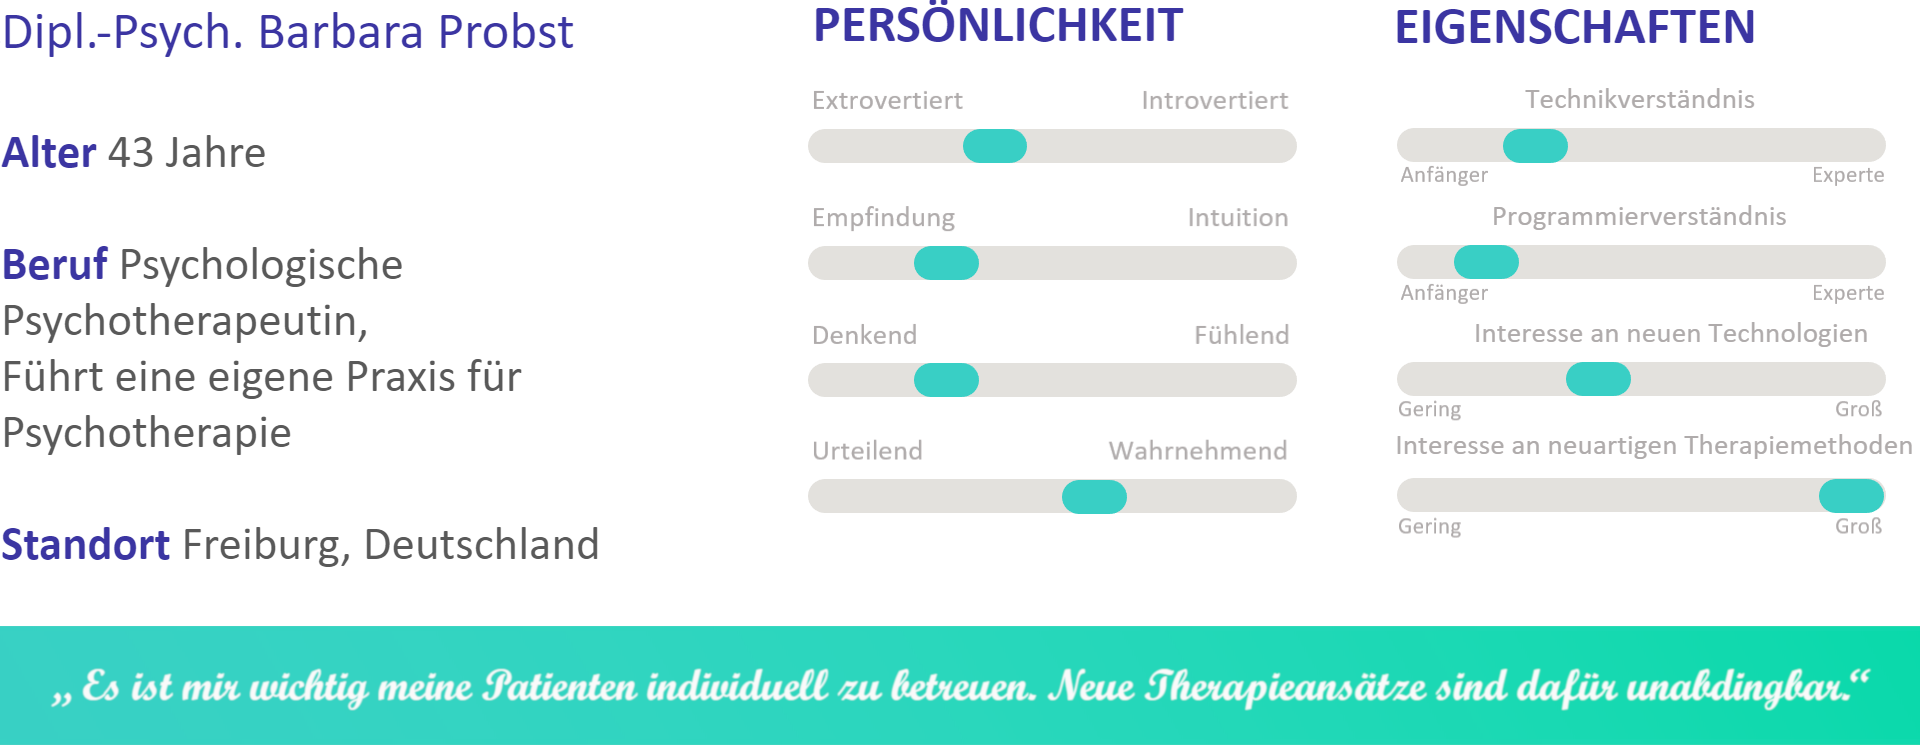
\includegraphics[width=1\textwidth]{pictures/therapeut}
\caption{Eckdaten der fiktiven Therapeutin \emph{Dipl.-Psych. Barbara Probst}}
\label{therapeut}
\end{figure}

\paragraph{Profil}
\emph{Dipl.-Psych. Barbara Probst} ist staatlich geprüfte psychologische Psychotherapeutin. Sie führt eine eigene Praxis. In dieser behandelt sie Patienten mit verschiedenen Störungen mit Krankheitswert. Ihr Spezialgebiet ist die Angststörung.

Sie wendet verschiedene Therapieansätze an. Diese werden individuell auf Persönlichkeit, Krankheitsverlauf und Symptomen des Patienten ausgewählt und zugeschnitten. Dabei nutzt sie altbewährte, wie auch neue Therapieansätze. Ihr Interesse gilt insbesondere neuartigen Therapiemethoden im Bereich der Angststörung. In ihrer Freizeit beschäftigt sie sich deshalb mit Fachjournalen. Sobald sie eine neue vielversprechende und geprüfte Therapiemethode entdeckt, notiert sie sich verschiedene Ansätze um diese auf geeignete Patienten zu übertragen. Dabei sind besonders Ansätze interessant, die neuartige Technologien verwenden.

Da ihr Stundenplan voll belegt ist muss die Übertragung neuer Therapiemethoden leicht und schnell gehen. Falls neue Technologien notwendig sind, sollen diese so leicht zu bedienen sein, dass kein Mehraufwand in Dokumentation und Planung entsteht. Außerdem ist es wichtig, dass eingesetzte Technologien wenig Aufwand und Expertenwissen benötigen um diese entsprechend einzurichten und zu bedienen.

\paragraph{Ziele}
\begin{itemize}
\item Austesten neuer Therapiemethoden
\item Einsatz neuer Technologien in Verbindung mit Psychotherapie
\item Neue Technologien sollten keinen Mehraufwand an Dokumentation darstellen
\item Neue Technologien und Therapien sollten keinen Mehraufwand an Planung darstellen
\item Einsatz neuer Therapiemethoden trotz wenig Zeit
\item Leicht integrierbar in den Alltag und das System eines Psychotherapeuten
\item Geringe Kosten in der Anwendung
\end{itemize}

\subsubsection{Patient}
Der Patient nutzt auf seinem Smartphone die \emph{TherapyBuilder}-App. Diese führt die Therapien aus, die dem Patienten vom Therapeut zugeordnet wurde. Betrachtet werden das Profil und die Ziele der fiktiven Patienten \emph{Jonas Vogt}.

\begin{figure}[h]
\centering
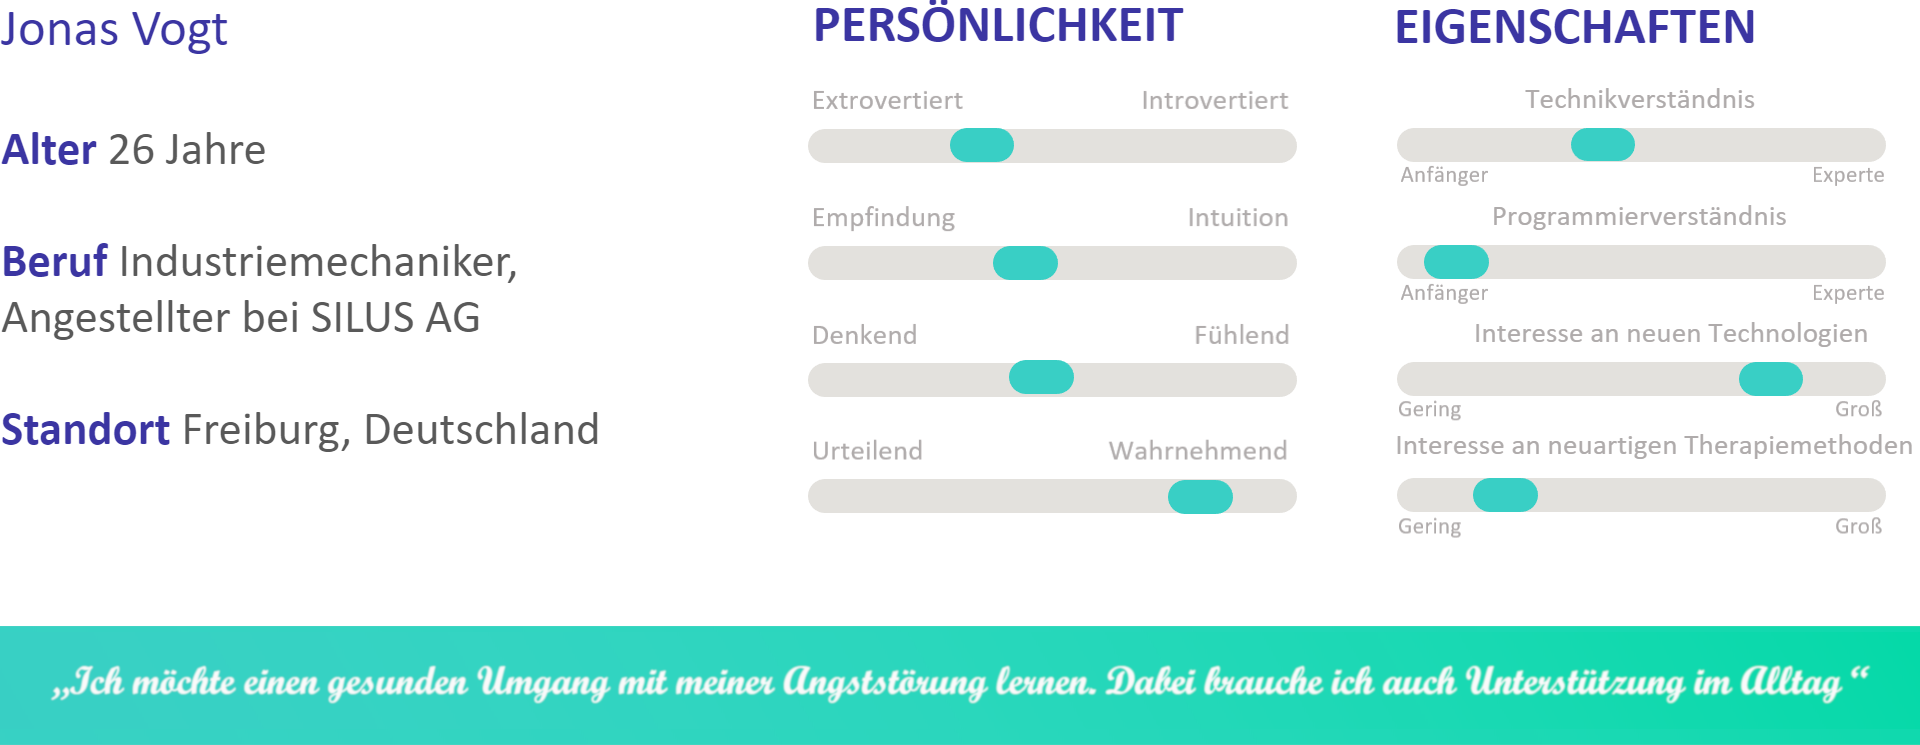
\includegraphics[width=1\textwidth]{pictures/patient}
\caption{Eckdaten des fiktiven Patienten \emph{Jonas Vogt}}
\label{patient}
\end{figure}

\paragraph{Profil}
\emph{Jonas} ist Industriemechaniker aus Freiburg. Er ist seit 3 Jahren Angestellter bei SILUS AG. Nach einem Jahr wurde er zum Schichtleiter befördert. Die Arbeit macht ihm sehr viel Freude. Er ist pflichtbewusst und nimmt seine Verantwortung als Schichtleitung ernst. Er beschäftigt sich in seiner Freizeit fast täglich mit neuen Strategien und Techniken für einen effizienten Schichtbetrieb. Aufgrund seines fachlichen Wissens und Engagements tauschen sich Arbeitskollegen wie Chefs gerne über neue Strategien mit ihm aus.

Neben seinem Beruf interessiert er sich für neue Technik-Gadgets, Spielekonsolen und Multimedia. In seiner Freizeit trifft er sich gerne mit Freunden zum Feiern, gemeinsamen Kochen aber auch zu gemütlichen Film und Spieleabenden. Er verabredet sich häufig über diverse Messenger und teilt über diese gerne Artikel über neue Technik-Gadgets.

\emph{Jonas} hat eine Angststörung die als Begleiterscheinung eines Burn-outs während der Ausbildung auftrat.  Derzeit wartet er auf seine erste Therapiesitzung bei \emph{Dipl.-Psych. Barbara Probst}. Während der Wartezeit nutzt er einen Chatbot. Diesen setzt er ein sobald er sich unwohl fühlt und die Angststörung auftritt. Seine Psychotherapeutin empfahl \emph{Jonas} diesen Chatbot während der Wartezeit zu nutzen.

\paragraph{Ziele}
\begin{itemize}
\item Behandeln der Angststörung
\item Hilfe im Alltag wenn Angststörung auftritt
\item Einfache Anwendung der Hilfe
\item Hilfe jederzeit erreichbar
\item Hilfe leicht in Alltag integrierbar
\end{itemize}


\subsection{Studienbetrachtung}
Für die Anforderungsanalyse werden mehrere Studien betrachtet. Diese liegen der Firma \emph{movisens GmbH} in unterschiedlichen Formaten vor. Ablauf und Inhalte der jeweiligen Studie wurden in PowerPoint-Folien, Excel und Bildern, wie beispielsweise in Abbildung \ref{studie}, beschrieben. Jede Studie besitzt Inhalte, die in Form eines Chats umgesetzt werden könnten. Die Studien beinhalten Therapien, die in dieser evaluiert werden. Die Therapien setzen sich aus verschiedenen Stilmitteln zusammen. So finden sich Dialoge die aus Input und Output-Formaten bestehen. Die Input-Formate repräsentieren Formate, die dem Patienten angeboten werden um Daten einzugeben. Die Output-Formate beinhalten Formate, die dem Patienten angezeigt werden. Die Therapien bestehen aus Übungen, Interventionen und Selbstüberwachung.

\begin{figure}[h]
\centering
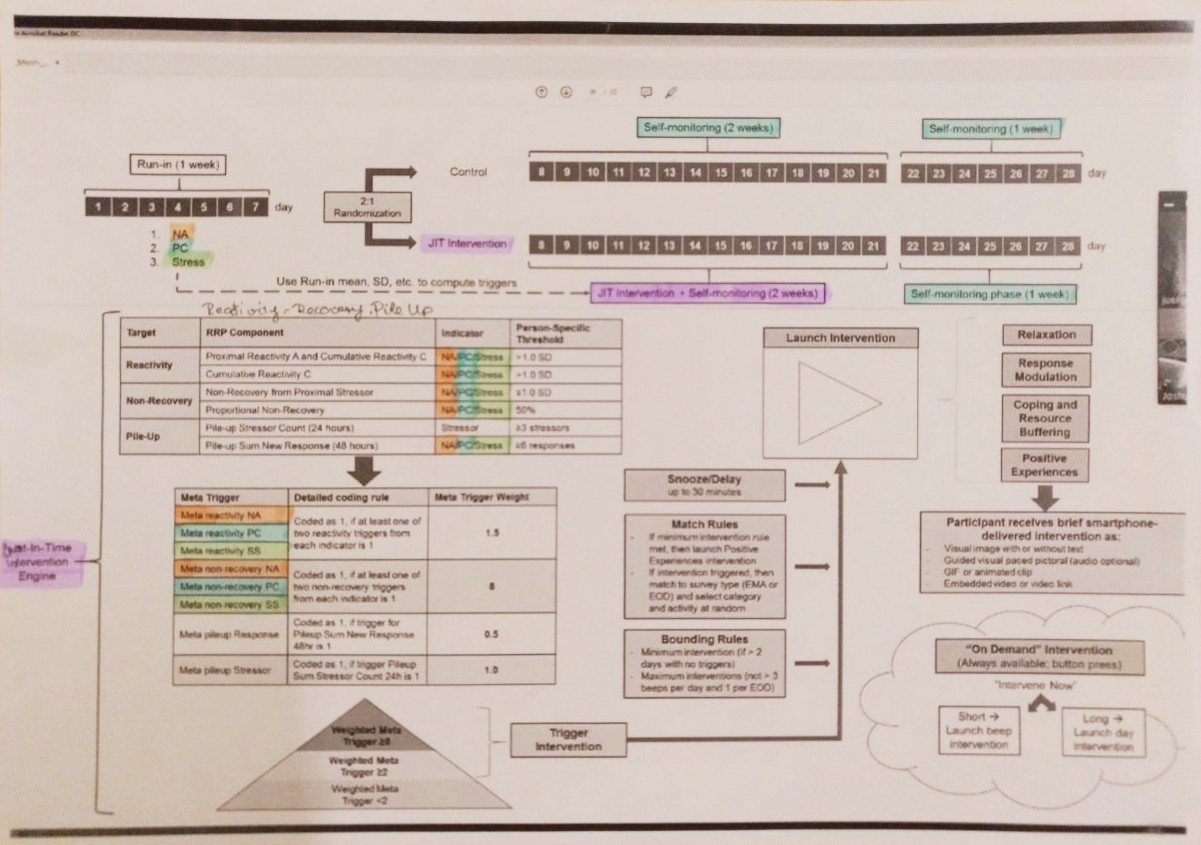
\includegraphics[width=1\textwidth]{pictures/studie}
\caption{Eckdaten des fiktiven Forschers \emph{Prof. Dr. Richard Weimer}}
\label{studie}
\end{figure}

Um eine Therapie umzusetzen, werden als Output-Formate Textausgaben, Video, Audio, und Bilder benötigt. Als Input-Formate für den Patienten werden Texteingabe, ganze Zahlen, rationale Zahlen, Likert-Skalen, visuelle Analogskalen, Einfach- wie Mehrfachauswahl, Zeiteingabe und eine Datumseingabe benötigt. 
 
Da auch Daten erhoben werden, benötigt es Variablen. In diesen werden Antworten und berechnete Werte gespeichert. Die Werte der Variablen können dem Patienten im Text präsentiert werden aber auch den Verlauf der Therapie beeinflussen. So können dem Patienten beispielsweise verschiedene Texte, Übungen oder Interventionen präsentiert werden. Die entsprechenden Inhalte werden zu unterschiedlichen Zeiten und Bedingungen ausgelöst. Auslöser können ein erreichtes Datum, vorgegebene Zeit, Therapeut, Patient oder verschiedene Bedingungen sein. Um diese Übersicht zu erhalten, wurde der zeitliche Ablauf der betrachteten Studien in einem Zeitstrahl abgebildet. Diese zeitliche Skizzierung wird in Abbildung \ref{studien} dargestellt.

\begin{figure}[h]
\centering
\includegraphics[width=1\textwidth]{pictures/studien}
\caption{Die zeitliche Abbildung verschiedener Studien in Form eines Zeitstrahls}
\label{studien}
\end{figure}

\subsection{Defizite der betrachteten Technologien}
In Kapitel \ref{ch:Forschungsstand} werden verschiedene Technologien vorgestellt, die für eine Umsetzung eines \emph{TMA} in Frage kommen. Die dort erläuterten Defizite werden hier in Kurzform zusammengefasst.

\subsubsection{Grafische Programmiersprachen}
Betrachtet wurden Chatbot-Plattformen und allgemeine grafische Programmiersprachen. Chatbot-Plattformen fokussieren sich zumeist auf Marketing, Vertrieb und Support. Die Umsetzung von Studien, die für die Anforderungsanalyse betrachtet wurden, gestaltet sich in diesen Plattformen schwierig. Diese lassen entsprechende Elemente, wie Likert-Skalen, visuelle Analogskalen und eine Patientenverwaltung vermissen. Konversationen als Baum oder Diagramm darzustellen, ist zwar leicht verständlich, allerdings werden diese schnell unübersichtlich wenn mehrere bedingte Pfade eingesetzt werden und die Komplexität der Konversation steigt. Die Gesamtansicht der Konversationen wird demnach auch schwer lesbar. Entweder müssen Verläufe durch scrollen und durchhangeln nachvollzogen werden oder diese werden durch die eingebaute Zoom-Funktion schlechter erkennbar und auffindbar. Manche Plattformen bieten zusätzlich die Möglichkeit, fehlende Funktionen zu implementieren. Die benötigt allerdings Programmiererfahrung. Generell sind bei der Verwendung dieser Plattformen, für eine Umsetzung entsprechender Therapien, mit Einschränkungen oder größeren Einarbeitungszeiten zu rechnen.

Die allgemeinen Programmiersprachen hingegen spezialisieren sich stark auf bestimmte Domänen. Das Baukastenprinzip gewährleistet zwar viel Flexibilität und ist leicht verständlich in der Bedienung, allerdings wird bei steigender Komplexität das entwickelte System leicht unübersichtlich und schwer nachvollziehbar.

\subsubsection{Auszeichnungssprachen}
Die Verwendung von Auszeichnungssprachen bieten visuell zwar eine Trennung aber keine klare Übersicht über den Verlauf einer Konversation. Es benötigt Konzepte um zeitliche Abfolgen einer Therapie, Verzweigungen und Bedingungen zu realisieren und klar darzustellen. Hinzu kommt, dass die Syntax erlernt werden muss. Außerdem benötigt es einen aufwändigen Syntaxcheck um die Fehlersuche in angelegten Chatbot-Konversationen zu erleichtern.   

\subsubsection{Experience Sampling}
Insbesondere das \emph{movisensXS}-System liefert bereits viele Funktionen, die zur Umsetzung der betrachteten Therapien benötigt werden. Allerdings wurde das System für die Fragebogenentwicklung erstellt und müsste entsprechend angepasst werden um dem Chatbot-Format zu entsprechen.  


\subsection{Anforderungen}
Auf Basis der aufgestellten Persona, Betrachtung der Studien und der Defizite der betrachteten Technologien, wurden funktionale sowie nicht-funktionale Anforderungen aufgestellt, die der Therapiemodellierungsansatz erfüllen sollte. Es wurden mehrere Anforderungen in einem Excel-File beschrieben (vgl. \ref{anforderungen}) und entsprechend priorisiert. In diesem Kapitel werden die Anforderungen mit der höchsten Priorität dargestellt. Hierbei handelt es sich um Anforderungen, die den Therapiemodellierungsansatz grundlegend charakterisieren.

\begin{figure}[h]
\centering
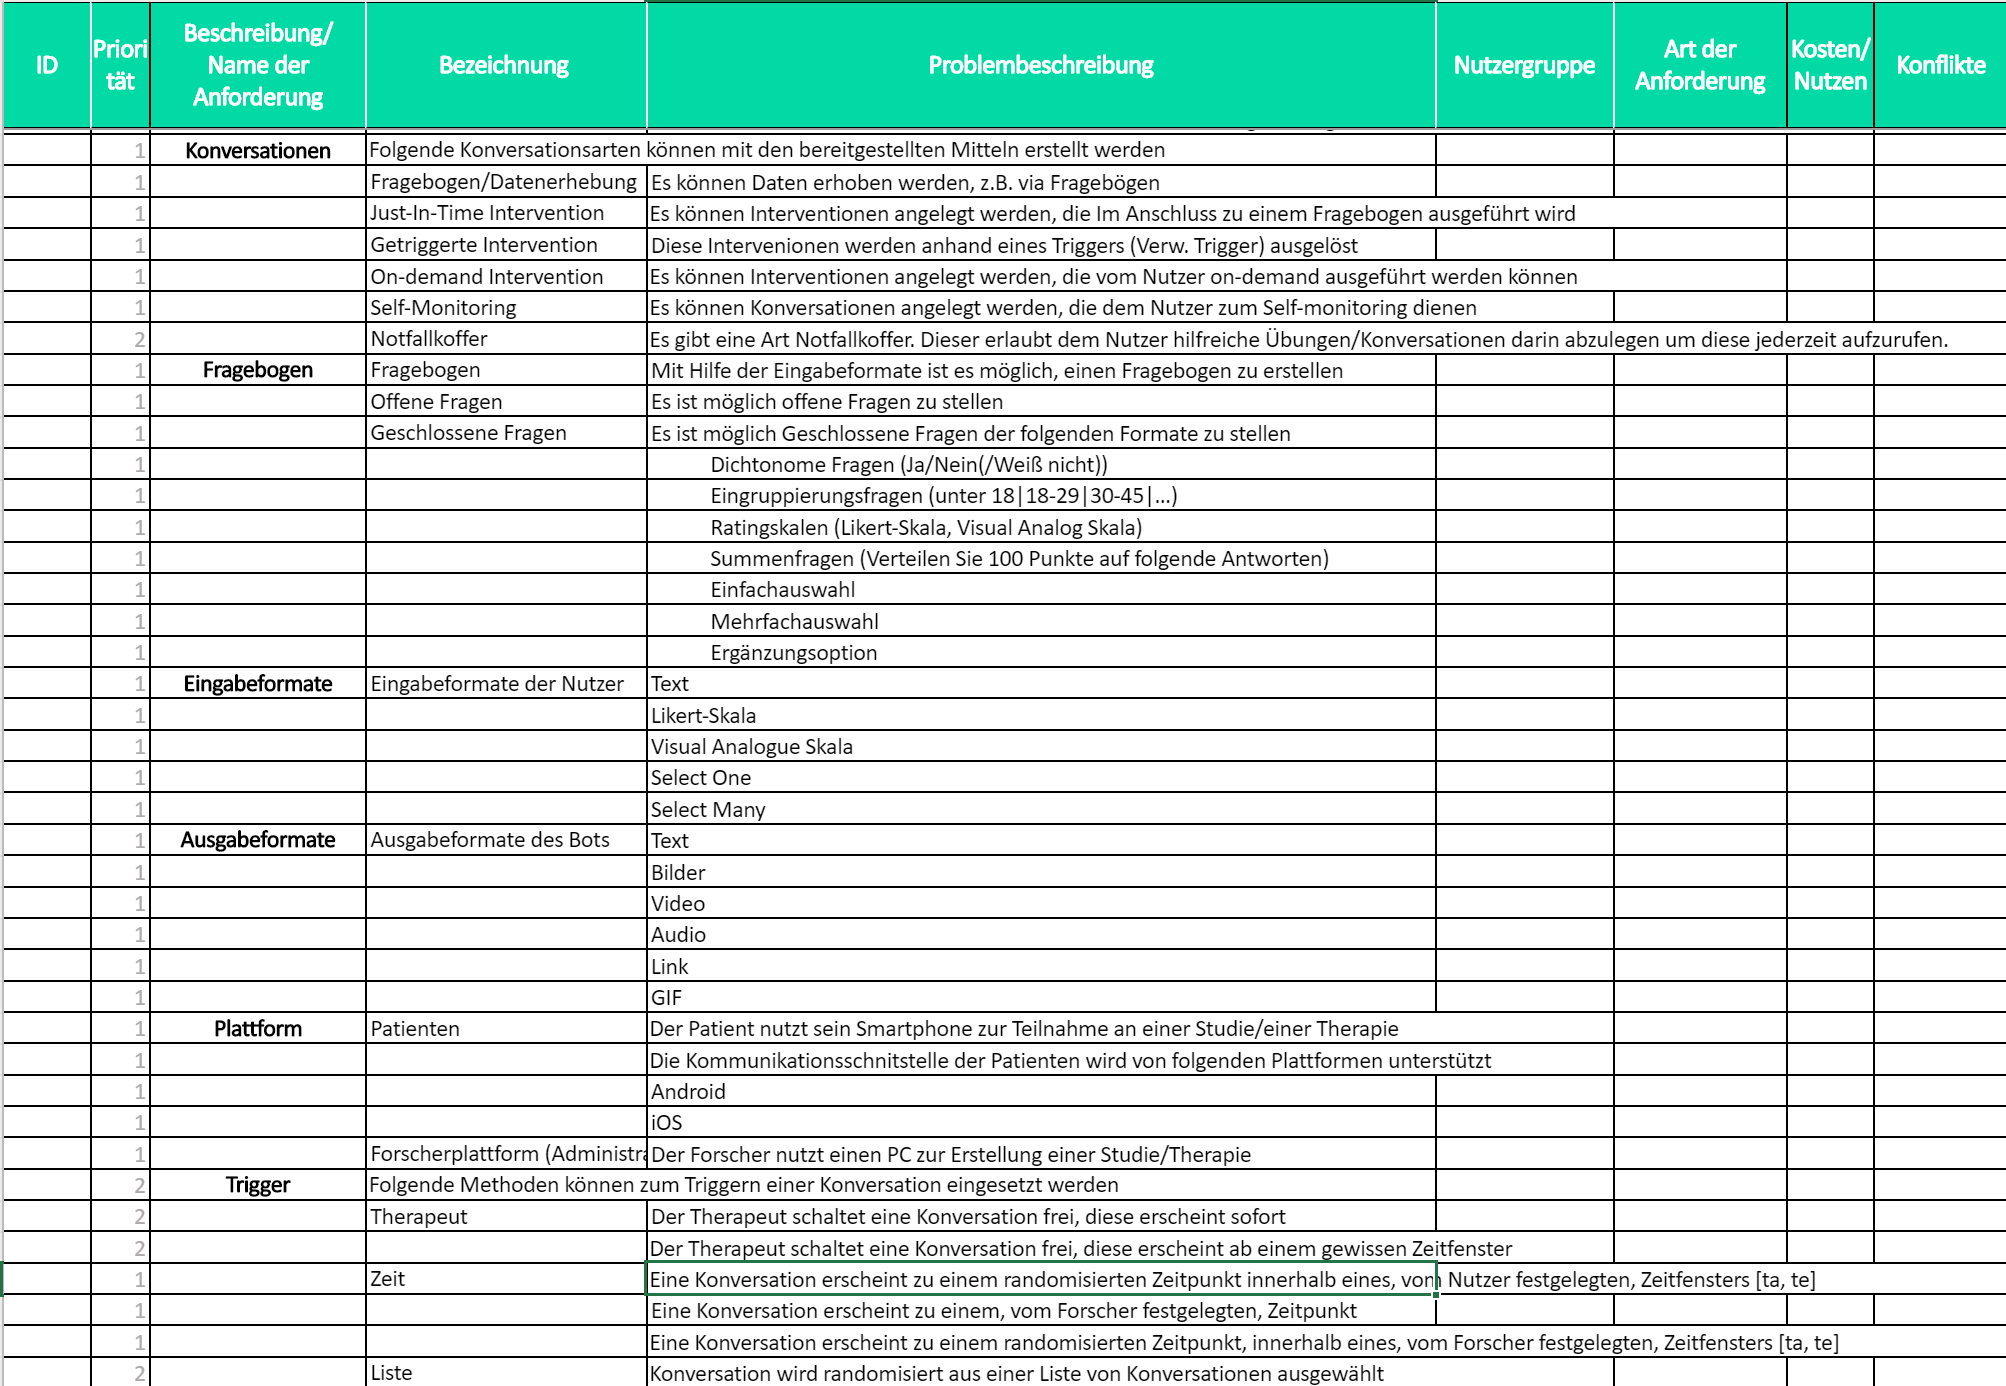
\includegraphics[width=1\textwidth]{pictures/anforderungen}
\caption{Ausschnitt der erstellten Anforderungsliste}
\label{anforderungen}
\end{figure}

\subsubsection{Funktionale Anforderungen}
Im Folgenden werden die Anforderungen beschrieben, die der Zweckbestimmung der Forscher-Plattform dienen.

\paragraph{Konversationen}
Folgende Konversationsarten können mit den bereitgestellten Mitteln erstellt werden.

%\begin{itemize}
%\item Fragebogen/Datenerhebung: Es können Daten erhoben werden, z.B. via Fragebögen
%\item Just-In-Time Intervention: Es können Interventionen angelegt werden, die im Anschluss zu einem Fragebogen ausgeführt werden.
%\item Getriggerte Intervention: Interventionen werden anhand eines Triggers  ausgelöst.
%\item On-demand Intervention: Es können Interventionen angelegt werden, die vom Nutzer on-demand ausgeführt werden können.
%\item Self-Monitoring: Es können Konversationen angelegt werden, die dem Nutzer zum Self-monitoring dienen.
%\end{itemize}
\subparagraph{Fragebogen/Datenerhebung} Es können Daten erhoben werden, z.B. via Fragebögen
\subparagraph{Just-In-Time Intervention} Es können Interventionen angelegt werden, die im Anschluss zu einem Fragebogen ausgeführt werden.
\subparagraph{Getriggerte Intervention} Interventionen werden anhand eines Triggers  ausgelöst.
\subparagraph{On-demand Intervention} Es können Interventionen angelegt werden, die vom Nutzer on-demand ausgeführt werden können.
\subparagraph{Self-Monitoring} Es können Konversationen angelegt werden, die dem Nutzer zum Self-monitoring dienen.

\paragraph{Fragebogen}
Mit Hilfe der Eingabeformate ist es möglich, einen Fragebogen zu erstellen. Mit diesen Mitteln können in den Fragebögen verschiedene Frageformen umgesetzt werden.

%\begin{itemize}
%\item Offene Fragen: Es ist möglich offene Fragen zu stellen.
%\item Geschlossene Fragen: Es ist möglich Geschlossene Fragen der folgenden Formate zu stellen: Dichtonome Fragen (Ja/Nein(/Weiß nicht)), Eingruppierungsfragen (unter 18|18-29|30-45|…), Ratingskalen (Likert-Skala, Visual Analog Skala), Summenfragen (Verteilen Sie 100 Punkte auf folgende Antworten), Einfachauswahl, Mehrfachauswahl, Ergänzungsoption
%%\begin{itemize}
%%\item Dichtonome Fragen (Ja/Nein(/Weiß nicht))
%%\item Eingruppierungsfragen (unter 18|18-29|30-45|…)
%%\item Ratingskalen (Likert-Skala, Visual Analog Skala)
%%\item Summenfragen (Verteilen Sie 100 Punkte auf folgende Antworten)
%%\item Einfachauswahl
%%\item Mehrfachauswahl
%%\item Ergänzungsoption
%%\end{itemize}
%\end{itemize}

\subparagraph{Offene Fragen} Es ist möglich offene Fragen zu stellen.
\subparagraph{Geschlossene Fragen} Es ist möglich Geschlossene Fragen der folgenden Formate zu stellen: Es ist möglich Geschlossene Fragen der folgenden Formate zu stellen: Dichtonome Fragen (Ja/Nein(/Weiß nicht)), Eingruppierungsfragen (unter 18|18-29|30-45|…), Ratingskalen (Likert-Skala, Visual Analog Skala), Summenfragen (Verteilen Sie 100 Punkte auf folgende Antworten), Einfachauswahl, Mehrfachauswahl, Ergänzungsoption


\paragraph{Eingabeformate} Die Eingabeformate der Nutzer	bestehen aus folgenden Elementen
\begin{itemize}
\item Freie Texteingabe
\item Likert-Skala
\item Visual Analogue Skala
\item Select One
\item Select Many
\end{itemize}
%\subparagraph{Freie Texteingabe}
%\subparagraph{Likert-Skala}
%\subparagraph{Visual Analogue Skala}
%\subparagraph{Select One}
%\subparagraph{Select Many}

\paragraph{Ausgabeformate} Die Ausgabeformate des Bots bestehen aus folgenden Elementen
\begin{itemize}
\item Text
\item Bilder
\item Video
\item Audio
\item Link
\item GIF
\end{itemize}
%\subparagraph{Text}
%\subparagraph{Bilder}
%\subparagraph{Video}
%\subparagraph{Audio}
%\subparagraph{Link}
%\subparagraph{GIF}

\paragraph{Trigger}Folgende Methoden können zum Triggern einer Konversation eingesetzt werden
%\begin{itemize}
%\item Therapeut: Der Therapeut schaltet eine Konversation frei, diese erscheint sofort. 
%Der Therapeut schaltet eine Konversation frei, diese erscheint ab einem gewissen Zeitfenster.
%\item Zeit: Eine Konversation erscheint zu einem randomisierten Zeitpunkt innerhalb eines, vom Nutzer festgelegten, Zeitfensters [ta, te], zu einem, vom Forscher festgelegten, Zeitpunkt oder innerhalb eines, vom Forscher festgelegten, Zeitfensters [ta, te]
%\item Liste: Konversation wird randomisiert aus einer Liste von Konversationen ausgewählt
%\item Ausführungsanzahl: Eine Konversation kann anhand einer Anzahl Ausführungen an einem Tag getriggert werden
%\item Nutzer: Ein Nutzer kann selbst eine Konversation starten.
%\item Konversation: Eine Konversation kann durch das Abschließen einer anderen Konversation getriggert werden
%\item Snooze: Eine Konversation wird erneut getriggert nach Zeitpunkt des Snoozes eines Nutzers +t (zB. 30 Minuten)
%\item Variable: Eine Konversation wird durch einen Wert einer Variable getriggert. Dabei gibt es folgende Möglichkeiten: die Variable hat den aktuellen Wert x; die Variable hatte den Wert x zum Zeitpunkt t; die Variable wird ermittelt aus verschiedenen Variablen/Werten durch eine vorgegebene Funktion und erfüllt eine Bedingung.
%\end{itemize}

\subparagraph{Therapeut}Der Therapeut schaltet eine Konversation frei, diese erscheint sofort. 
Der Therapeut schaltet eine Konversation frei, diese erscheint ab einem gewissen Zeitfenster.

\subparagraph{Zeit}Eine Konversation erscheint zu einem randomisierten Zeitpunkt innerhalb eines, vom Nutzer festgelegten, Zeitfensters [ta, te], zu einem, vom Forscher festgelegten, Zeitpunkt oder innerhalb eines, vom Forscher festgelegten, Zeitfensters [ta, te]
\subparagraph{Liste}Konversation wird randomisiert aus einer Liste von Konversationen ausgewählt
\subparagraph{Ausführungsanzahl}Eine Konversation kann anhand einer Anzahl Ausführungen an einem Tag getriggert werden
\subparagraph{Nutzer}Ein Nutzer kann selbst eine Konversation starten 
\subparagraph{Konversation}Eine Konversation kann durch das Abschließen einer anderen Konversation getriggert werden
\subparagraph{Snooze}Eine Konversation wird erneut getriggert nach Zeitpunkt des Snoozes eines Nutzers +t (zB. 30 Minuten)
\subparagraph{Variable}Eine Konversation wird durch einen Wert einer Variable getriggert. Hierbei gibt es folgende Möglichkeiten: die Variable hat den aktuellen Wert x, die Variable hatte den Wert x zum Zeitpunkt t, die Variable wird ermittelt aus verschiedenen Variablen/Werten durch eine vorgegebene Funktion und erfüllt eine Bedingung.

\paragraph{Variablen} Folgende Funktionen und Eigenschaften werden für die Variablen benötigt
\subparagraph{Speichern}Es können Werte unter Variablennamen abgespeichert werden
\subparagraph{Historie}Die Werte, die eine Variable im Verlauf eines Therapiemoduls angenommen hat, werden in einer Historie hinterlegt
\subparagraph{Typen}Eine Variable kann einen der folgenden Typen annehmen
\begin{itemize}
\item String
\item Gleitkommazahl
\item Ganze Zahl 
\item Boolean (Wahr/Falsch)
\item Image 
\item Video
\item Audio
\item Link
\end{itemize}	

\paragraph{Flexible Gestaltung von Triggern}
Da eine Konversation durch verschiedene Bedingungen getriggert werden kann, benötigt es eine flexible Gestaltung der Trigger einer Konversation. Die Anzahl der Trigger soll hierbei flexibel sein. Außerdem sollen verschiedene Bedingungen eingebaut werden können.

\paragraph{Verzweigungen in Konversationen}
Konversationen können Entscheidungen beinhalten, die einen Einfluss auf den weiteren Konversationsverlauf haben. Es ist möglich, Verzweigungen in Konversationen einzubauen und den Fluss, anhand verschiedener Bedingungen, zu steuern. 

\paragraph{Abhängigkeiten zwischen Konversationen}
Konversationen können von anderen Konversationen abhängig sein. Die Abhängigkeiten sind dabei wie folgt:
\begin{itemize}
\item Konversation b kann nur gestartet werden, wenn Konversation a noch nie durchgeführt wurde (b wenn a < 1)
\item Konversation b kann erst gestartet werden, wenn Konversation a genau einmal ausgeführt wurde (b wenn a = 1)
\item Konversation b kann erst gestartet werden, wenn Konversation a mindestens einmal ausgeführt wurde (b wenn a >= 1)  
\end{itemize} 

\subsubsection{Nicht-Funktionale Anforderungen}
Im Folgenden werden die Anforderungen beschrieben, die der Qualität der Forscher-Plattform dienen.

\subparagraph{Anmeldeseite} Nachdem der Nutzer den Link zur TherapyBuilder Forscher-\paragraph{Plattform} in einer Browser Adressleiste eingegeben hat, öffnet sich die Anmeldeseite.

\subparagraph{Startseite}Nach erfolgreicher Anmeldung des Nutzers, wird dieser auf die Startseite weitergeleitet
\subparagraph{Startseite-Inhalt}Die Startseite beinhaltet
\begin{itemize}
\item Logout: Es gibt ein Link zum Ausloggen
\item Account-Einstellungen: Es gibt ein Link zum Aufrufen der Account-Einstellungen
\item Übersicht bereits angelegter Therapie-Module: Es gibt eine Übersicht über alle bereits angelegte Therapie-Module
\item Therapie-Modul hinzufügen: Es gibt eine Schaltfläche zum Hinzufügen eines Therapie-Moduls
\item Therapie-Modul umbenennen: Es gibt eine Schaltfläche zum Umbenennen eines Therapie-Moduls
\item Therapie-Modul entfernen: Es gibt eine Schaltfläche zum Entfernen eines Therapie-Moduls
\item  Therapie-Modul kopieren: Es gibt eine Schaltfläche zum Kopieren eines Therapie-Moduls
\item Therapie-Modul Status: Jedes bereits angelegte Therapie-Modul erhält einen Status. Dieser Status wird auf der Übersichtsseite für jedes Therapie-Modul angezeigt.
\end{itemize}
	
\subparagraph{Bearbeiten} Therapiemodul bearbeiten	Durch Klick auf ein Therapie-Modul, gelangt man auf dessen Bearbeitungsseite
		
\subparagraph{Hinzufügen}Durch Klick auf die "Hinzufügen" Schaltfläche wird ein neues Therapie-Modul angelegt.

\subparagraph{Umbenennen} Durch Klick auf die "Umbenennen" Schaltfläche kann der Nutzer das Modul umbennenen.

\subparagraph{Kopieren} Durch Klick auf die "Kopieren" Schaltfläche kann der Nutzer das Modul kopieren.

\subparagraph{Entfernen} Durch Klick auf die "Entfernen" Schaltfläche öffnet sich ein Dialog zur Eingabe des Wortes "DELETE" um das Entfernen des Therapie-Moduls zu bestätigen.


\section{Ausarbeitung verschiedener Konzepte}
In diesem Kapitel werden verschiedene Konzepte vorgestellt, die später Prototypisch umgesetzt und evaluiert werden. Für ein besseres Verständnis der Konzepte werden vorerst verschiedene Begriffe definiert. Anschließend werden, auf Basis der Begriffsdefinitionen und der Anforderungsanalyse, verschiedene Konzepte vorgestellt. 

\subsection{Begriffsdefinitionen}

Im Rahmen der Konzeption werden verschiedene Begriffe eingeführt, die Klarheit über Struktur und Aufbau einer Therapie geben werden. Unterschieden wird zwischen den Begriffen \emph{Therapie}, \emph{Therapiemodul}, \emph{Chatbot-Konversation}, \emph{Chatbot-Nachricht}, \emph{Werkzeugkasten}. Für ein besseres Verständnis der Zusammenhänge werden Mengendefinitionen abgebildet. Für diese werden die Kürzel aus Abbildung \ref{begriffe} verwendet.


\begin{figure}[h]
	\centering
	\includegraphics[width=.75\textwidth]{pictures/begriffe}
	\caption{Die verwendeten Begriffe und ihre Synonyme.}
	\label{begriffe}
\end{figure}

Insgesamt bestehen zwischen den Begrifflichkeiten Beziehungen die den Aufbau einer Therapie beschreiben. Abbildung \ref{mengeninsg} verdeutlicht den gesamten Aufbau einer Therapie und die Zusammenhänge zwischen einzelnen Elementen. Eine Therapie besteht aus verschiedenen Therapie-Modulen. Diese bilden sich wiederum aus Chatbot-Konversationen. Chatbot-Konversationen können sich aus einfachen Nachrichten zusammenbauen. Es gibt auch Elemente, die in einem Werkzeugkasten als Konversation auftauchen können. Diese können wiederum ein Teil einer Konversation sein und setzen sich ebenfalls aus einfachen Nachrichten zusammen. Die Nachrichten entweder aus Chatbot-Nachrichten oder Patienten-Nachrichten. Die genauen Begrifflichkeiten werden in diesem Kapitel definiert, erklärt und mit Beispielszenarien anhand der entwickelten Persona beschrieben.

\begin{figure}[h]
	\centering
	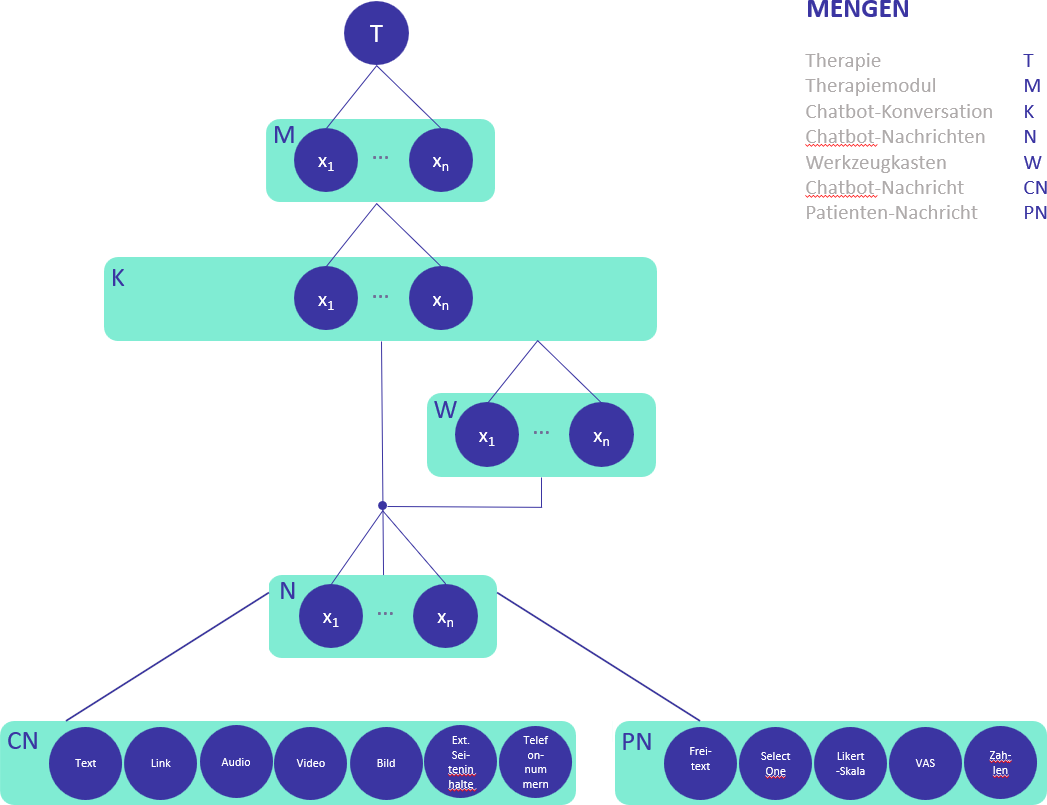
\includegraphics[width=.75\textwidth]{pictures/mengeninsg}
	\caption{Übersicht der Beziehungen aller beschriebenen Mengen}
	\label{mengeninsg}
\end{figure}

\subsubsection{Therapie}
Im Rahmen dieser Arbeit wird unter \emph{Therapie} das Anwenden  einer oder mehrerer Methoden zur Behandlung einer oder mehrerer Störungen mit Krankheitswert oder auch die Aufarbeitung und Überwindung sozialer Konflikte verstanden. Bei diesen Methoden handelt es sich um wissenschaftlich anerkannte psychotherapeutische Verfahren. Den zu behandelnden Störungen mit Krankheitswert wird vorausgesetzt, dass diese als Psychotherapie indiziert sind.

Eine Therapie wird auf genau  einen Patienten zugeordnet. Diese setzt sich aus mehreren Therapiemodulen zusammen. Für die Zusammensetzung der Therapie eines Patienten ist der Psychologische oder Ärztliche Psychotherapeut zuständig.

\paragraph{Definition}
\begin{quote}
Verfahren, Methode zur Heilung einer Krankheit; Heilbehandlung. \cite{PsychThG4:online}
\end{quote}

\begin{quote}
	Eine gezielte, erfolgreiche, medikamentöse Therapie. \cite{44:online}
\end{quote}

\paragraph{Beispiel anhand der aufgestellten Persona}
\emph{Jonas Vogt} ist 26 Jahre und leidet unter den Spätfolgen eines Burnouts. Im Erstgespräch mit seiner Psychologischen Psychotherapeutin \emph{Dipl.-Psych. Barbara Probst} legt diese, basierend auf seinen Erzählungen, eine Therapie fest. Die Therapie besteht aus  mehreren Therapiemodulen. Diese richten sich auf verschiedene Symptome aus. So sieht die Therapie vor \emph{Jonas} zunächst den Umgang mit Panikattacken, Stressbewältigung beizubringen und sein Selbstwertgefühl zu stärken. Dies geschieht durch eine Kombination aus Verhaltens- und tiefenpsychologisch fundierten Therapie.

\begin{figure}[h]
\centering
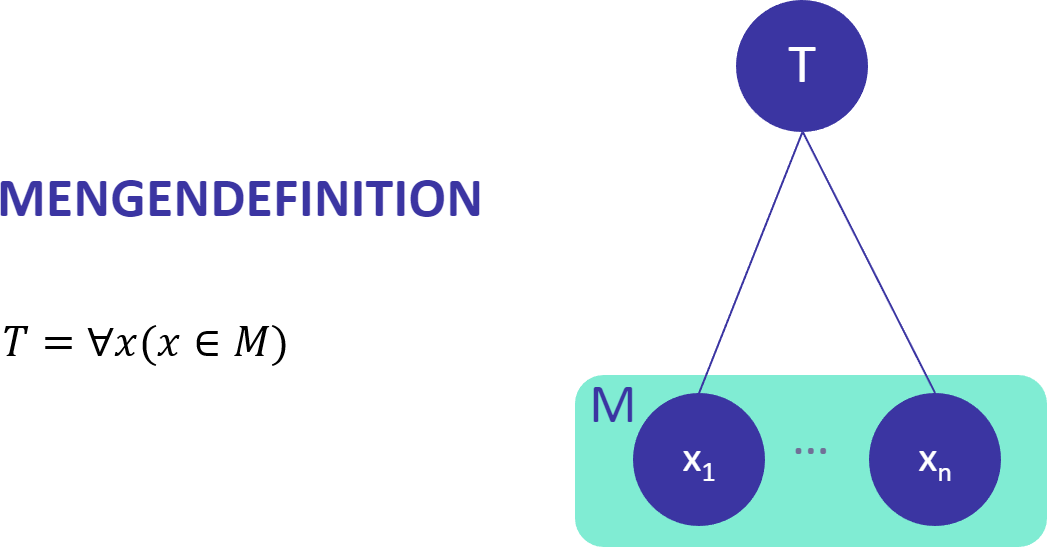
\includegraphics[width=0.5\textwidth]{pictures/therapiedef}
\caption{Aufbau und Beziehungen einer \emph{Therapie}}
\label{therapiedef}
\end{figure}


\subsubsection{Therapiemodul}
Im Rahmen dieses Projekts wird unter \emph{Therapiemodul} das Anwenden  einer Methode zur Behandlung einer Störung mit Krankheitswert oder auch die Aufarbeitung und Überwindung sozialer Konflikte verstanden. Bei diesen Methoden handelt es sich um wissenschaftlich anerkannte psychotherapeutische Verfahren. Den zu behandelnden Störungen mit Krankheitswert wird vorausgesetzt, dass diese als Psychotherapie indiziert sind.

Ein Therapiemodul ist Teil einer Therapie. Das Therapiemodul behandelt ein Aspekt der Therapie.

\paragraph{Definition}
\begin{quote}
Austauschbares, komplexes Element innerhalb eines Gesamtsystems, eines Gerätes o. Ä., das eine geschlossene [Funktions]einheit bildet. \cite{DudenMod70:online}
\end{quote}

\paragraph{Beispiel anhand der aufgestellten Persona}
 \emph{Jonas Vogt} ist 26 Jahre und leidet unter den Spätfolgen eines Burnouts. Seine Psychologische Psychotherapeutin \emph{Dipl.-Psych. Barbara Probst} wendet im Erstgespräch ein Therapiemodul an, welches \emph{Jonas} dabei helfen soll, negative Gedanken zu erkennen und diese für den weiteren Therapieverlauf zu dokumentieren. Ziel des Therapiemoduls ist es, \emph{Jonas} beizubringen, negative Gedanken aufzuschlüsseln und in positive Gedanken umzuformulieren. Im weiteren Verlauf der Therapie wendet \emph{Dipl.-Psych. Barbara Probst} weitere Therapiemodule an um verschiedene Probleme, die zum einen zum Burnout führten und zum anderen aus dem Burnout resultieren, aufzuschlüsseln und \emph{Jonas} den Umgang damit zu erleichtern.

\begin{figure}[h]
\centering
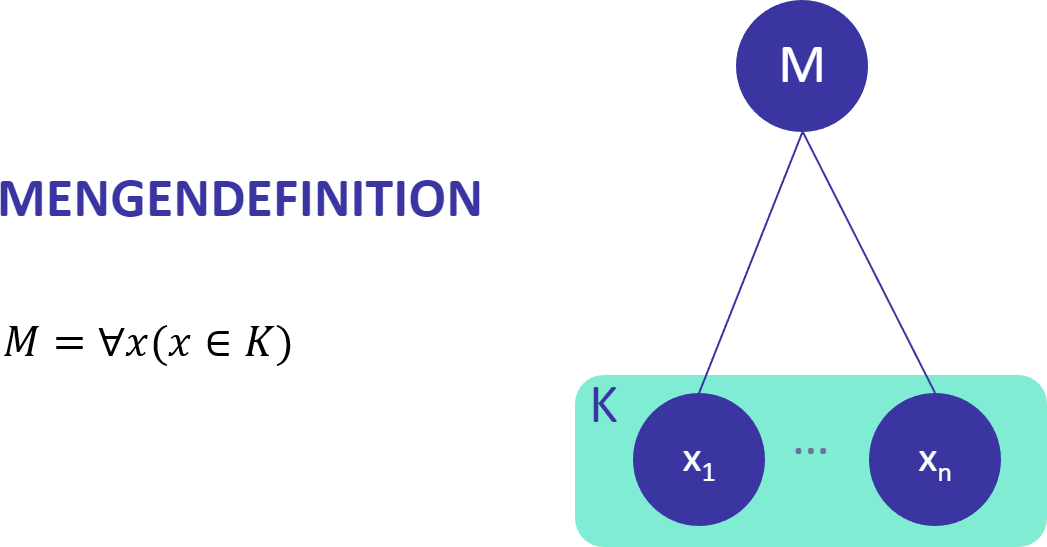
\includegraphics[width=0.5\textwidth]{pictures/moduldef}
\caption{Aufbau und Beziehungen des \emph{Therapiemoduls}}
\label{moduldef}
\end{figure}

\subsubsection{Chatbot-Konversation}
Im Rahmen dieses Projekts wird unter Chatbot-Konversation das Führen  eines Gesprächs mit dem Ziel zur Behandlung/Begleitung einer Störung mit Krankheitswert oder auch die Aufarbeitung und Überwindung sozialer Konflikte verstanden. Die Konversation ist Teil eines Therapiemoduls und kann von Bildern, Video-/Audiomaterial sowie Übungen begleitet werden. Im Kontext des TherapyBuilders wird die Konversation zwischen zwei Parteien geführt: dem Therapeuten oder dem Chatbot und dem Patienten.

\paragraph{Definition}
\begin{quote}
Häufig konventionelles, oberflächliches und unverbindliches Geplauder; Gespräch, das in Gesellschaft nur um der Unterhaltung willen geführt wird. \cite{DudenKon2:online}
\end{quote}

\paragraph{Beispiel anhand der aufgestellten Persona}
\emph{Dipl.-Psych. Barbara Probst} führt pro Therapiesitzung ein Gespräch/eine Konversation mit ihrem Patienten \emph{Jonas Vogt}. In dieser Konversation ermittelt sie \emph{Jonas} aktuellen Zustand, Dinge die in derzeit bewegen und beschäftigen und erklärt ihm den Ursprung seiner Gefühle. Außerdem führt sie mit \emph{Jonas} Übungen durch, die ihm im Alltag helfen können bestimmte wiederkehrende Probleme zu meistern und sein Selbstwert zu stärken.

\begin{figure}[h]
\centering
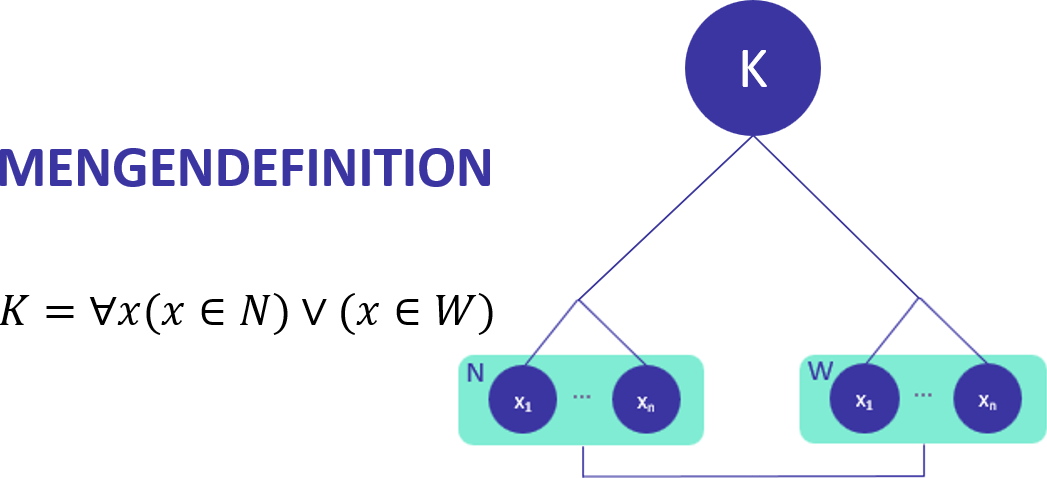
\includegraphics[width=0.5\textwidth]{pictures/konvesationdef}
\caption{Beziehungen der Chatbot-Konversation}
\label{therapiedef}
\end{figure}


\subsubsection{Chatbot-Nachricht}
Im Rahmen dieses Projekts wird unter Chatbot-Nachricht ein Teil einer Therapie-Konversation verstanden. Im Kontext des TherapyBuilders wird zwischen Chatbot und Patient eine Konversation, bestehend aus Nachrichten, aufgebaut. Unterschieden wird innerhalb dieser Konversation zwischen Nachrichten des Patienten und Nachrichten des Chatbots unterschieden. Die Nachrichten des Chatbots können aus folgenden Elementen bestehen: Text, Link, Audio, Video, Bild, Externe Seiteninhalte (Statistiken - Iframe), Telefonnummern. Die Nachrichten des Nutzers können aus folgenden Elementen bestehen: Select One (Quick Reply), Freitext, Likert-Skala, Zahlen (GK, FKZ, Datum, Zeit), Visual-Analog-Skala (VAS).

\paragraph{Definition}
\begin{quote}
Mitteilung, die jemandem in Bezug auf jemanden oder etwas [für ihn persönlich] Wichtiges die Kenntnis des neuesten Sachverhalts vermittelt. \cite{DudenNac9:online}
\end{quote}

\paragraph{Beispiel anhand der aufgestellten Persona}
\emph{Jonas Vogt} erhielt im Erstgespräch mit seiner Psychologischen Psychotherapeutin \emph{Dipl.-Psych. Barbara Probst} die Empfehlung die Anwendung „TherapyBuilder“ auf dessen Smartphone zu installieren. \emph{Jonas} soll diesen zunächst bis zum ersten Behandlungstermin nutzen. Frau \emph{Dipl.-Psych. Barbara Probst} legt für \emph{Jonas} fest, welche Therapiemodule bis dahin für \emph{Jonas} zur Verfügung stehen. \emph{Jonas} kommuniziert täglich mit dem Chatbot des TherapyBuilders. Die Art der Nachrichten des Chatbots sowie des Anwenders \emph{Jonas} wurden bereits als Therapiemodul konfiguriert und festgelegt. Der Chatbot kommuniziert mit \emph{Jonas} via Text, Link, Audio, Video, Bild, Externe Seiteninhalte (Statistiken - Iframe), Telefonnummern. \emph{Jonas} selbst nutzt Eingabeformate wie Select One (Quick Reply), Freitext, Likert-Skala, Zahlen (GK, FKZ, Datum, Zeit), Visual-Analog-Skala (VAS). Wann er welche als Nachricht an den Chatbot versendet, ist innerhalb des Therapiemoduls geregelt.

\begin{figure}[h]
\centering
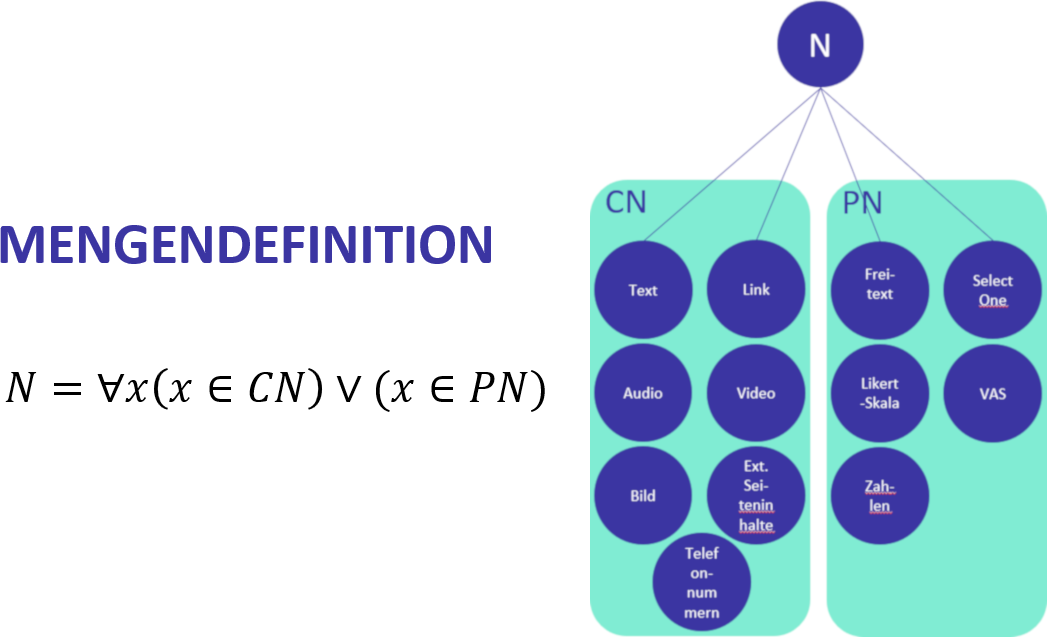
\includegraphics[width=0.5\textwidth]{pictures/nachrichtdef}
\caption{Beziehungen der Chatbot-Nachrichten}
\label{therapiedef}
\end{figure}

\subsubsection{Werkzeugkasten}
Im Rahmen dieses Projekts wird unter Werkzeugkasten ein Teil eines Therapie-Moduls verstanden welches Techniken (=Werkzeuge) sammelt, die jederzeit wiederholt ausgeführt werden können. Diese sollen den Nutzer unterstützen bestimmte (Denk- oder Verhaltens-) Muster zu erkennen und diese aufzulösen. Dies geschieht unter Zuhilfenahme bestimmter Techniken. In diesem Teil wird der Nutzer angeleitet eine bestimmte Vorgehensweise durchzuführen, um diese Techniken auf bestimmte Denk- oder Verhaltensmuster anzuwenden. Der Nutzer kann diese Techniken jederzeit im Werkzeugkasten als Werkzeug aufrufen wenn benötigt.

\paragraph{Definition}
\begin{quote}
Kasten zur Aufbewahrung von Werkzeug. \cite{DudenWer23:online}
\end{quote}

\paragraph{Beispiel anhand der aufgestellten Persona}
\emph{Dipl.-Psych. Barbara Probst} rät \emph{Jonas Vogt} bis zum ersten Behandlungstermin die Therapiemodule durchzuführen, die sie in \emph{Jonas} Therapieplan ablegt. Sie unterrichtet \emph{Jonas}, dass diese Hilfreiche Werkzeuge für bestimmte Denk- und Verhaltensmuster enthalten. Diese müssen durch einen Fortschritt im Therapiemodul freigeschaltet und können ab diesem Zeitpunkt jederzeit von \emph{Jonas} aufgerufen werden. Das erste Werkzeug welches \emph{Jonas} aktiviert, ist das Werkzeug für das Auflösen negativer Gedanken. Sobald \emph{Jonas} negative Gedanken hat, führt er dieses Werkzeug erneut aus um die negativen Gedanken aufzulösen.

\begin{figure}[h]
\centering
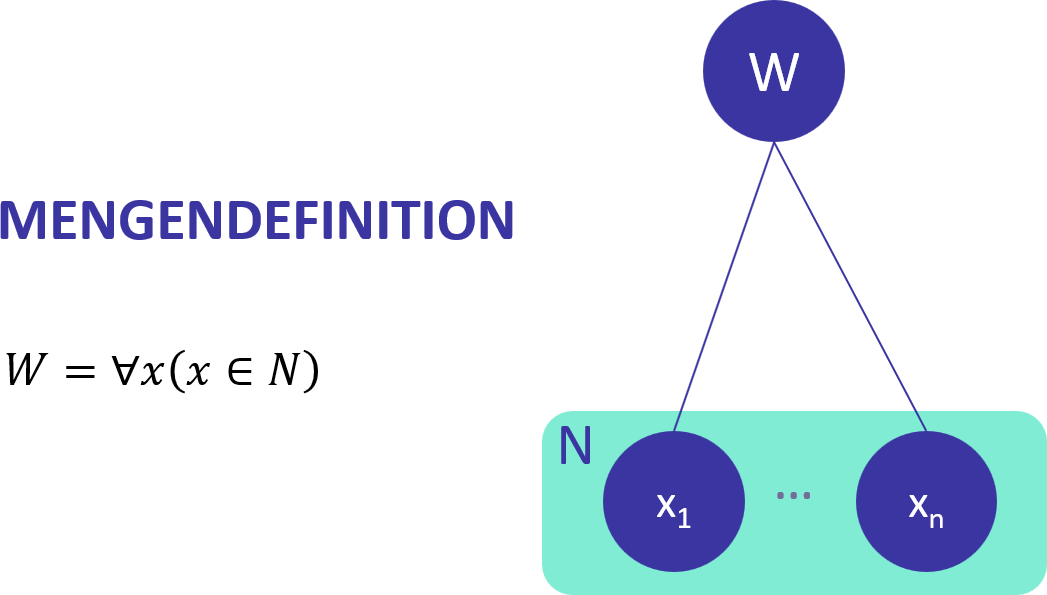
\includegraphics[width=0.5\textwidth]{pictures/toolboxdef}
\caption{Beziehungen der Mengen}
\label{therapiedef}
\end{figure}



\subsection{Konzepte}
Im Verlauf der Konzept-Entwicklung wurden verschiedene Ansätze für die Anforderungen betrachtet. Eine der Überlegungen war, eine angepasste Auszeichnungssprache zu entwickeln, die es Forschern ermöglicht, Therapie-Module niederzuschreiben. Durch verschiedene Befehle sollten Chatbot-Nachrichten, Patienten-Nachrichten sowie verschiedene Bedingungen für den Konversationsfluss, beschrieben werden und sich zu einer Konversation zusammenfügen. Gleichzeitig sollte daraus eine Echtzeitvorschau des Konversationsflusses entstehen. Betrachtet man allerdings die Persona Beschreibung des Forschers, so fällt dieser Ansatz raus. Eine Auszeichnungssprache benötigt Einarbeitungszeit und leichte, wenn auch nicht viele, Programmierkenntnisse. Für Forscher mit wenig Technikverständnis könnte dies eine Hürde bilden das Programm zu nutzen. 

Nach einer weiteren Betrachtung der Anforderungen wurde entschieden, eine grafische Programmiersprache zu entwickeln. Diese bietet die Vorteile, dass keine tiefgreifenden Programmierkenntnisse benötigt werden um eine Therapie zu modellieren. Eine erste Überlegung ist, die grafische Programmiersprache nach der Begriffsdefinition dieses Kapitels aufzubauen. Eine Therapie setzt sich aus verschiedenen Therapiemodulen zusammen. Ein Therapiemodul beinhaltet das Skript, welches verschiedene Storylines und die zeitlichen Abfolgen beschreibt. Nach dieser Betrachtung wurde ein Konzept ausgearbeitet, welches die Konfiguration der zeitlichen Abfolge ermöglicht. Die Skizzierung des Konzepts kann in Abbildung \ref{storylinekonz} betrachtet werden.

\begin{figure}[h]
\centering
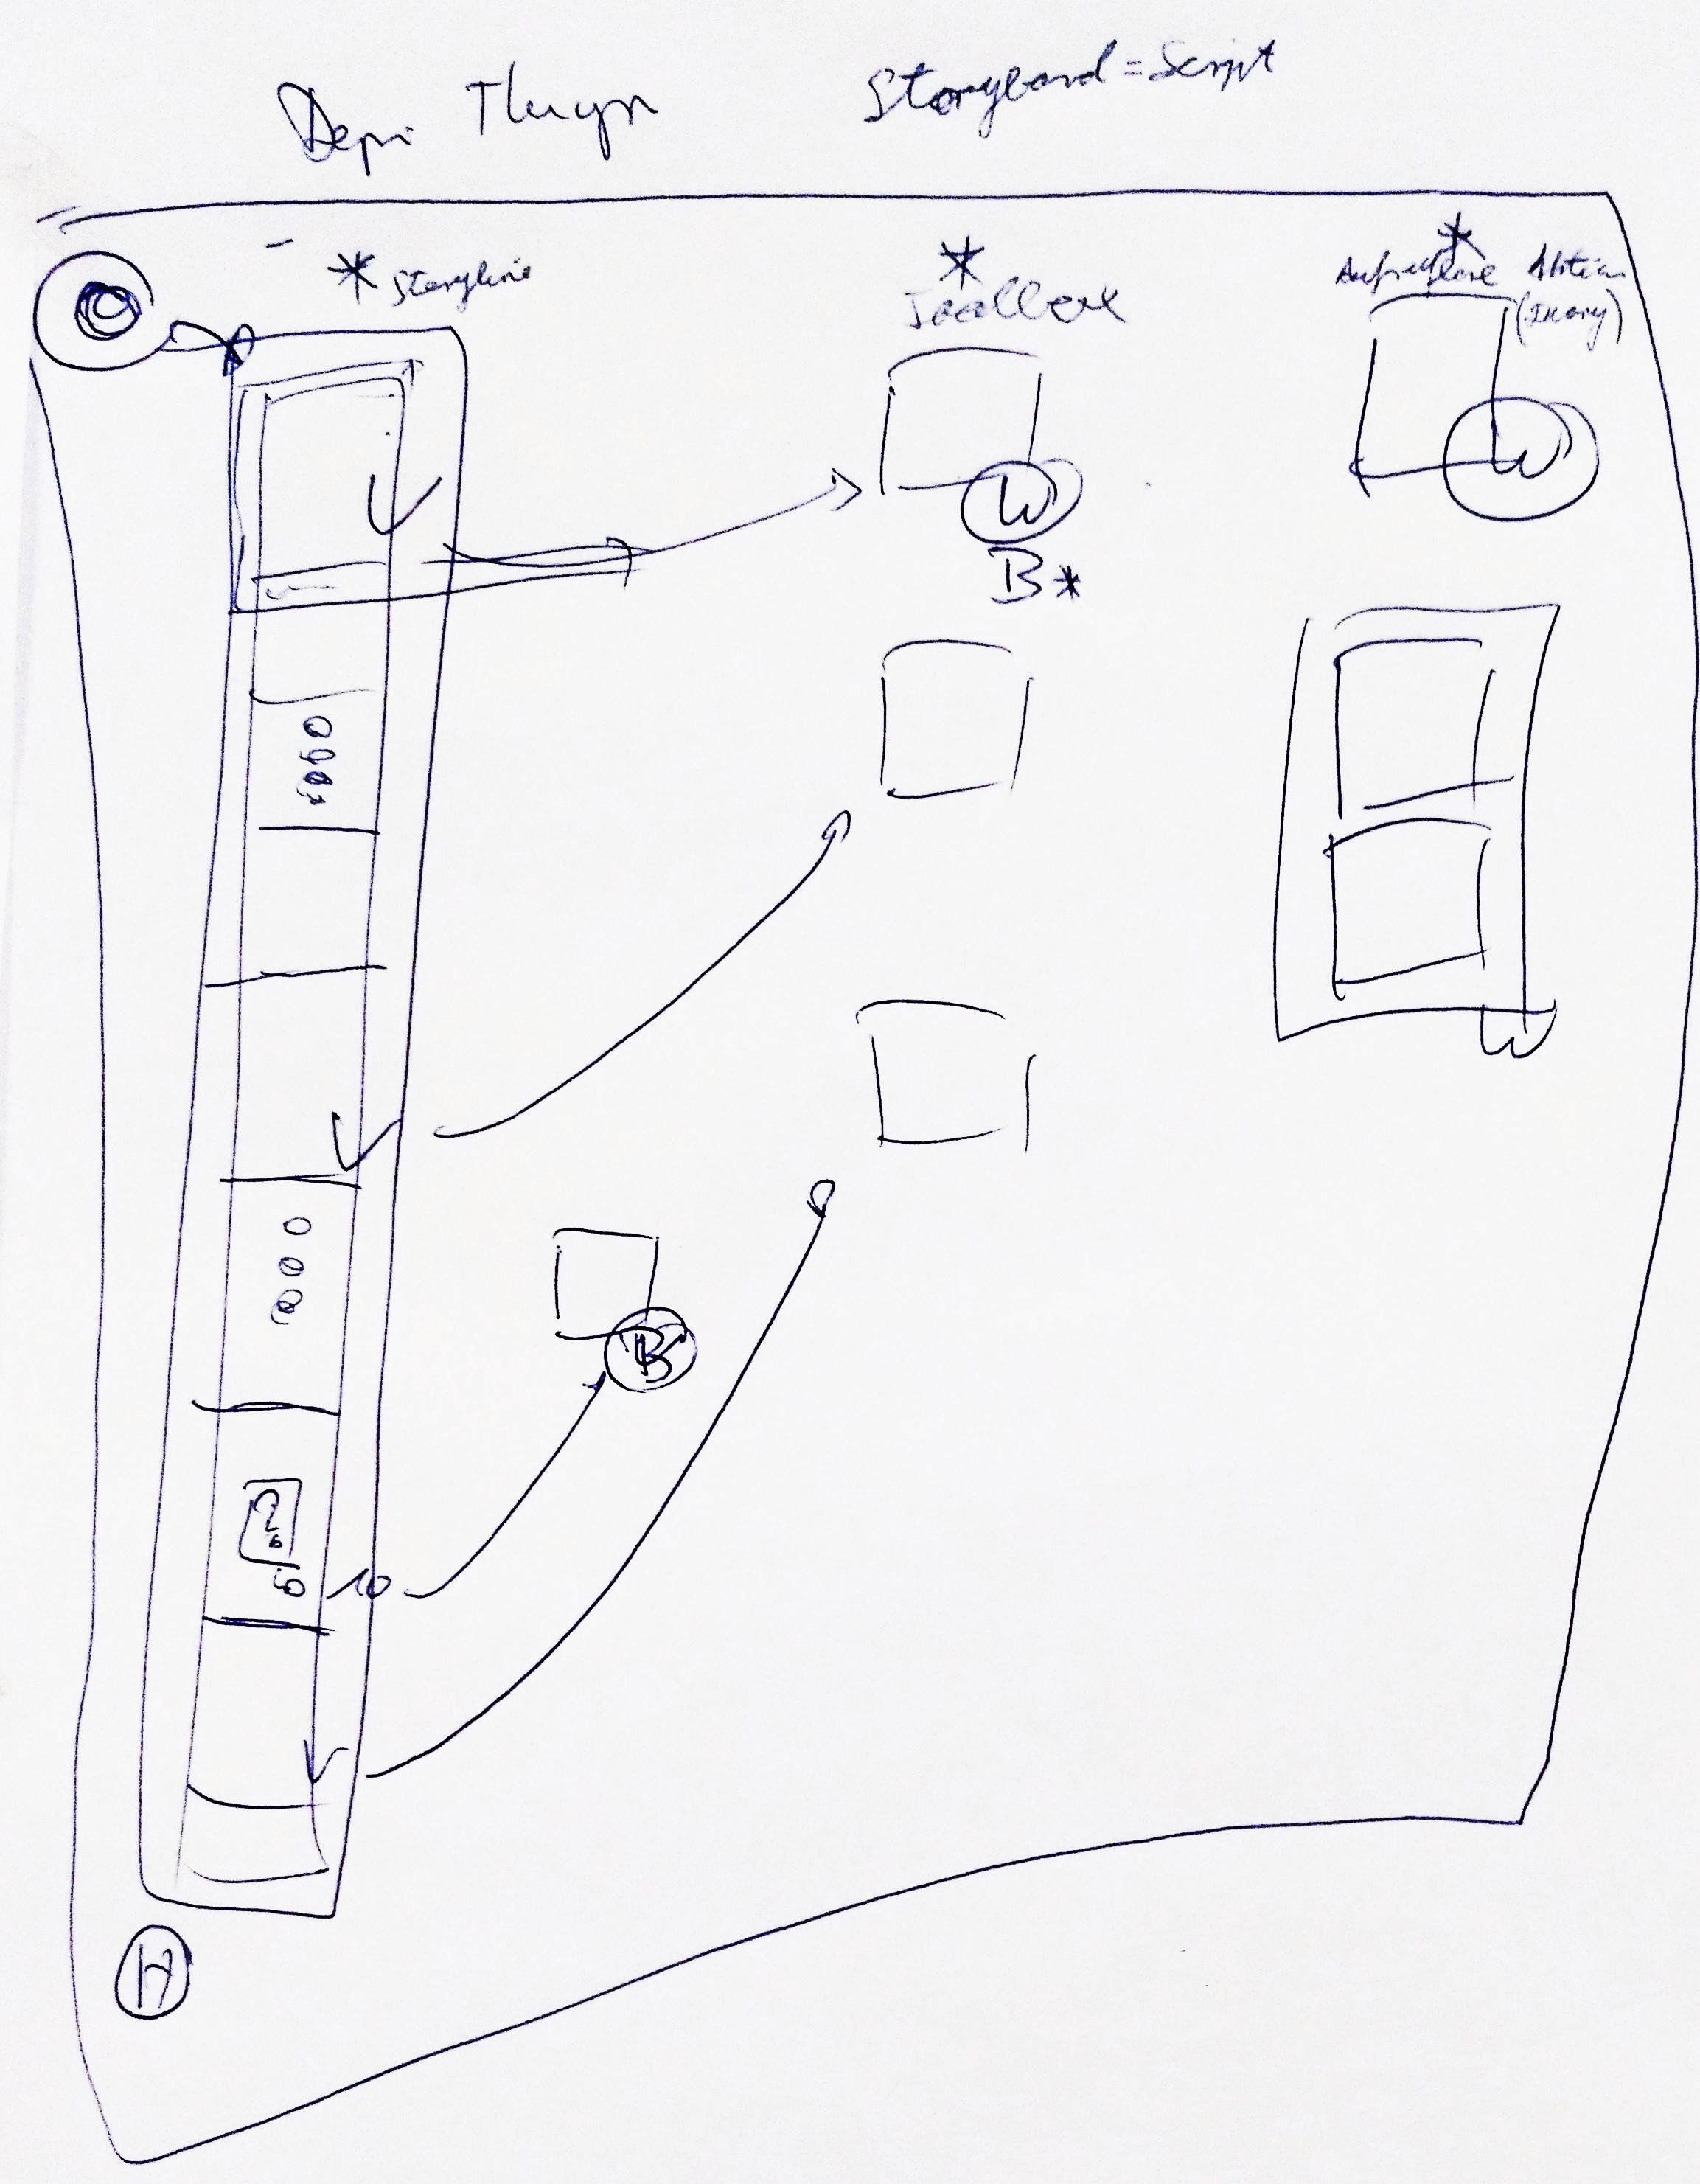
\includegraphics[width=0.5\textwidth]{pictures/storylinekonz}
\caption{Skizze des Konzepts, welches nach den Begriffsdefinitionen ausgearbeitet wurde. }
\label{storylinekonz}
\end{figure}

Die Überlegung des Konzepts ist, die Chatbot-Konversation als Storyline zu verbildlichen. Ein Therapiemodul darf dabei als Drehbuch angesehen werden. In einer Übersicht wird ein Strang dargestellt. Dieser Strang repräsentiert das Skript. Dem Skript können aufeinander folgend Storylines angehängt werden. Einzelne Storylines können als Toolbox-Items definiert werden. Toolbox-Items haben die Möglichkeit jederzeit vom Patienten aufgerufen zu werden. Jede Storyline erhält eigene Triggereinstellungen. Diese sind auf den ersten Blick nicht sichtbar, da diese Ansicht zunächst zur zeitlichen Anordnung und anschließenden Bearbeitung dient. Durch anklicken einer Storyline, öffnet sich die Bearbeitungsseite der Storyline. In dieser kann die Nachrichtenabfolge festgelegt werden. Diese besteht aus Anordnen von Chatbot-Nachrichten und Patienten-Nachrichten. In der zeitlichen Übersicht des Skripts, können ebenfalls die Triggereinstellungen einzelner Storylines aufgerufen werden. 

Während der Weiterentwicklung des Konzepts, kam die Idee, die zeitliche Übersicht der Therapie beizubehalten. Diese zeitliche Anordnung konnte in einem Excel-File gefunden werden. Dort wurde, in einer Art Zeitstrahl, der Verlauf eines Therapiemoduls beschrieben. Die aufzurufenden Inhalte wurden in einer Liste dargestellt. Im Zeitstrahl kann man sehen, wann ein Inhalt, unter welchen Umständen aufgerufen wird. Da während der Entwicklung des Storyline-Konzepts auffiel, dass die Trigger-Einstellungen in dieser nicht sichtbar werden, wurde die Idee dahingehend entwickelt, dass die zeitliche Komponente übernommen und gleichzeitig die Trigger-Einstellungen auf einem Blick sichtbar gemacht werden sollen. Auf diese Weise hat der Forscher eine direkte Übersicht des Workloads des entwickelten Therapiemoduls. 

Von diesem Konzept ausgehend und der genauen Betrachtung und Übersetzung des Excel-Files, wurde ein weiteres Konzept entwickelt. Dieses orientiert sich an einer Kalender-Darstellung. In diesem Konzept soll der Ablauf konfiguriert werden. Der Nutzer hat so die Möglichkeit eine Chatbot-Konversation anzulegen. Die angelegte Konversation erscheint mit Voreinstellungen in einem Zeitstrahl. Die Idee für diese Vorgehensweise ist an gängigen Kalender-Apps und Gantt-Diagrammen angelehnt (vgl. \cite{GoogleKa75:online}, \cite{MailundK42:online}). Darüber hinaus stellte sich heraus, dass der Einsatz eines Gantt-Charts zur Betrachtung des zeitlichen Ablaufs hilfreich ist um einen allgemeinen Überblick über die Therapie zu erhalten. Aus diesem Grund wurde der Ansatz des Konfigurationsprinzips entwickelt. 

\subsubsection{Konfigurationsprinzip}
Das Konfigurationsprinzip basiert auf der Idee, dass der Nutzer ein Therapiemodul erstellt. Dieses Therapiemodul beinhaltet eine zeitliche Darstellung seiner Chatbot-Konversationen. Öffnet der Forscher ein Therapiemodul, so befindet er sich in einer zeitlichen Darstellung, ähnlich wie in einer gängigen Kalender-App. Hier hat der Forscher die Möglichkeit eine Chatbot-Konversation anzulegen, die bereits Voreinstellungen besitzt, die lediglich vom Nutzer angepasst werden müssen. Die angelegte Konversation erscheint dabei in einer Liste. Neben der Liste ist ein Zeitstrahl. In diesem Zeitstrahl erscheint, ohne Zutun des Nutzers, die angelegte Konversation.  


\begin{figure}[h]
\centering
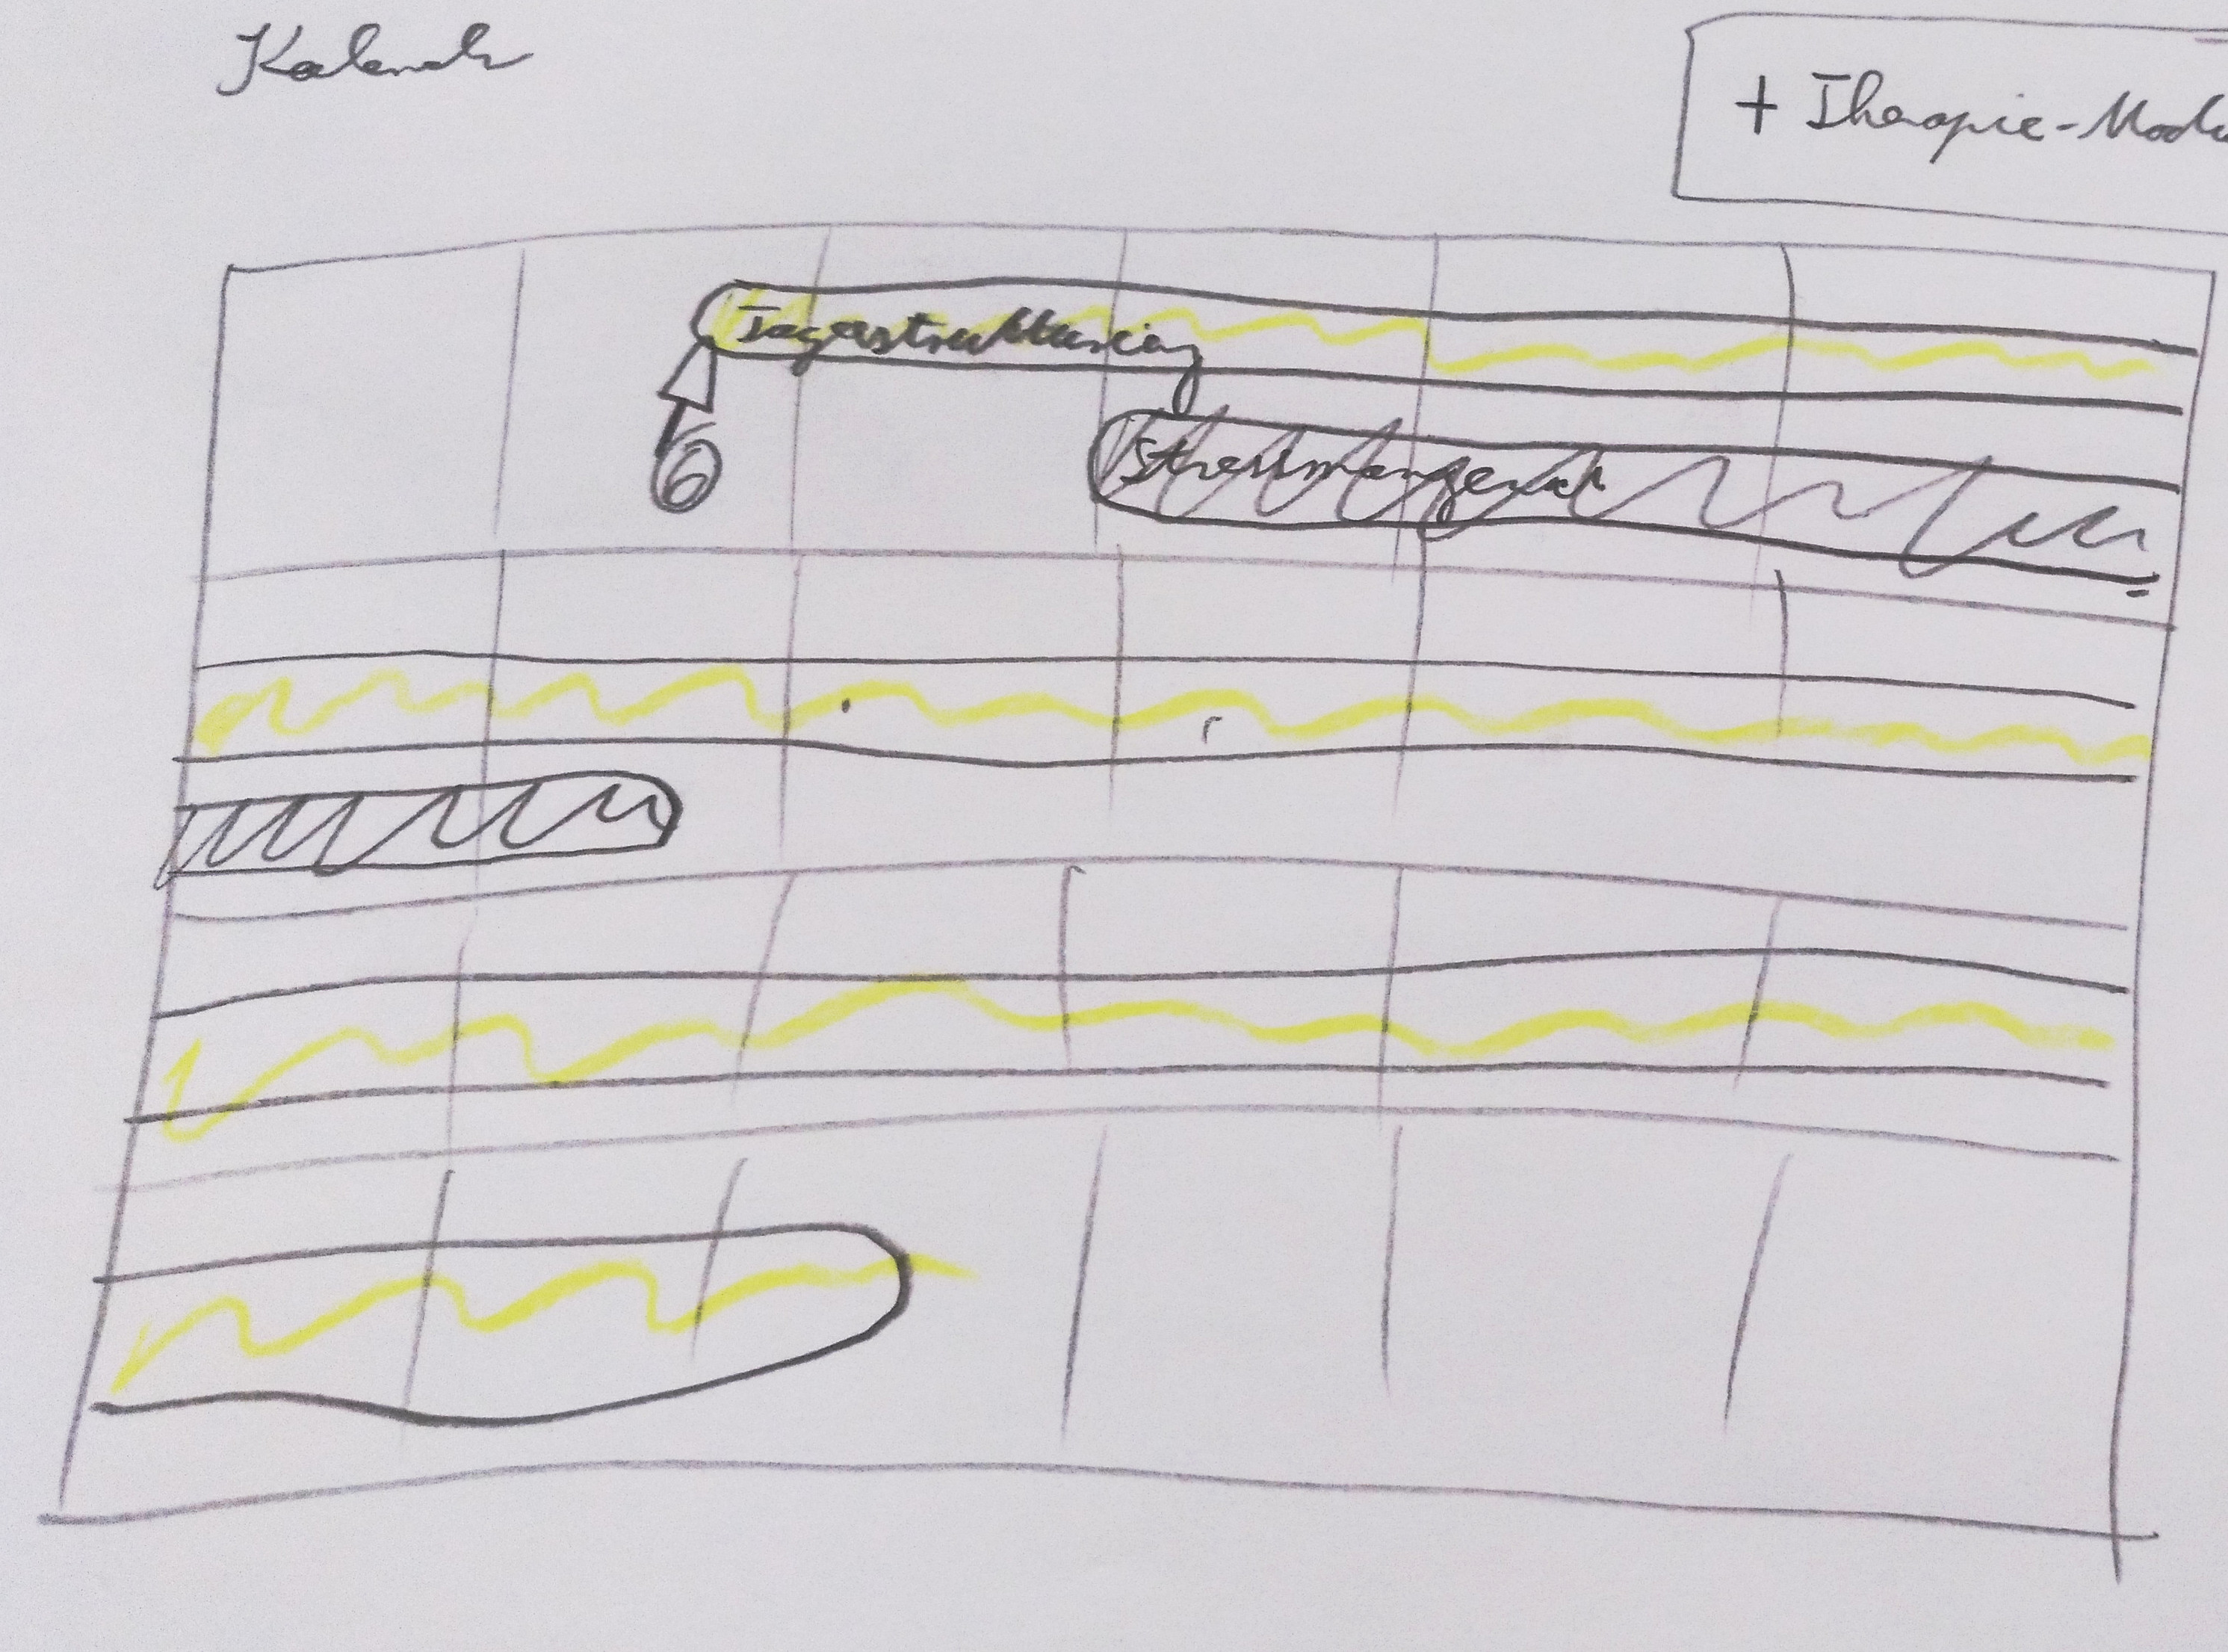
\includegraphics[width=0.75\textwidth]{pictures/moduluebersicht}
\caption{Skizze der zeitlichen Darstellung einzelner Chatbot-Konversationen. Die Darstellung erinnert an ein Gantt-Diagramm.}
\label{moduluebersicht}
\end{figure}

Da hier zunächst noch keine Trigger-Einstellungen erkennbar sind, gibt es einige Überlegungen, diese sichtbar zu machen. Hierfür muss zunächst bedacht werden, welche Form der Trigger-Einstellungen benötigt werden. Diese werden bereits in der zuvor aufgeführten Anforderungsanalyse aufgelistet. Außerdem muss berücksichtigt werden, wie die Trigger vom Forscher eingestellt werden können. Da es sich hierbei um eine Konfiguration handeln soll, die zugleich viel Flexibilität fordert, gibt es die Überlegung, die Konfiguration aus dem Experience-Sampling Tool \emph{movisensXS} zu übersetzen. Das Konstruktionsprinzip des \emph{movisensXS} bietet die Möglichkeit, Trigger, Bedingungen und die anschließend auszuführenden Konversationen, anhand von Blöcken zu verschalten. So können beliebig viele Kombinationen erstellt werden. Dieser Ansatz ist bei steigender Komplexität allerdings unübersichtlich. Abbildung \ref{triggersetkons} skizziert beispielhaft das in \emph{movisensXS} verwendete Konstruktionsprinzip. Um eine Übersichtlichkeit zu behalten, wird die Schaltmöglichkeiten des Konstruktionsprinzip in eine Konfiguration übersetzt. Im \emph{movisensXS} wird unter anderem zwischen Trigger, Bedingungen und Konversationen unterschieden. Zusammengefasst werden diese unter dem Begriff \emph{Time}. Um die Komplexität zu reduzieren und die Einstellungen im Zeitstrahl abzubilden, werden die Trigger und Bedingungen des \emph{movisensXS} direkt auf eine Konversation bezogen, statt Trigger auf mehrere Konversationen anzuwenden. Die aufgelisteten Konversationen erhalten mehrere Einstellungs- und Bearbeitungsmöglichkeiten. Eine dieser Möglichkeiten führt zu den Inhalten der Chatbot-Konversation. Dort wird der Nachrichtenverlauf angelegt und bearbeitet. Eine weitere Möglichkeit ruft den Bearbeitungsdialog der Trigger-Einstellungen der entsprechenden Konversation auf. Auf diese Weise entfällt die Übersetzung der Konversation des \emph{movisensXS}. Das \emph{movisensXS} nutzt Regeln, die den Aufbau des Sampling-Baums bestimmen. Für die Übersetzung der Trigger und Bedingungen werden diese Regeln übertragen. Die Trigger im \emph{movisensXS} Sampling-Baum folgen in der Konfiguration immer als erstes. Diese geben vor, zu welchen Zeiten eine Konversation getriggert werden. Dies wird für das Konstruktionsprinzip übernommen. Zunächst folgen die Trigger-Einstellungen. Ein Trigger muss konfiguriert werden. Dieser gibt zum einen an, durch wen oder was und an welchen Tagen die die Konversation getriggert wird. Soll eine Konversation einem Patienten zwischen Start und Ende dauerhaft zur Verfügung stehen, so kann die Konversation als \emph{Toolbox}-Item markiert werden.  Innerhalb eines Triggers können mehrere Bedingungen angelegt werden. Hier kann beispielsweise nach Variablen-Werten abgefragt werden oder nach dem Zustand einer anderen Konversation. Hierdurch entstehen Abhängigkeiten zwischen Konversationen. Die Bedingungen können beliebig erweitert werden. Da eine Konversation durch mehrere Trigger gestartet werden kann, ist es möglich weitere Trigger anzulegen. Die Abbildung \ref{triggerset} verdeutlicht das Konzept. Tritt somit einer der hinzugefügten Trigger ein, wird die zugehörige Konversation gestartet.

\begin{figure}
   \begin{minipage}[b]{.65\linewidth} % [b] => Ausrichtung an \caption
      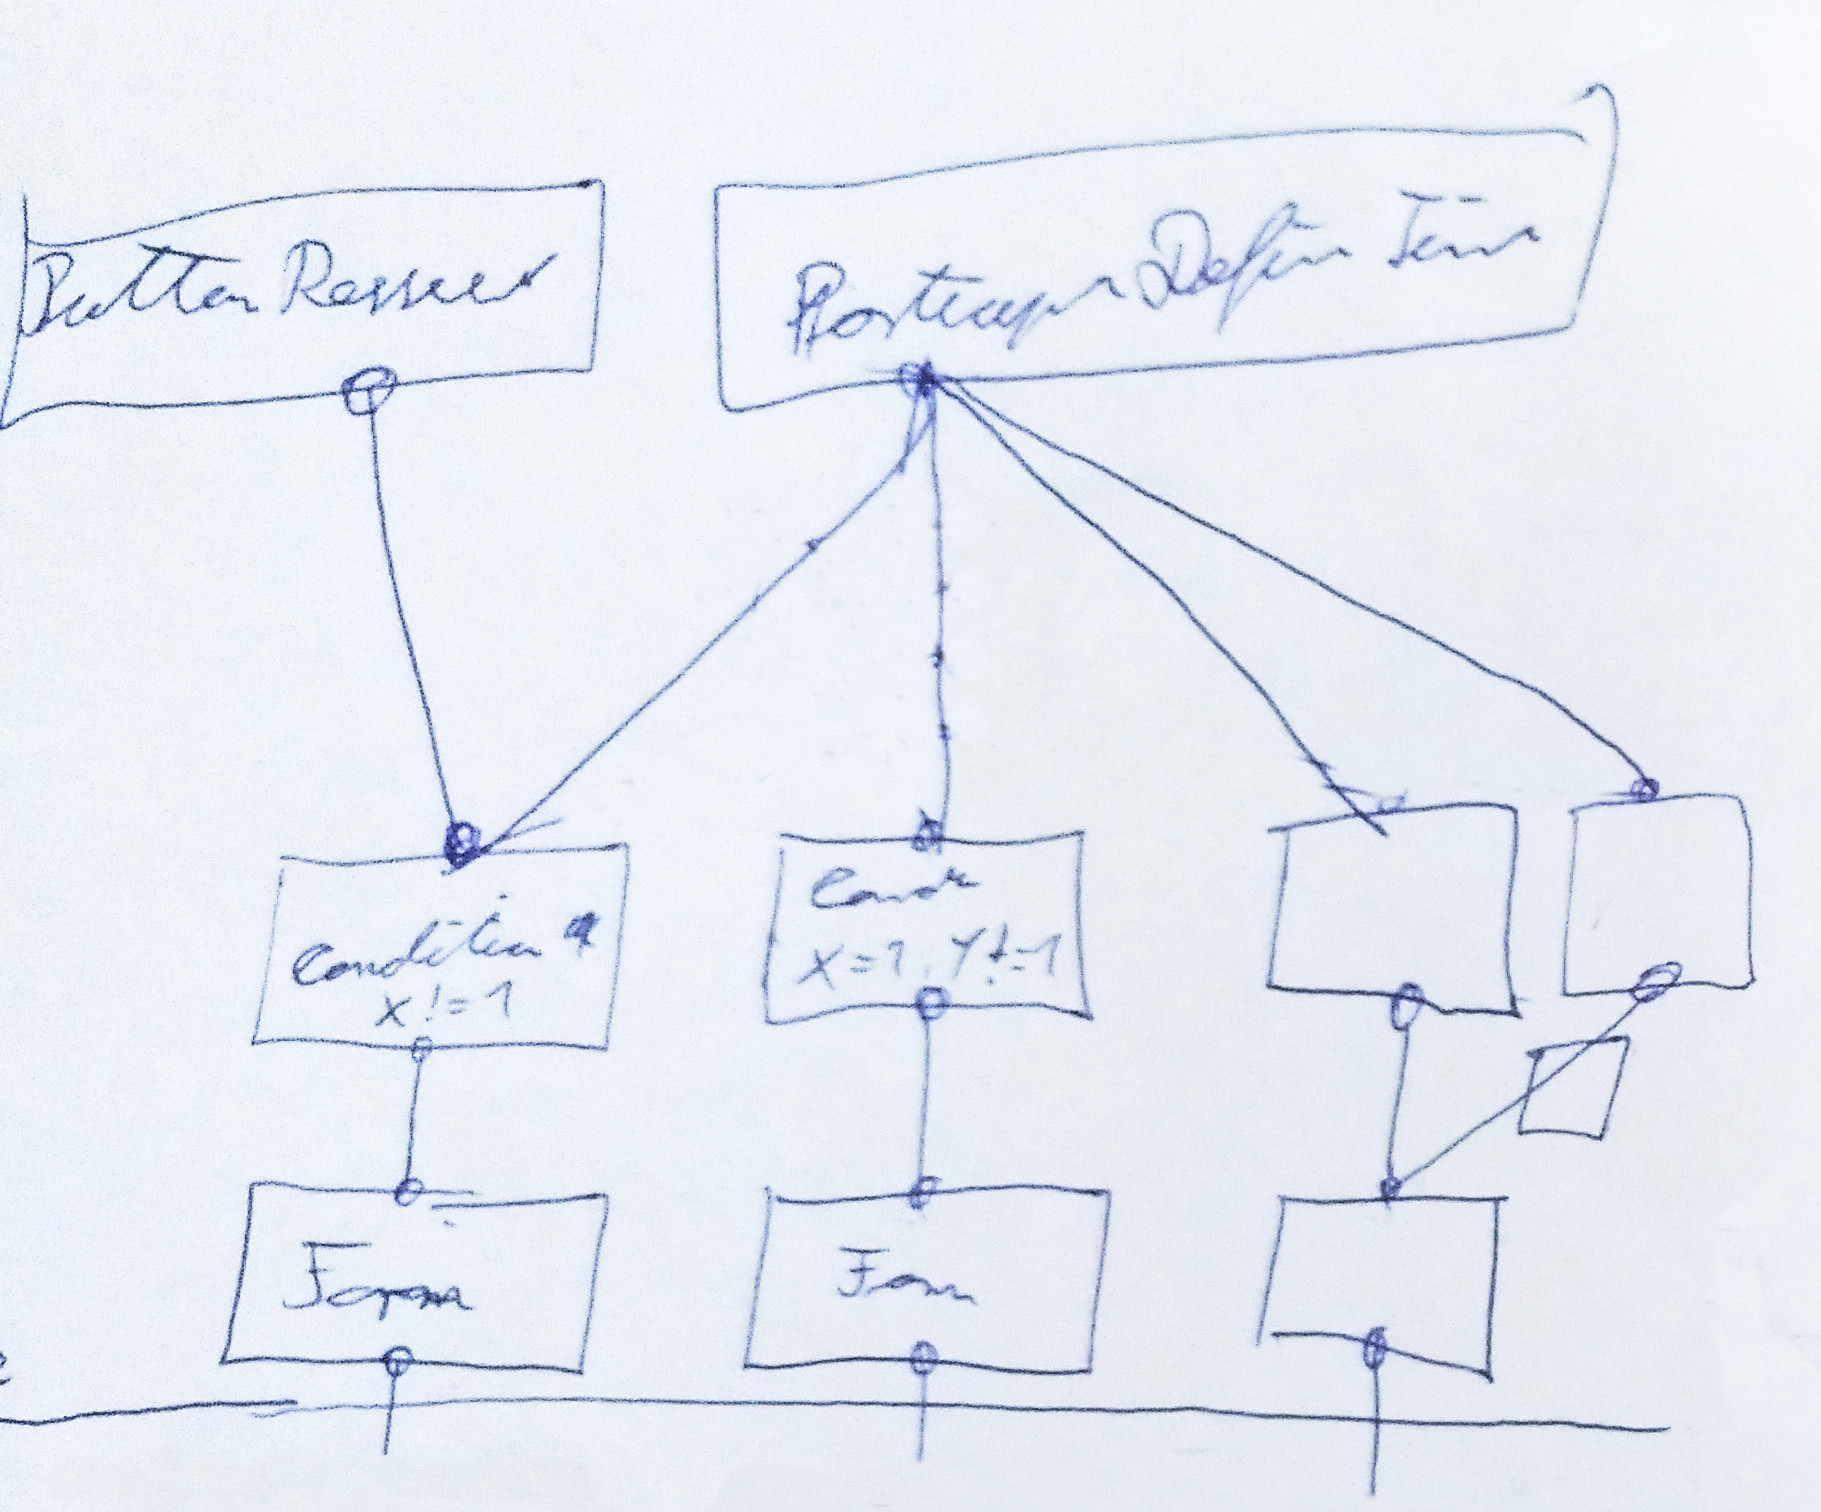
\includegraphics[width=\linewidth]{pictures/triggersetkons}
      \caption{Skizze des Konstruktionsprinzips aus \emph{movisensXS}. Die Anordnung der Trigger ist flexibel. Diese wurde in das Konstruktionsprinzip übersetzt.}
      \label{triggersetkons}
   \end{minipage}
   \hspace{.01\linewidth}% Abstand zwischen Bilder
   \begin{minipage}[b]{.325\linewidth} % [b] => Ausrichtung an \caption
      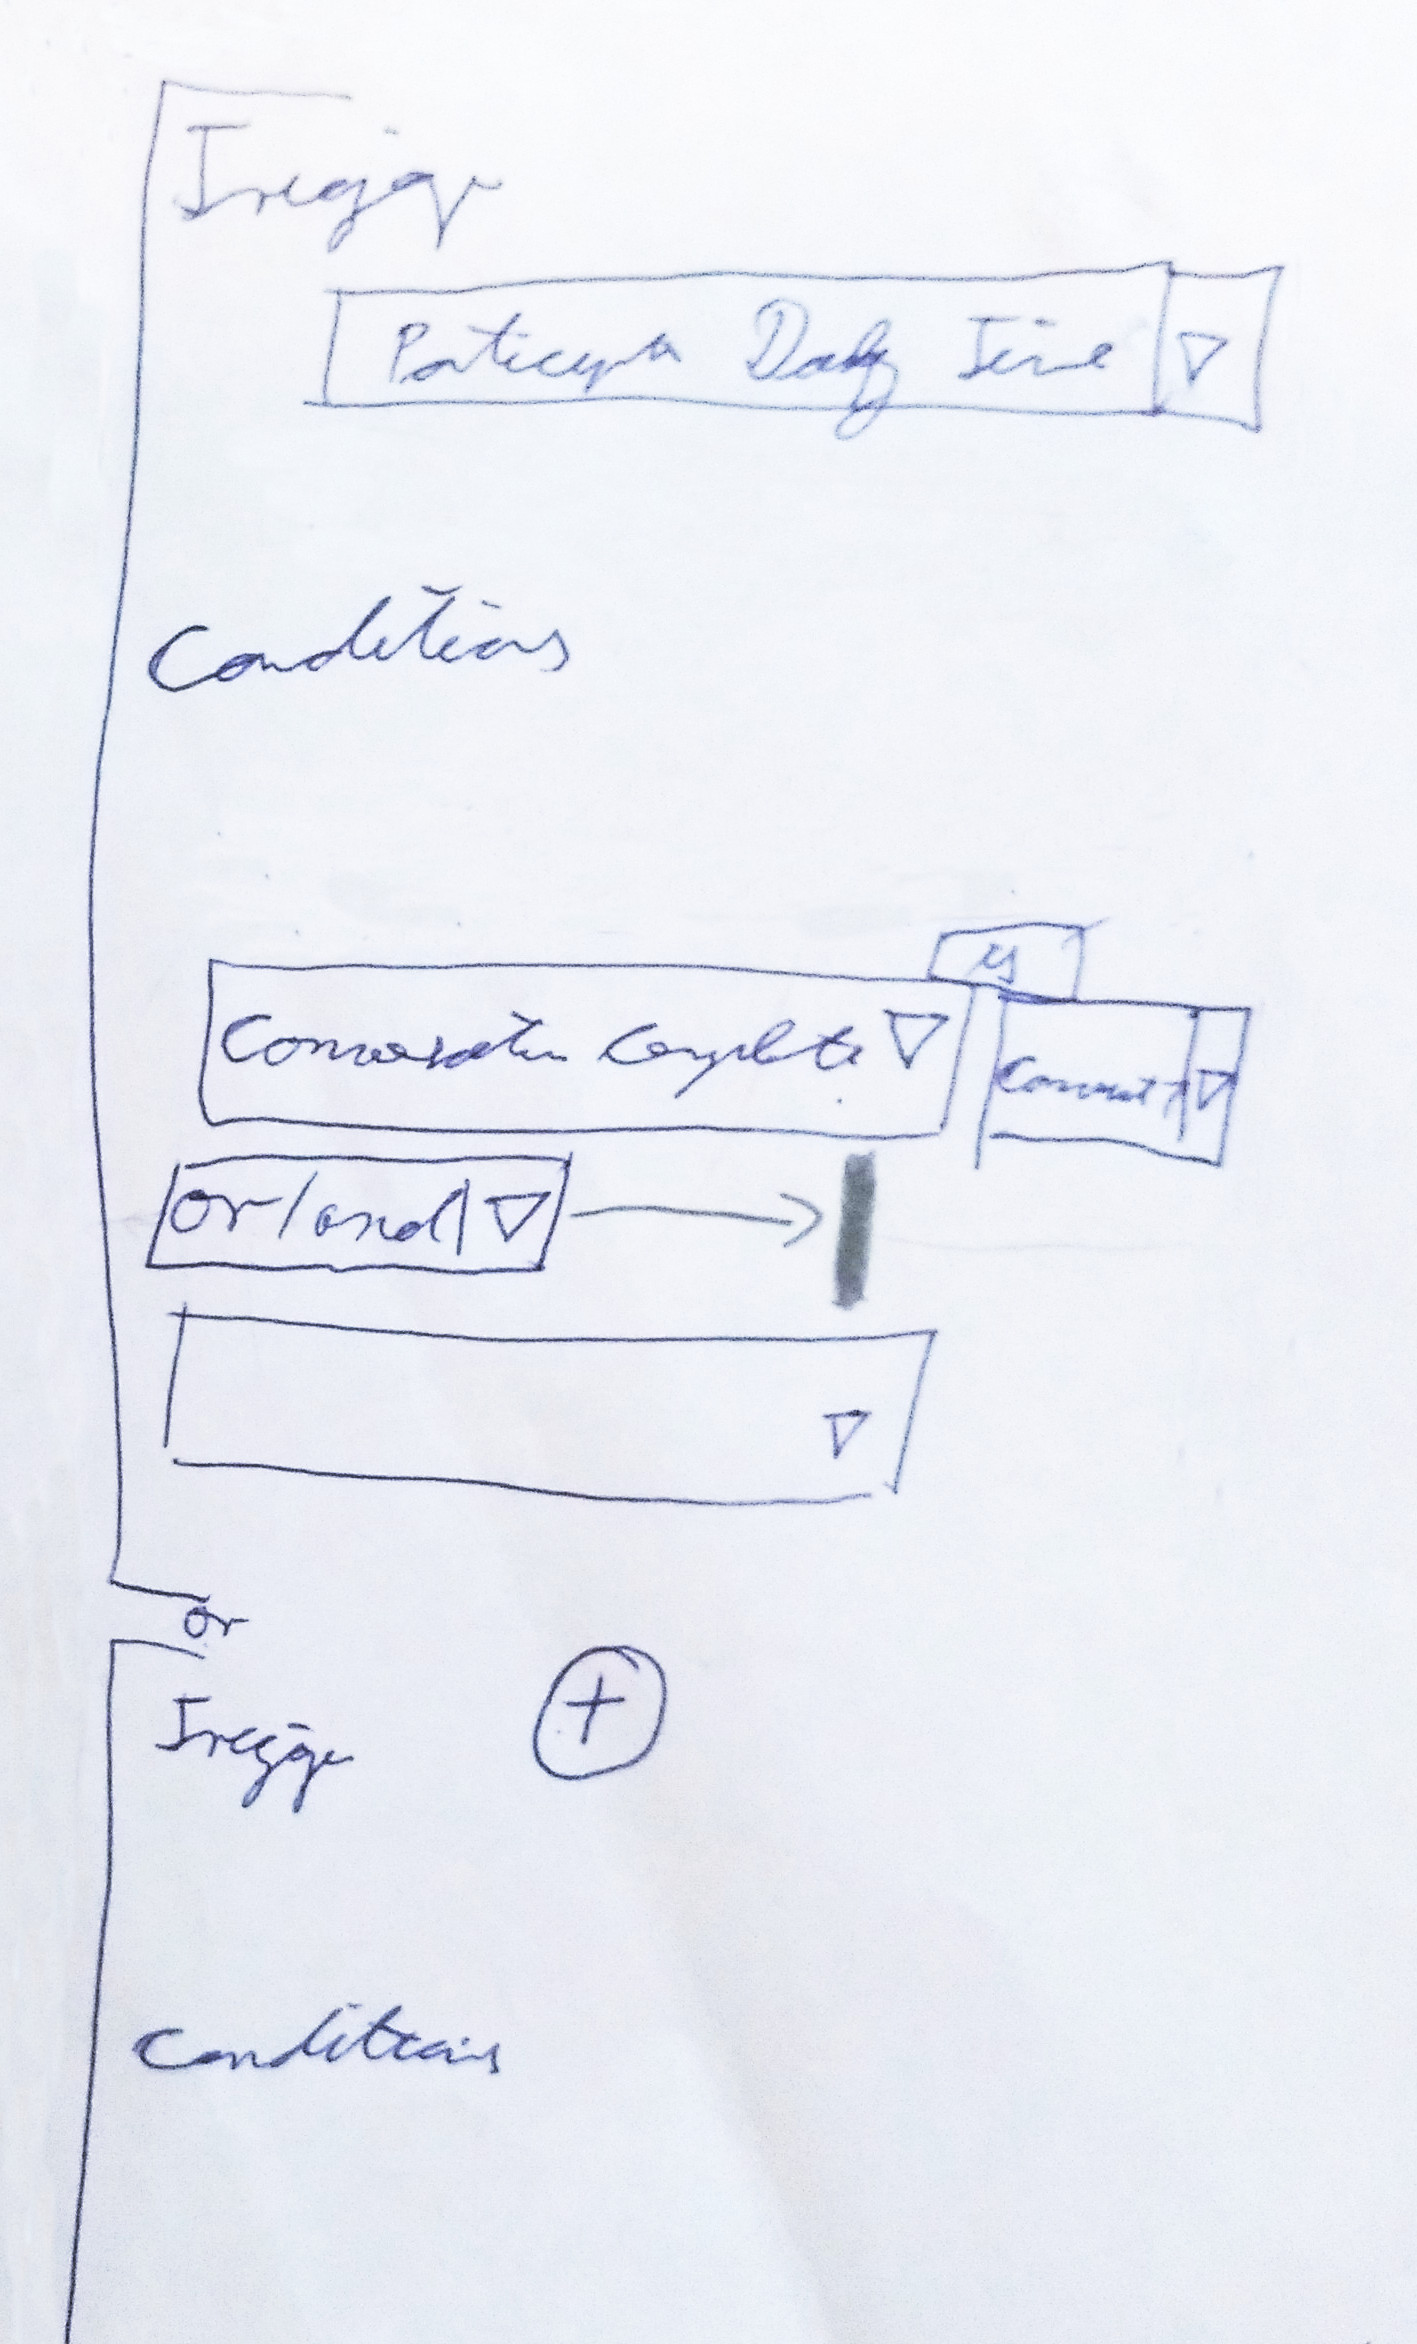
\includegraphics[width=\linewidth]{pictures/triggerset}
      \caption{Die Übersetzung der flexiblen Trigger-Konfiguration.}
      \label{triggerset}
   \end{minipage}
\end{figure}

Diese Vorgaben können nun im Zeitstrahl abgebildet werden. Abhängigkeiten, Toolbox-Items und einfache Konversationen, die keine Abhängigkeiten besitzen, werden farblich Kodiert. Konversationen, die durch den Therapeut, zeitliche Vorgabe des Patienten, oder durch eine andere Konversation gestartet werden, erhalten aussagekräftige Icons. Abhängigkeiten zwischen Konversationen werden im Zeitstrahl durch Linien dargestellt. Die Linien führen von der Konversation, die eine bestimmte Bedingung erfüllen muss, zur Konversation, die erst nach Erfüllung der Bedingung ausgeführt werden kann. 

Die Einstellung der Trigger erfolgt in der Liste der Konversationen. Werden die Trigger-Einstellungen einer Konversation geöffnet, so wechselt die Listendarstellung in die Trigger-Ansicht der jeweiligen Konversation. Die Darstellung der Liste wird in Abbildung \ref{liste} skizziert. Die Liste der Konversationen befindet sich links neben dem Zeitstrahl. Jeder Listeneintrag repräsentiert eine Zeile im Zeitstrahl. Die Konversation und ihre entsprechenden Trigger-Einstellungen werden in ihrer entsprechenden Zeile abgebildet. So besteht ein direkter Zusammenhang zwischen visueller Abbildung im Zeitstrahl und der angelegten Konversation. Eine Konversation wird über ein rundes Schaltelement hinzugefügt. Das Schaltelement beinhaltet ein \emph{+} Symbol und ist bekannt aus dem Material-Design von Google (vgl. \cite{Buttonsf61:online}). Die Listendarstellung der Konversationen bietet außerdem eine Suche. Dies soll das Suchen einer Konversation vereinfachen sobald die Ansicht komplexer wird. 


\begin{figure}[h]
\centering
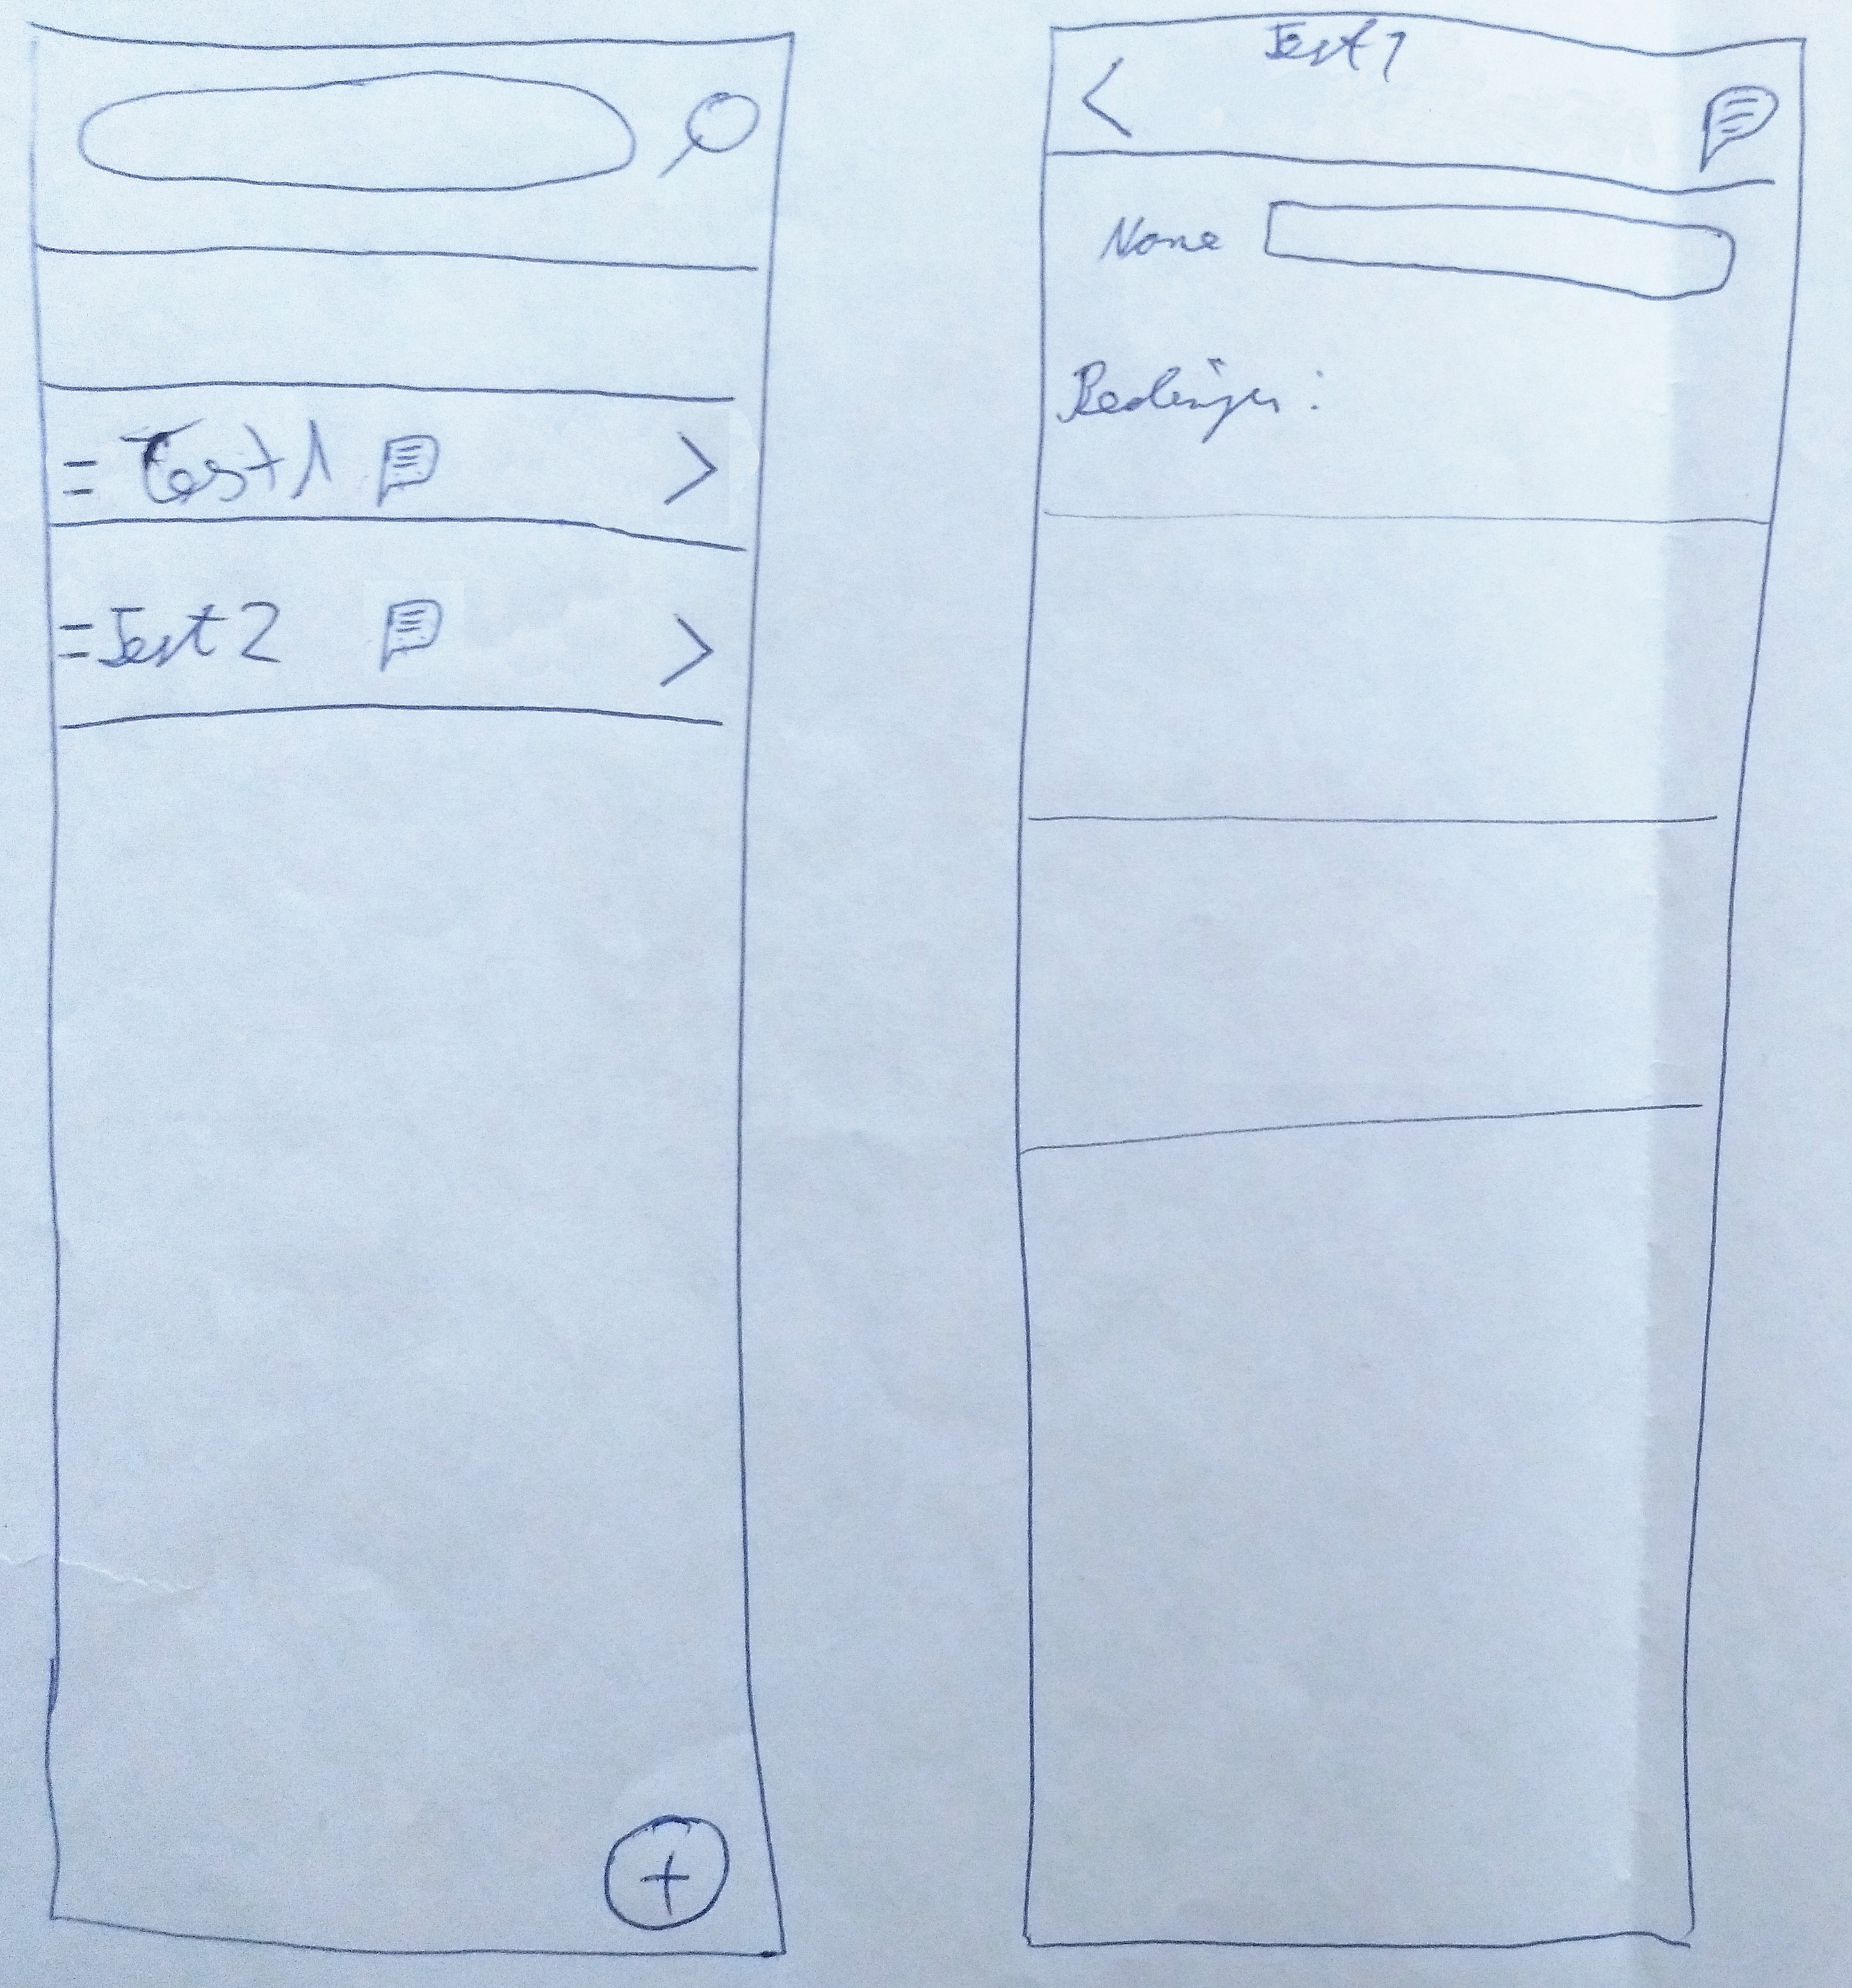
\includegraphics[width=0.5\textwidth]{pictures/liste}
\caption{Skizze einer Liste der Konversationen. Diese wird links neben dem Zeitstrahl platziert.}
\label{liste}
\end{figure}

\subsubsection{Konfigurationsprinzip}

%
%\begin{figure}[h]
%\centering
%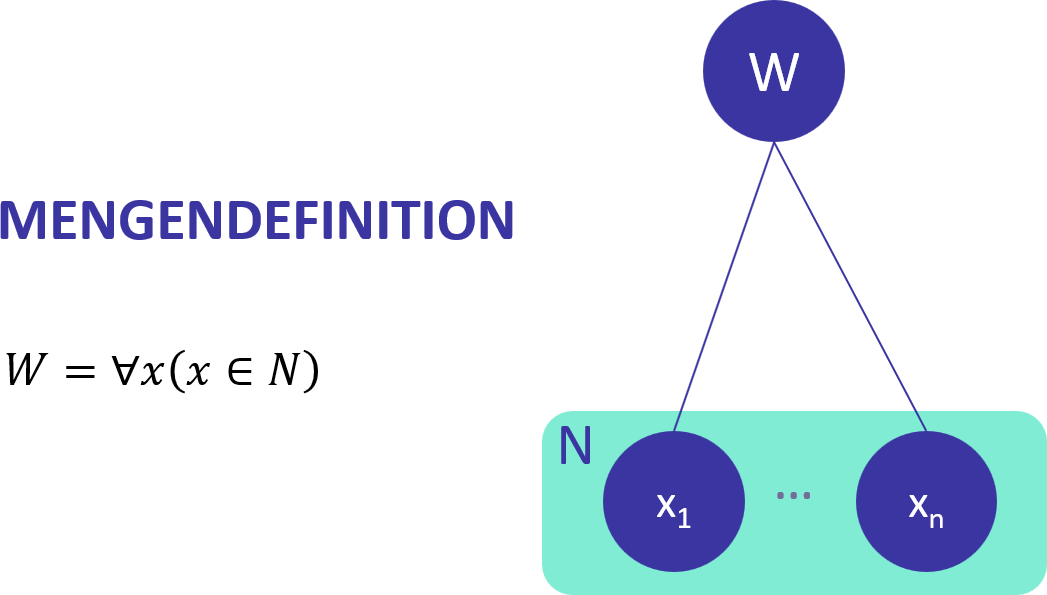
\includegraphics[width=0.5\textwidth]{pictures/toolboxdef}
%\caption{Beziehungen der Mengen}
%\label{therapiedef}
%\end{figure}
     % Konzeption
\chapter{Entwicklung der Modellierungssprache}
\label{ch:Implementation}

\section{Konzept}

\section{Umsetzung}
    % Entwicklung
%% res.tex
%% $Id: eval.tex 5 2005-10-10 20:55:48Z bless $

%%%%%%%%%%%%%
\chapter{Evaluation}
\label{ch:evaluation}
%%%%%%%%%%%%%

\section{Deskriptive Statistik}

\section{Beschreibung der Ergebnisse}

\subsection{Konstruktionsprinzip versus Konfigurationsprinzip}

\subsubsection{Konstruktionsprinzip}
\begin{figure}[h]
\centering
\includegraphics[width=1\textwidth]{pictures/konstruktion}
\caption{Architektur des \emph{konstruktion}}
\label{therapyBuilder}
\end{figure}

\subsubsection{Konfigurationsprinzip}

\begin{figure}[h]
\centering
\includegraphics[width=1\textwidth]{pictures/konfiguration}
\caption{Architektur des \emph{konfiguration}}
\label{therapyBuilder}
\end{figure}


\subsubsection{Gegenüberstellung}


\subsection{Sprünge versus Sichtbarkeitsregeln}

\subsubsection{Sprünge}
\begin{figure}[h]
\centering
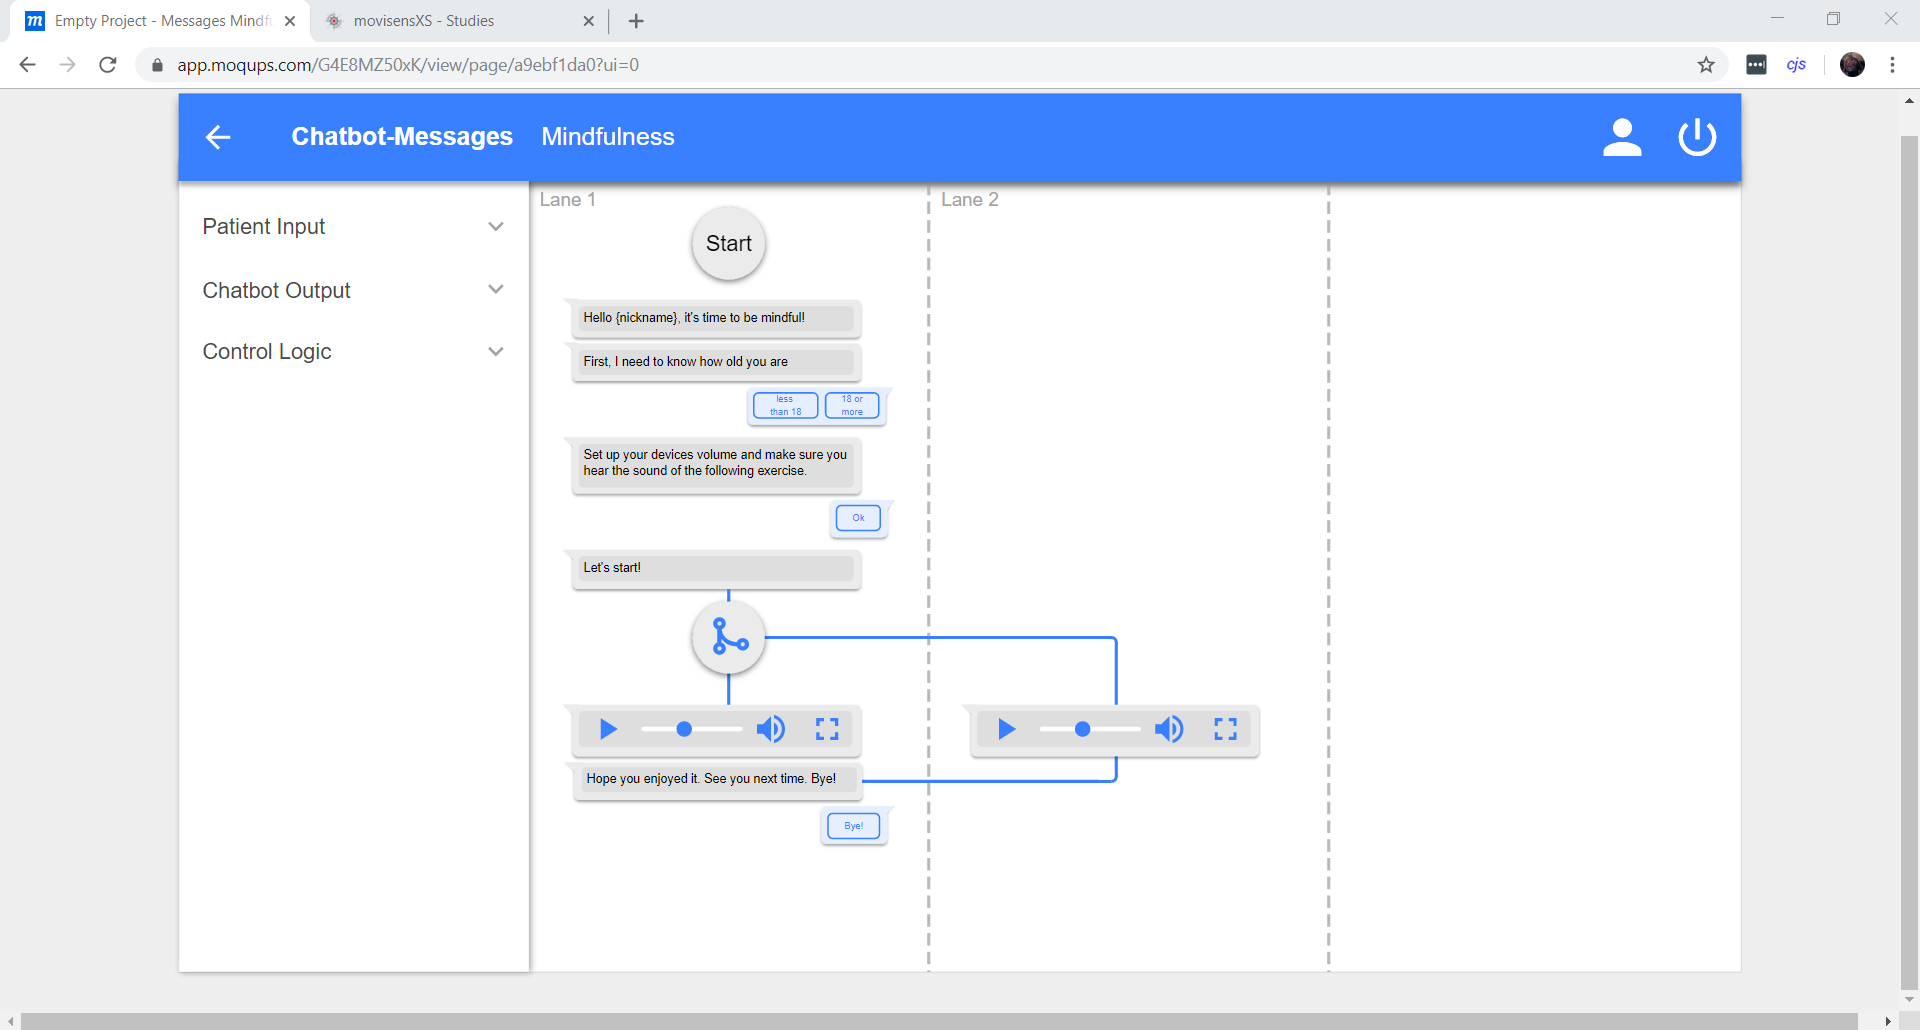
\includegraphics[width=1\textwidth]{pictures/spruenge}
\caption{Architektur des \emph{spruenge}}
\label{therapyBuilder}
\end{figure}


\subsubsection{Sichtbarkeitsregeln}

\begin{figure}[h]
\centering
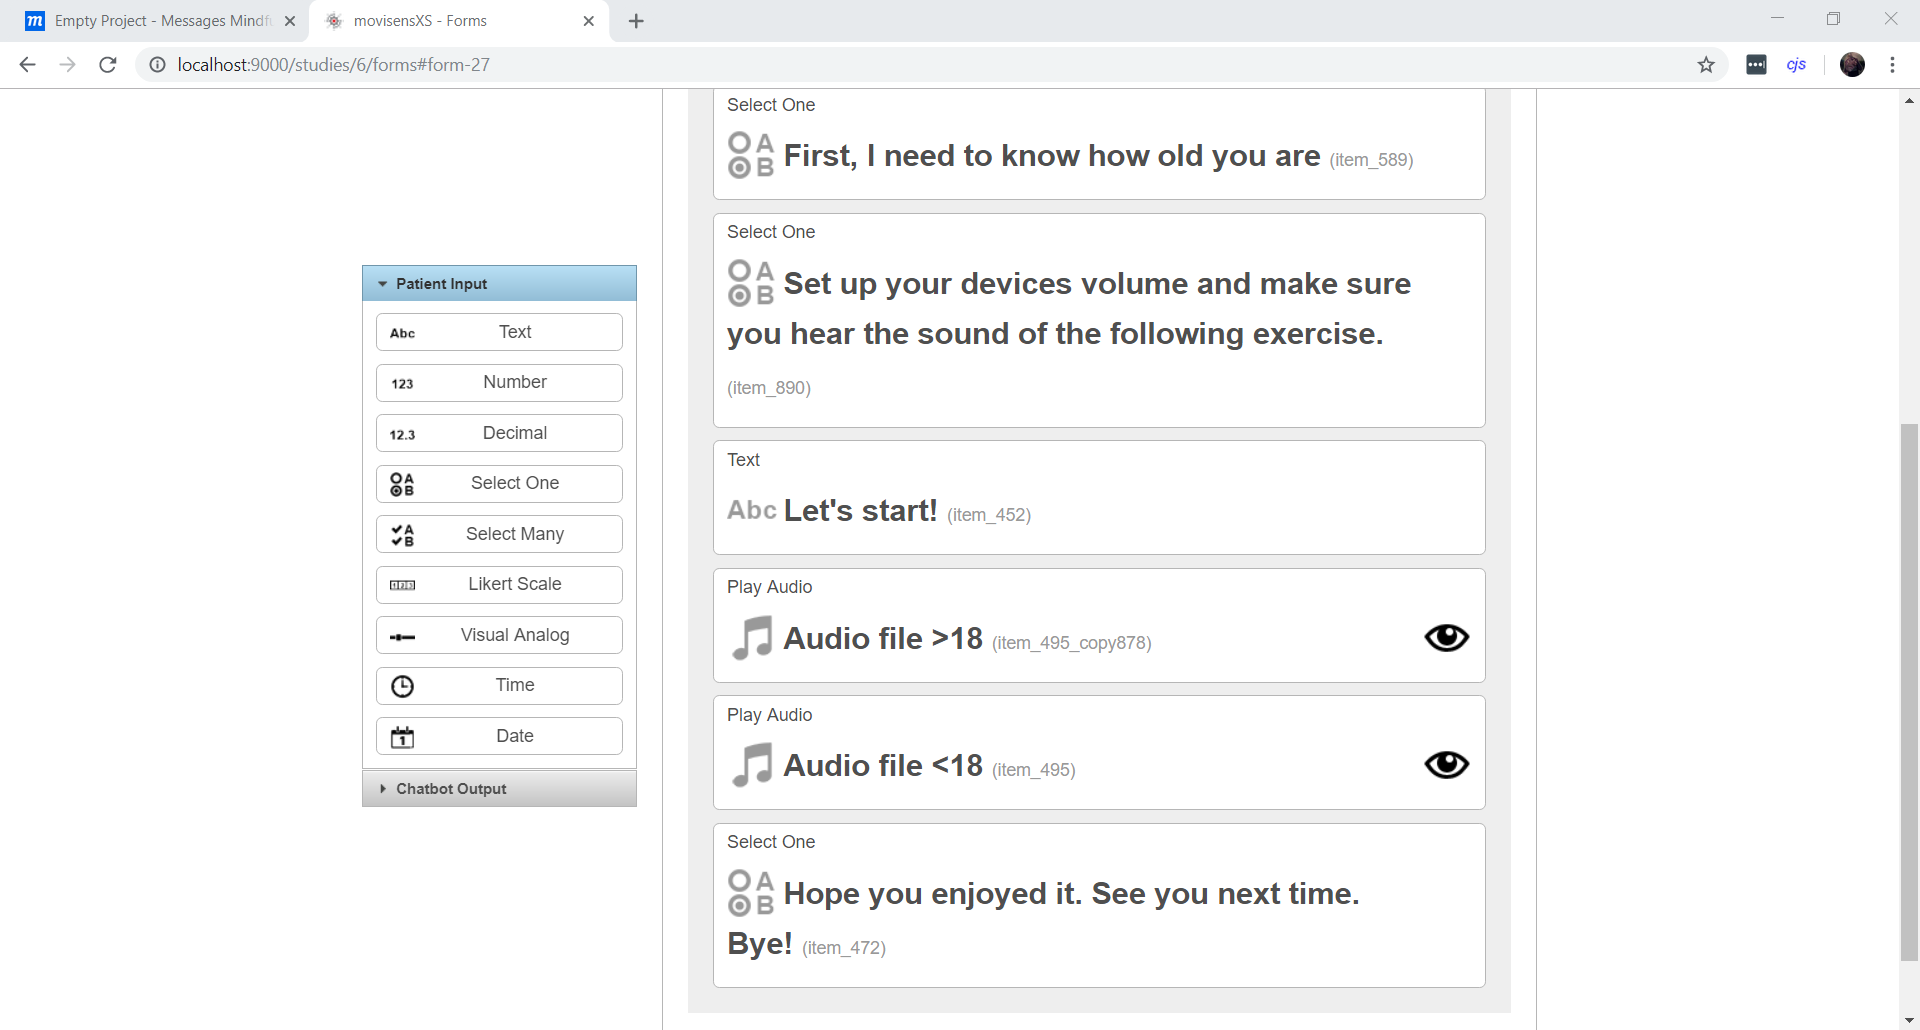
\includegraphics[width=1\textwidth]{pictures/sichtbarkeit}
\caption{Architektur des \emph{sichtbarkeit}}
\label{therapyBuilder}
\end{figure}


\subsubsection{Gegenüberstellung}

\begin{figure}[h]
\centering
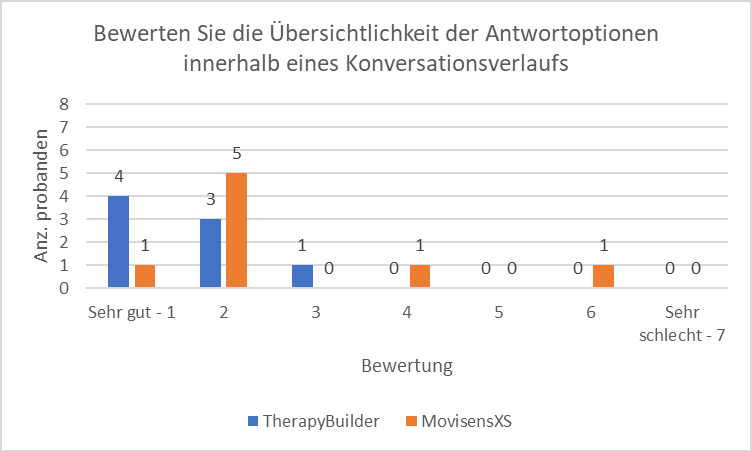
\includegraphics[width=1\textwidth]{pictures/diagramme/antwortoptkonv}
\caption{Architektur des \emph{sichtbarkeit}}
\label{therapyBuilder}
\end{figure}

\begin{figure}[h]
\centering
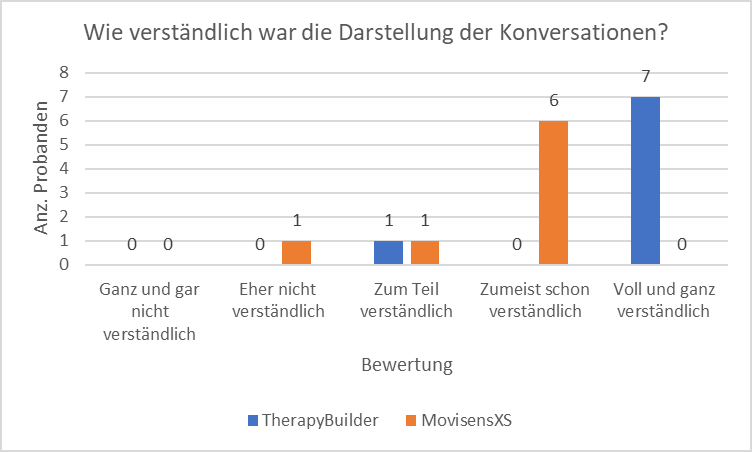
\includegraphics[width=1\textwidth]{pictures/diagramme/konversationdarstellung}
\caption{Architektur des \emph{konfiguration}}
\label{therapyBuilder}
\end{figure}

\begin{figure}[h]
\centering
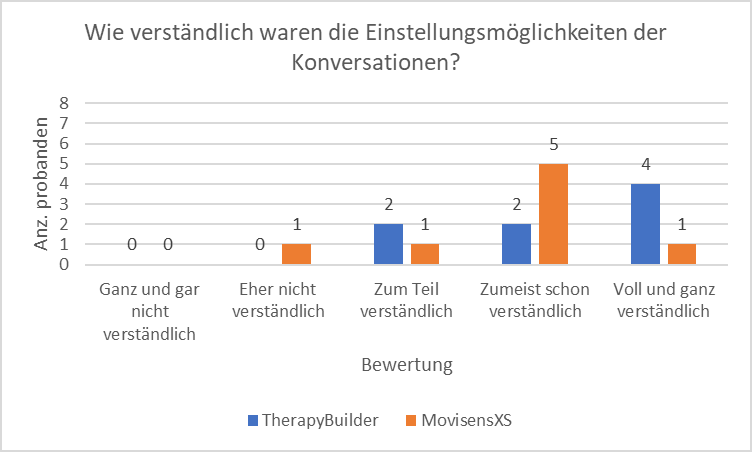
\includegraphics[width=1\textwidth]{pictures/diagramme/konversationeinstellung}
\caption{Architektur des \emph{konfiguration}}
\label{therapyBuilder}
\end{figure}

\begin{figure}[h]
\centering
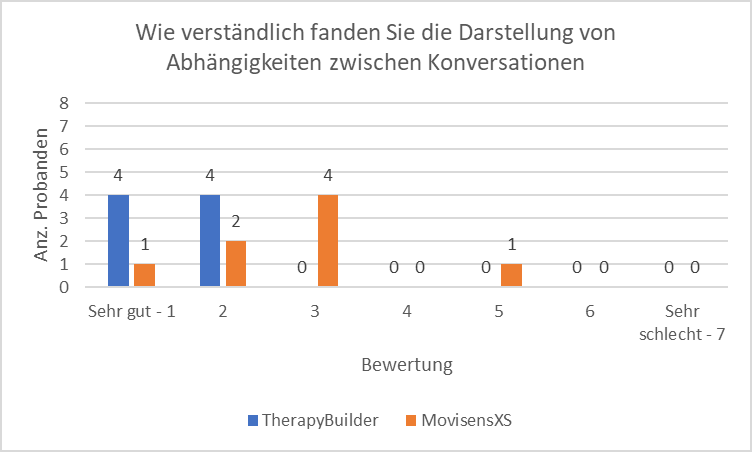
\includegraphics[width=1\textwidth]{pictures/diagramme/konversationenabhaeng}
\caption{Architektur des \emph{konfiguration}}
\label{therapyBuilder}
\end{figure}

\begin{figure}[h]
\centering
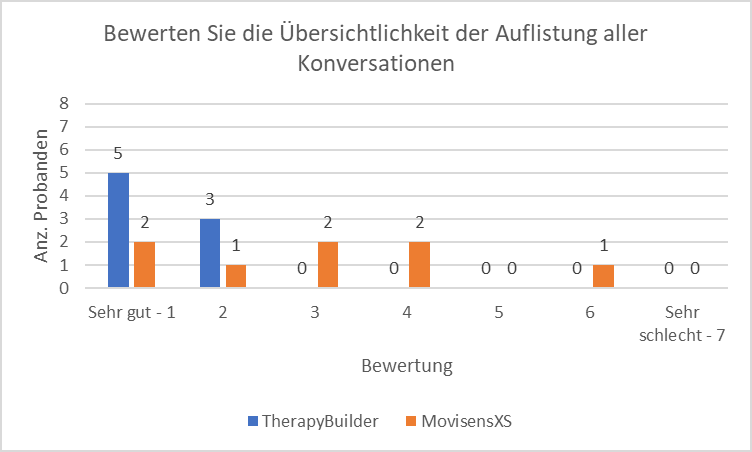
\includegraphics[width=1\textwidth]{pictures/diagramme/konversationenuebersicht}
\caption{Architektur des \emph{konfiguration}}
\label{therapyBuilder}
\end{figure}

\begin{figure}[h]
\centering
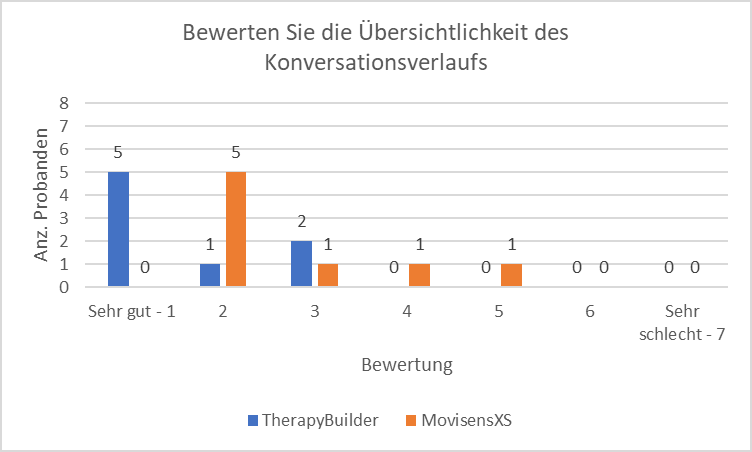
\includegraphics[width=1\textwidth]{pictures/diagramme/konversationverlfueber}
\caption{Architektur des \emph{konfiguration}}
\label{therapyBuilder}
\end{figure}

\begin{figure}[h]
\centering
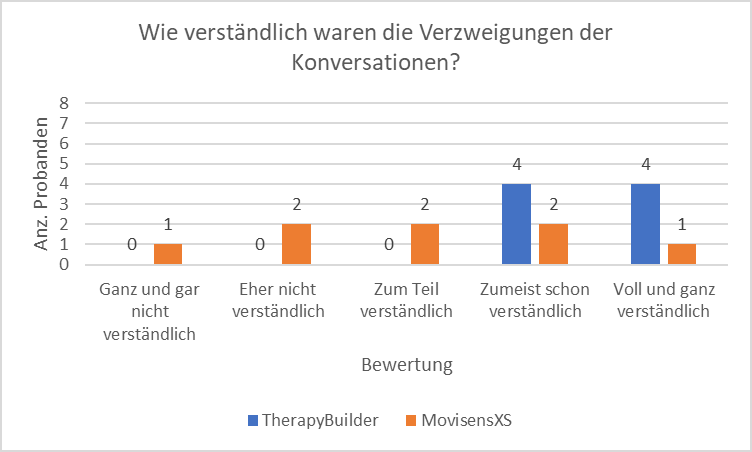
\includegraphics[width=1\textwidth]{pictures/diagramme/konversationverzweigung}
\caption{Architektur des \emph{konfiguration}}
\label{therapyBuilder}
\end{figure}

\begin{figure}[h]
\centering
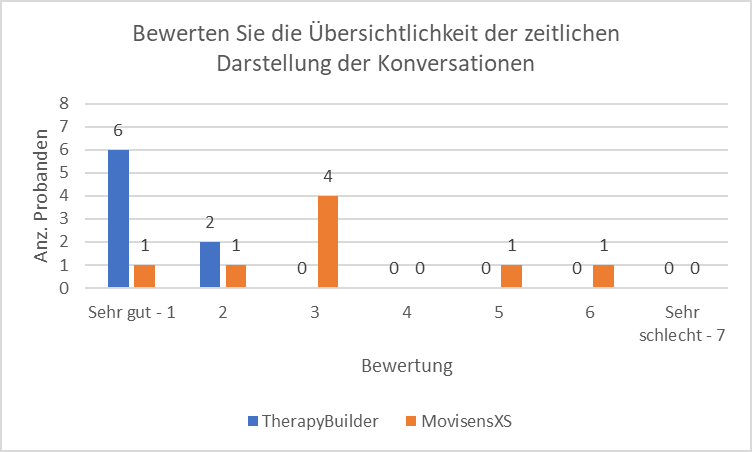
\includegraphics[width=1\textwidth]{pictures/diagramme/konversationzeitldarstellung}
\caption{Architektur des \emph{konfiguration}}
\label{therapyBuilder}
\end{figure}

\begin{figure}[h]
\centering
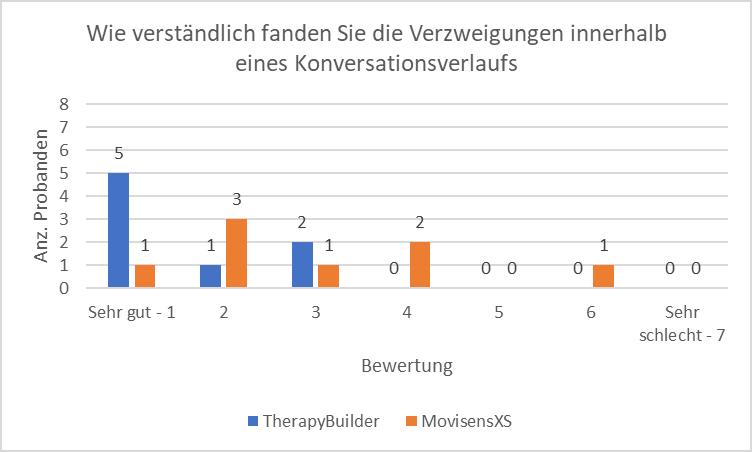
\includegraphics[width=1\textwidth]{pictures/diagramme/konvverzweig}
\caption{Architektur des \emph{konfiguration}}
\label{therapyBuilder}
\end{figure}

\begin{figure}[h]
\centering
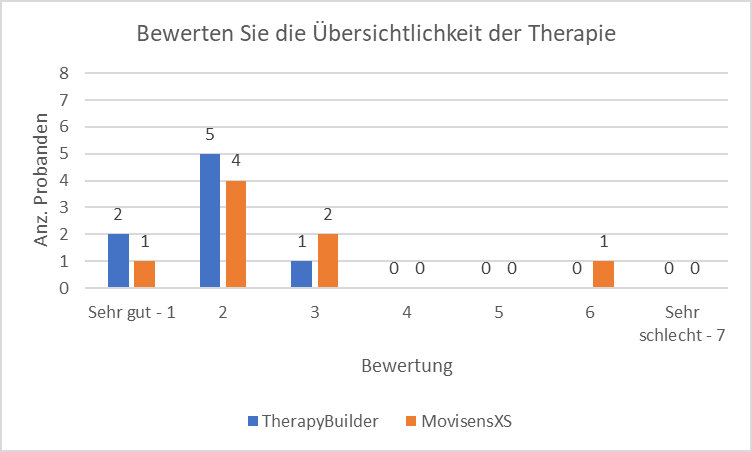
\includegraphics[width=1\textwidth]{pictures/diagramme/therapieuebersicht}
\caption{Architektur des \emph{konfiguration}}
\label{therapyBuilder}
\end{figure}

\begin{figure}[h]
\centering
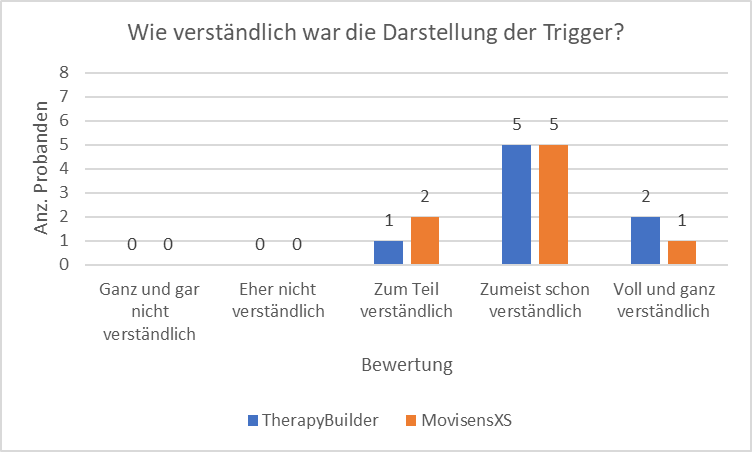
\includegraphics[width=1\textwidth]{pictures/diagramme/triggerdarstellung}
\caption{Architektur des \emph{konfiguration}}
\label{therapyBuilder}
\end{figure}

\begin{figure}[h]
\centering
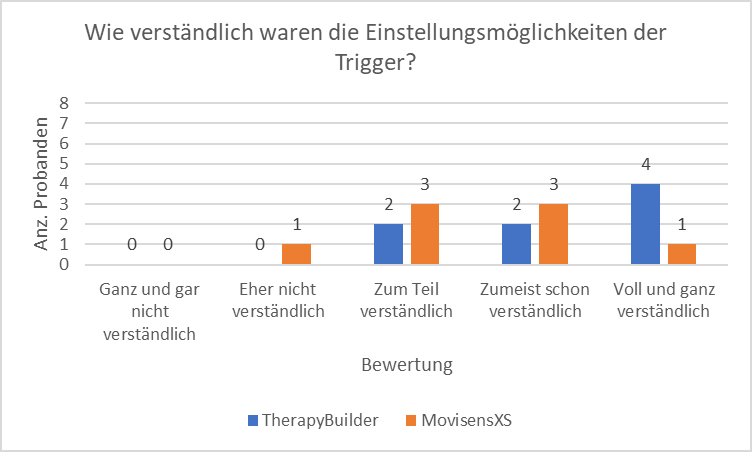
\includegraphics[width=1\textwidth]{pictures/diagramme/triggereinstellung}
\caption{Architektur des \emph{konfiguration}}
\label{therapyBuilder}
\end{figure}

\begin{figure}[h]
\centering
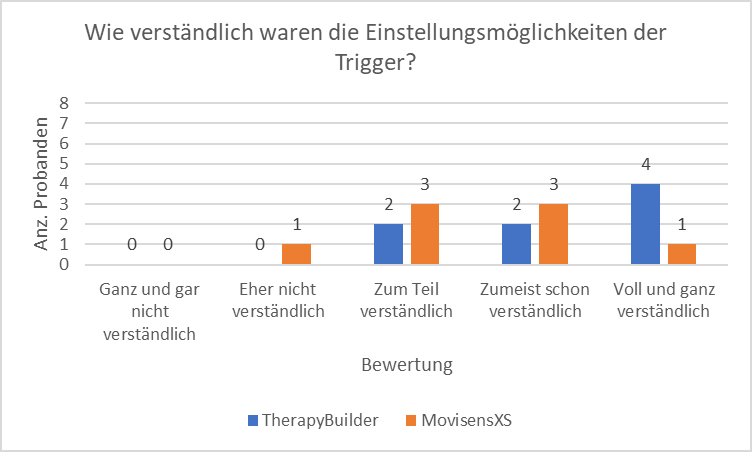
\includegraphics[width=1\textwidth]{pictures/diagramme/triggereinstellung}
\caption{Architektur des \emph{konfiguration}}
\label{therapyBuilder}
\end{figure}

\begin{figure}[h]
\centering
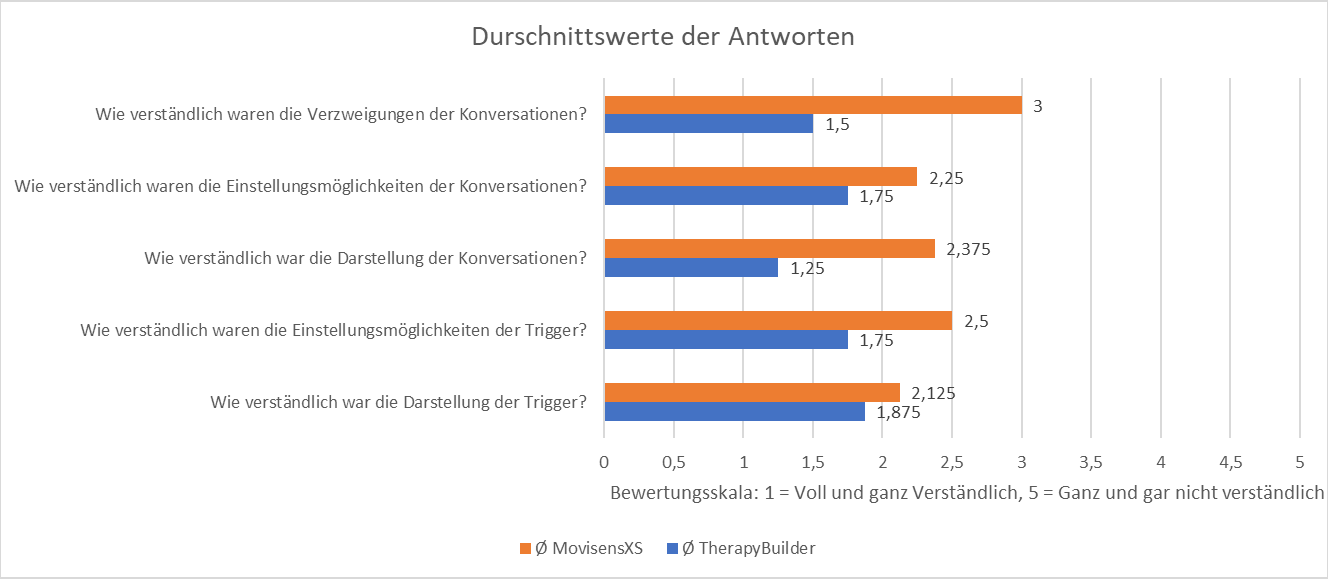
\includegraphics[width=1\textwidth]{pictures/diagramme/antwortendurchsch1}
\caption{Architektur des \emph{konfiguration}}
\label{therapyBuilder}
\end{figure}

\begin{figure}[h]
\centering
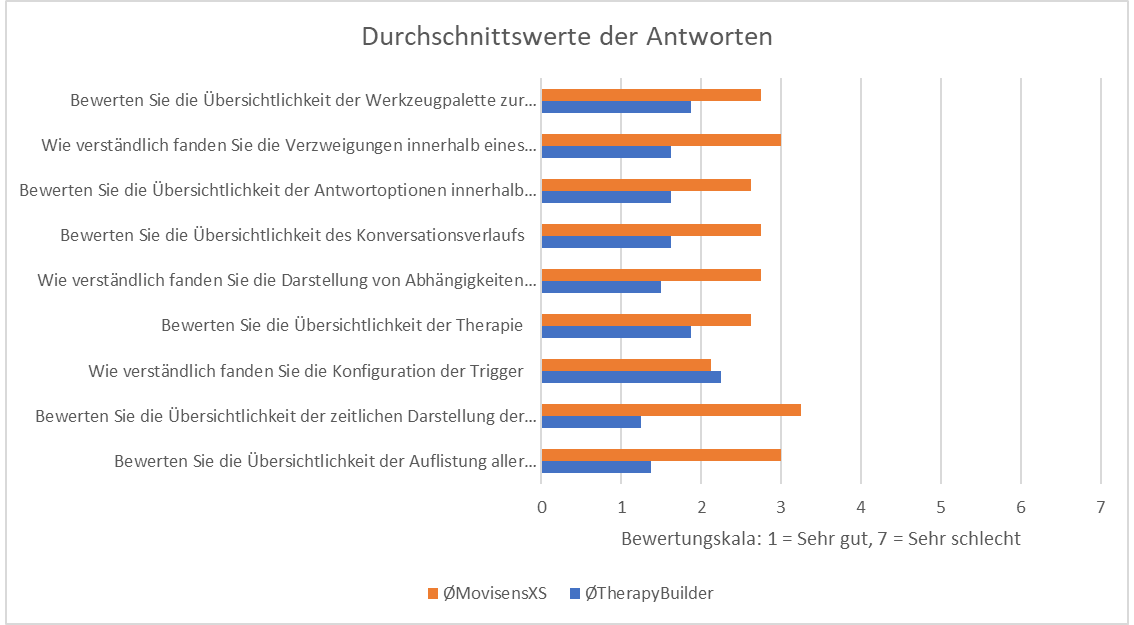
\includegraphics[width=1\textwidth]{pictures/diagramme/antwortendurchsch2}
\caption{Architektur des \emph{konfiguration}}
\label{therapyBuilder}
\end{figure}        % Evaluierung
%%%%%%%%%%%%%
\chapter{Ergebnisdiskussion}
\label{ch:Results}
%%%%%%%%%%%%%
Zur Bewertung der Konzepte werden die in Kapitel \ref{ch:evaluation} beschriebenen Daten zunächst interpretiert. Die Ergebnisse der Interpretation werden anschließend kritisch betrachtet und, basierend auf der Ergebnisinterpretation, ein Ausblick der nächsten Schritte, für die Umsetzung des \emph{TMA} beschrieben. 


\section{Ergebnisinterpretation}
Die Ergebnisinterpretation erfolgt auf den, in Kapitel \ref{ch:evaluation}, aufgestellten Hypothesen. Ziel der Ergebnisinterpretation ist darzulegen, dass ein Modellierungsansatz nach dem Konfigurationsprinzip für den späteren Anwender verständlicher ist. Als Baseline dient hierfür das \emph{movisensXS}-System, welches ein Konstruktionsprinzip verfolgt. Dieser Ansatz bietet im Vergleich sehr viel Flexibilität in der Gestaltung einer Therapie. Die Ergebnisse werden kategorisiert betrachtet. Gegenübergestellt werden jeweils, wie bisher, das Konstruktionsprinzip und Konfigurationsprinzip, sowie der Einsatz von Sprüngen und die Verwendung von Sichtbarkeitsregeln. Die Betrachtung der Ergebnisse wird gemäß der zuvor verwendeten Reihenfolge erfolgen. Abschließend werden die Ergebnisse zusammengefasst dargestellt.


\subsection{Konfigurationsprinzip und Konstruktionsprinzip}
Eine erste Betrachtung der Ergebnisse, deutet darauf hin, dass die Nutzer die Umsetzung und Verwendung des Konfigurationsprinzips besser bewerteten als das Konstruktionsprinzip. Wie in Abbildung \ref{antwortendurchsch11} und Abbildung \ref{antwortendurchsch22} zu sehen ist, haben die Probanden den \emph{TherapyBuilder}-Prototyp im Schnitt besser bewertet als das angepasste \emph{movisensXS}-System. Diese Ergebnisse wurden den Zwischenfragebögen entnommen und zeigen eine erste Tendenz auf. 

Auch die Ergebnisse der Abschlussfragerunde geben einen ersten Hinweis auf die Bewertung der Verständlichkeit und Übersicht beider Prinzipien. Insgesamt konnten die Probanden in der Abschlussfragerunde achtundzwanzig Punkte nennen (vgl. Abbildung \ref{konstrabsch} und \ref{konfigabsch}), die ihnen am Konstruktionsprinzip gut gefallen haben und die sie besonders hilfreich empfanden. Zum Konfigurationsprinzip äußerten sie hierzu hingegen neununddreißig Punkte. Die Probanden konnten somit bezüglich des Konfigurationsprinzips insgesamt mehr Punkte äußern, die ihnen an dieser Umsetzung gut gefallen haben und besonders hilfreich empfunden wurden. Betrachtet man diese jedoch im Einzelnen, wurden Konstruktionsprinzip mehr Punkte dahingehend geäußert, was den Probanden gut gefallen hat. Hinsichtlich der Nachfrage, was den Probanden an der jeweiligen Umsetzung nicht gefallen hat und was sie vermisst haben, schnitt auch hier das Konfigurationsprinzip besser ab. Im Vergleich zum Konstruktionsprinzip fielen den Probanden neunzehn Punkte ein. Das sind dreizehn Punkte weniger als die Probanden zum Konstruktionsprinzip äußerten. Zwar gibt es insgesamt mehr positive Anmerkungen bezüglich des Konfigurationsprinzip, allerdings wurden gegenüber dem Konstruktionsansatz mehr Punkte genannt, die den Probanden an diesem Ansatz besonders gut gefallen haben. Welche Punkte das sind und wie sich diese mit den Ergebnissen und aufgestellten Hypothesen verbinden lassen, wird im Verlauf dieses Kapitels betrachtet.


\begin{figure}
   \begin{minipage}[b]{.49\linewidth} % [b] => Ausrichtung an \caption
      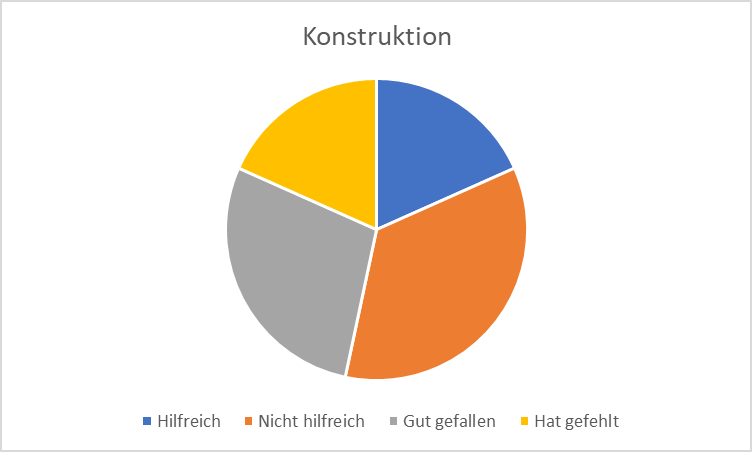
\includegraphics[width=\linewidth]{pictures/diagramme/aussagenkonstr}
      \caption{Zu sehen ist die Anzahl der genannten Punkte der Abschlussfragerunde. Die Probanden nannten achtundzwanzig Punkte auf die Frage was ihnen am Konstruktionsprinzip gut gefällt und sie als hilfreich empfinden}
      \label{konstrabsch}
   \end{minipage}
   \hspace{.01\linewidth}% Abstand zwischen Bilder
   \begin{minipage}[b]{.49\linewidth} % [b] => Ausrichtung an \caption
      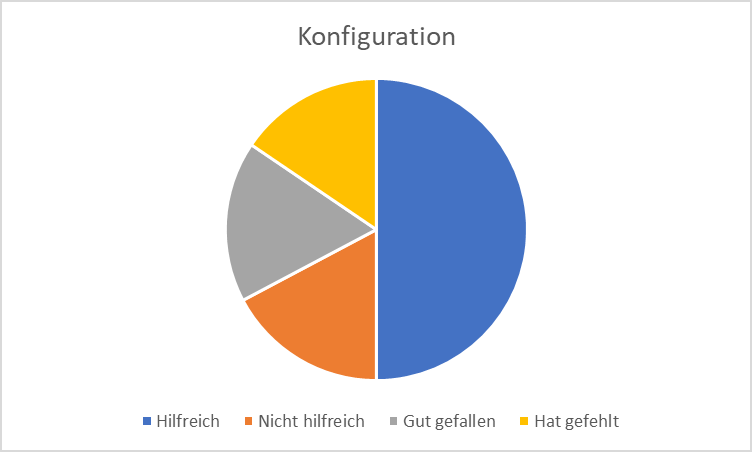
\includegraphics[width=\linewidth]{pictures/diagramme/aussagenkonfig}
      \caption{Im Vergleich äußerten die Probanden deutlich mehr Punkte, die sie am umgesetzten Konfigurationsprinzip als hilfreich empfinden. Allerdings konnten sie auch weniger Aussagen darüber treffen, was ihnen besonders gut gefallen hat}
      \label{konfigabsch}
   \end{minipage}
\end{figure}



\paragraph{Verständlichkeit der Triggereinstellungen}
Die Ergebnisse der Zwischenfragebögen zeigen eine Tendenz, dass im Vergleich das Kontruktionsprinzip für Anwender verständlicher ist. Die Freitexte der Zwischenfragebögen und Abschlussfragerunde deuten hingegen darauf hin, dass zwar viele Einstellungsmöglichkeiten geboten werden ohne mit diesen zu erschlagen und gefühlt weniger Einstellungsschritte und notwendig sind. Der Fluss vom Klicken wirkt klarer und konsistenter. Allerdings äußerten mehrere Probanden, dass die Einstellungen der Trigger zunächst irritierten. Betrachtet man die Ergebnisse der Abschlussfragerunde bestätigt sich letztere Aussage. Die Hälfte der Probanden wünschen sich eine Anleitung oder Tooltips zum besseren Verständnis der Triggereinstellungen.

Zwar wurde das \emph{movisensXS}-System im Zwischenfragebogen hinsichtlich der Triggereinstellungen schlechter bewertet. Dennoch kann das verwendete Konstruktionsprinzip mit seiner flexiblen Gestaltungsmöglichkeit aufwarten. Die Einstellungen der Trigger werden bei wachsender Komplexität unübersichtlicher. Aber insbesondere die vielen Einstellungsmöglichkeiten via Drag and Drop durch das Baukastenprinzip, und die Flexibilität in der Anordnung und Gestaltung, sind generell besser nachvollziehbar. Nicht nur das Baukastenprinzip und die einhergehende Drag and Drop Funktion tragen dazu bei, sondernm auch die Trennung verschiedener Elemente anhand ihrer Funktion. 

Insgesamt ist zwar eine Tendenz gegeben, dass das Konstruktionsprinzip leichter verständlich ist, allerdings benötigt dieses zusätzlich Anleitungen und Tooltips um diese zu verbessern. Auch wenn das Konstruktionsprinzip tendenziell schlechter abschneidet, so ist gerade das zusammenbauen der Triggereinstellungen für die Nutzer interessant und das Prinzip an sich leicht nachvollziehbar. Allerdings kann hier auch die flexible Anordnung zu einer geringeren Übersicht beitragen. Hier könnte eine automatische Anordnungsfunktion, oder Anordnungshilfe zur besseren Übersicht beitragen.


\paragraph{Verständlichkeit der Triggerdarstellung}
Auch hier lässt sich in Abbildung \ref{antwortendurchsch1} eine leichte Tendenz erkennen, dass die Triggerdarstellung im Konfigurationsprinzip verständlicher ist. Der Unterschied zwischen dem Konstruktionsprinzip und Konfigurationsprinzip ist hier allerdings relativ gering. Insbesondere die zeitliche Übersicht und das Zusammenbringen der Einstellungen und dem Ablauf empfanden die Probanden als positiv. Allerdings kristallisiert sich heraus, dass die Farben zwar zur Übersicht beitragen. Nur eine Erklärung dessen fehlt zum besseren Verständnis. Generell wurde die Darstellung zwar als übersichtlich beschrieben, aber die Verständlichkeit leidet unter den fehlenden Erläuterungen zu den angebotenen Farben, Symbolen und anderen Darstellungsformen. 

Das Konstruktionsprinzip hingegen wird zwar in der Darstellung schnell unübersichtlich, aber besonders die Farben der einzelnen Bausteine helfen beim Orientieren. Außerdem beinhaltet die Darstellung mehr Informationen auf einem Blick. Besonders die farbliche Kodierung der Blöcke wird von den Probanden positiv hervorgehoben. 

Zwar schneidet das Konfigurationsprinzip besser ab, allerdings nur geringfügig. das Konstruktionsprinzip hebt sich besonders durch die farbliche Kodierung hervor. Diese Eigenschaft kann sich das Konfigurationsprinzip zu eigen machen. Eine durchdachte farbliche Kodierung der Trigger in Kombination mit entsprechenden Symbolen und einer ausführlichen Legende mit Erklärungen, können erheblich zu einer verständlicheren Darstellung der Trigger beitragen. Auch das hinterlegen von Informationen über die Triggereinstellungen, in Form von Tooltips an den zeitlich dargestellten Elementen, können sich positiv auf das Konfigurationsprinzip auswirken. Auch hier kann das Konstruktionsprinzip von einer strikteren Anordnungsvorgabe profitieren. 

\paragraph{Übersichtlichkeit der Konversationen}
Betrachtet man die erhobenen Daten hinsichtlich der Übersichtlichkeit innerhalb der verschiedenen Konzepte, so lässt sich auch hier eine Tendenz erkennen. Wie in Abbildung \ref{antwortendurchsch22} zu sehen, schneidet das Konfigurationsprinzip des \emph{TherapyBuilders} besser in der Fragebogenauswertung ab als das Konstruktiosnprinzip. Die Tendenz zeigt, dass die Listendarstellung aller Konversationen innerhalb der Darstellung des Konfigurationsprinzip, übersichtlicher gestaltet ist, als die freie Anordnung innerhalb des Konstruktionsprinzips des \emph{movisensXS}. Die Ergebnisse der Abschlussfragerunde bekräftigen die Ergebnisse des Fragebogens. Besonders die Listendarstellung und die hierfür angebotene Suchmöglichkeit nach einzelnen Konversationen werden als positive Punkte angebracht. Diese wird im Konstruktionsprinzip hingegen vermisst. Will der Nutzer eine Konversation und dessen Triggereinstellungen betrachten, muss diese erst im Baum gesucht werden. 

Triggereinstellungen einer Konversation einzusehen, gestaltet sich im Konfigurationsprinzip tendenziell leichter. Eine Suchfunktion könnte das Konstruktionsprinzip in diesem Punkt verbessern.


\paragraph{Übersichtlichkeit der zeitlichen Darstellung der Konversationen}
Abbildung \ref{antwortendurchsch22} verdeutlicht die unterschiedliche Bewertung beider Systeme hinsichtlich ihrer zeitlichen Darstellung der Konversationen. Es zeichnet sich eine deutliche Tendenz ab, dass diese innerhalb des Konfigurationsprinzips eine bessere Übersicht über die zeitliche Steuerung der Konversationen besteht. Die Ergebnisse der Freitexte, sowie der Abschlussfragerunde, untermauern das Ergebnis. So ist der zeitliche Ablauf und die Darstellung im Zeitstrahl übersichtlich, leicht nachvollziehbar. Außerdem lässt sich die spätere Belastung des Patienten einsehen. Alle Probanden äußerten sich positiv über diese Art der Darstellung. Ein Proband vermisst allerdings Funktionen bei dieser Darstellung. So wünscht sich dieser eine Möglichkeit auf einzelne Elemente zu klicken und eine Funktion damit auszulösen. Hingegen wurde das Konstruktionsprinzip in diesem Punkt ausschließlich kritisiert. Der zeitliche Ablauf der Konversationen ist schwer zu überblicken. 

Das Konfigurationsprinzip kann leicht um den Punkt der klickbaren Elemente und einer dahinter versteckten Funktion, wie beispielsweise das Aufrufen der Trigger-Einstellungen, erweitert werden. Um das Konstruktionsprinzip in diesem Punkt zu verbessern, könnte eine stärkere Vorgabe für die Strukturierung und Anordnung der Elemente auf dem entsprechenden Arbeitsblatt hilfreich sein. So könnte auch eine zeitliche Abfolge der Konversationen dargestellt werden.


\paragraph{Verständlichkeit der Triggerkonfiguration}
Hinsichtlich der Konfigurierung der Trigger wurde der \emph{TherapyBuilder}-Prototyp schlechter bewertet als der \emph{movisensXS}-Prototyp. Es ist eine Tendenz erkennbar, die aufzeigt, dass das Konstruktionsprinzip hinsichtlich der Triggerkonfiguration verständlicher ist. Die Betrachtung der Freitext-Aussagen sowie der Abschlussfragerunde geben Hinweise, in welchen Punkten sich das Konstruktionsprinzip hervorhebt. So ist insbesondere die Anordnung der Bausteine leicht verständlich. Die Drag and Drop Funktion erleichtert diese außerdem. Die einhergehende Flexibilität der Anordnung, sowie die farbliche Kodierung der Bausteine fallen positiv auf und tragen der Verständlichkeit bei. Diese wird beim Konfigurationsprinzip vermisst. So sind die Einstellungen der Konditionen nicht ganz klar. Außerdem lässt sich die Bearbeitungsfunktion der Trigger schwer finden. 

Um die Konfiguration der Trigger des Konfigurationsprinzip verständlicher zu gestalten, benötigt es zunächst einen besseren Zugang zu den Einstellungen. Außerdem sollten die Funktionen und Einstellungen erneut überarbeitet werden. Hier könnte eine strengere Form des Konstruktionsprinzips verwendet werden um die Einstellungsmöglichkeiten flexibel und verständlich zu gestalten. Möglich wäre eine Vorgabe von kleinen Bausteinen, die beliebig angeordnet, farblich kodiert und eingestellt werden können, sich allerdings nur auf eine Konversation bezieht, statt, wie im Konstruktionsprinzip, auf beliebig viele. Diese Form könnte die Übersichtlichkeit des Konfigurationsprinzip beibehalten.


\paragraph{Verständlichkeit von Abhängigkeiten zwischen Konversationen und Konversationsverzweigungen}
Die Abhängigkeiten zwischen Konversationen ist im Vergleich zum 
Die Grafiken \ref{antwortendurchsch11} und \ref{antwortendurchsch22} verdeutlichen eine positive Tendenz hinsichtlich der Verständlichkeit von Konversationsverzweigungen und Abhängigkeiten zwischen Konversationen im \emph{TherapyBuilder}. Das dort eingesetzte Konfigurationsprinzip wird in diesem Punkt allerdings kaum in den Freitext-Aussagen sowie der Abschlussfragerunde erwähnt. Nur zwei Probanden äußern, dass die Darstellung der Abhängigkeiten gut einsehbar sind. Der \emph{movisensXS}-Prototyp wird generell als weniger übersichtlich und verständlich bezüglich des zeitlichen Verlaufs beschrieben. Allerdings geht auch hier kein Proband genauer auf die Abhängigkeiten zwischen Konversationen ein. 

Generell könnte das Konstruktionsprinzip des \emph{TherapyBuilder} auch in diesem Punkt durch eine verständliche und ausführliche Legende, sowie Tooltips mit entsprechenden Informationen, die Verständlichkeit der Abhängigkeiten verbessern. Das Konstruktionsprinzip könnte auch hier von einer strikteren Anordnungsvorgabe profitieren. 

\paragraph{Übersichtlichkeit der Therapie}

%Insgesamt empfanden die Probanden die Übersichtlichkeit der Therapie und deren Verlauf als eher mäßig. Ein Proband gab an, dass die Therapie für ihn schlecht zu überschauen ist. Die restlichen Probanden hingegen bewerteten diese zwischen sehr gut bis eher gut. Dies spiegelt sich wiederum in der Aussage über die fehlende Übersichtlichkeit innerhalb der Baum-Darstellung wieder. Dies wurde - wie bereits erwähnt - von der Hälfte der Probanden angemerkt. 

%Im Gesamten wurde die Übersichtlichkeit der Therapie innerhalb des Konfigurationsprinzips als gut bewertet. Wobei sich hier eine leichte Tendenz zu sehr gut andeutet. Dies lässt sich auch aus den Freitext-Aussagen der Probanden ableiten. Hundert Prozent der Probanden gaben an, dass die Darstellung der Therapie in Form einer Timeline übersichtlich ist und ihnen gut gefallen hat. Außerdem lässt sich der gesamte Therapieverlauf gut ableiten.





\subsection{Sprünge und Sichtbarkeitsregeln}

\begin{figure}
   \begin{minipage}[b]{.49\linewidth} % [b] => Ausrichtung an \caption
      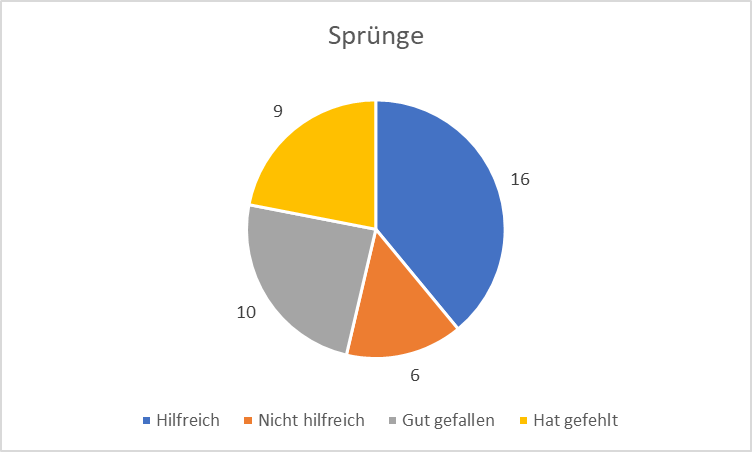
\includegraphics[width=\linewidth]{pictures/diagramme/aussagenspr}
      \caption{Wasser}
   \end{minipage}
   \hspace{.01\linewidth}% Abstand zwischen Bilder
   \begin{minipage}[b]{.49\linewidth} % [b] => Ausrichtung an \caption
      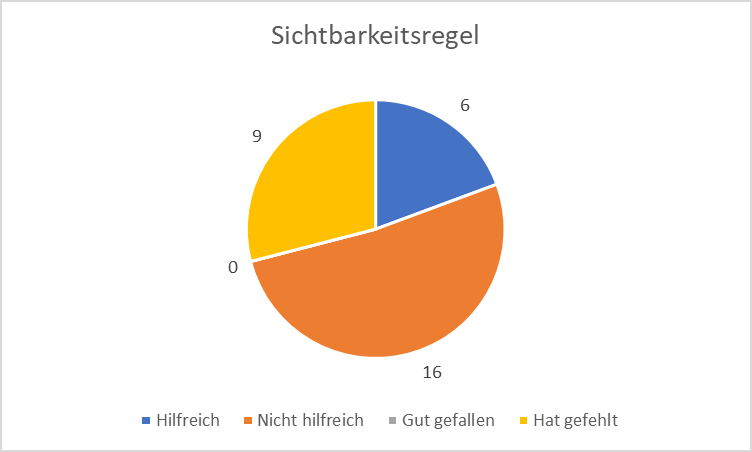
\includegraphics[width=\linewidth]{pictures/diagramme/aussagensichtb}
      \caption{Land}
   \end{minipage}
\end{figure}

\paragraph{Verständlichkeit der Konversationsdarstellung}

\paragraph{Verständlichkeit der Konversationseinstellungen}

\paragraph{Übersichtlichkeit des Konversationsverlaufs}

\paragraph{Übersichtlichkeit der Antwortoptionen innerhalb des Konversationsverlaufs}

\paragraph{Verständlichkeit der Verzweigungen innerhalb des Konversationsverlaufs}

\paragraph{Übersichtlichkeit der Werkzeugpalette zur Konversationserstellung}




\subsection{Zusammenfassung}

\section{Kritische Reflexion}

\begin{figure}[h]
\centering
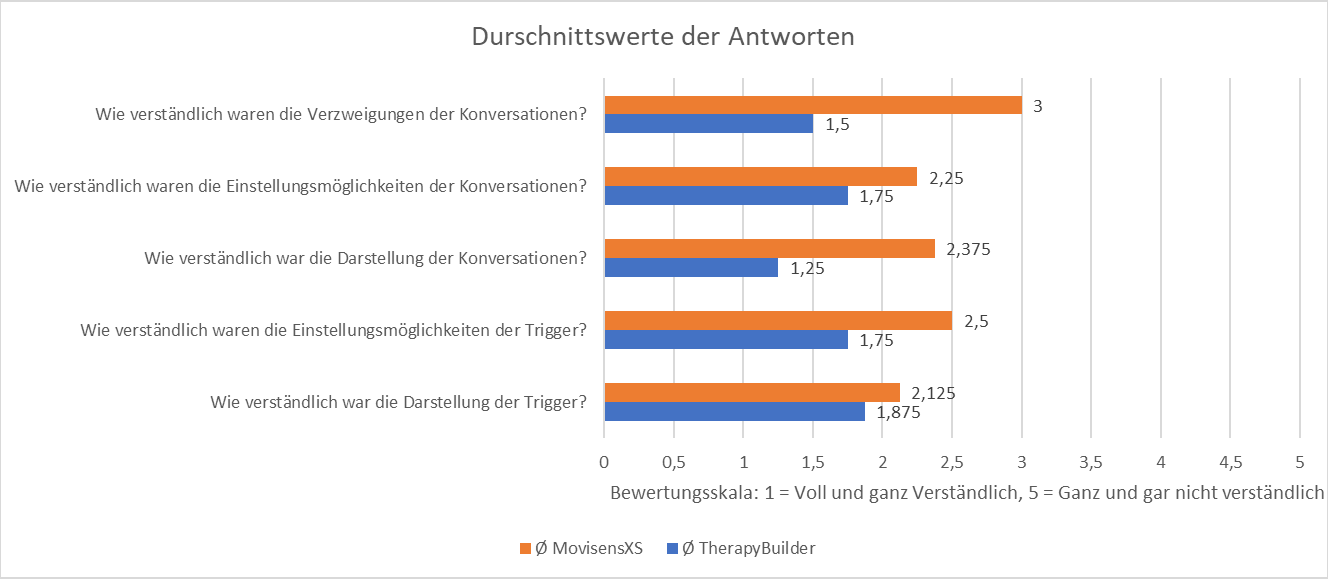
\includegraphics[width=1\textwidth]{pictures/diagramme/antwortendurchsch1}
\caption{Architektur des \emph{konfiguration}}
\label{antwortendurchsch11}
\end{figure}

\begin{figure}[h]
\centering
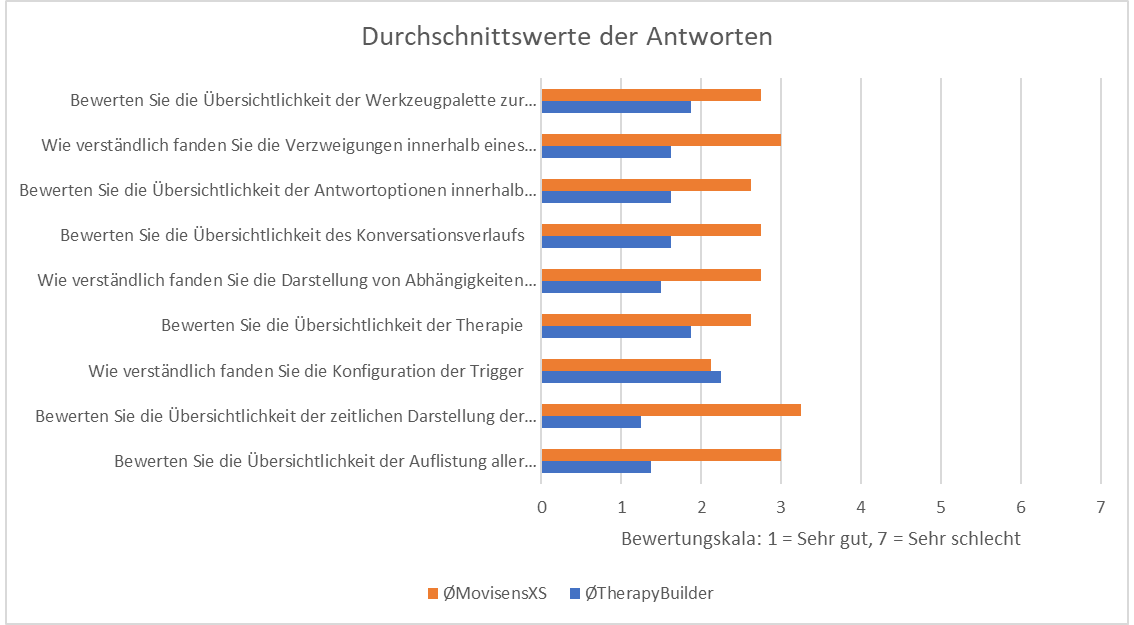
\includegraphics[width=1\textwidth]{pictures/diagramme/antwortendurchsch2}
\caption{Architektur des \emph{konfiguration}}
\label{antwortendurchsch22}
\end{figure}


%Ziel der Arbeit ist die Konzeption eines Therapiemodellierungsansatz (\emph{TMA}). Dieser soll es erlauben, auch technisch wenig versierten Psychologen ihre Therapieideen in einer Art und Weise zu formulieren, die von einer Maschine verarbeitet und ausgeführt werden kann. Dadurch entfällt der hohe und fehleranfällige Abstimmungsaufwand zwischen Forschern und Entwicklern. 


%%%%%%%%%%%%%%%%%%%%%%%%%%%%%%%%%%%%%%%%%%%%%%%%%%%%%%%%%%%%%%%%%%%%%
%%%%%%%%%%%%%%%%%%%%%%%%%%%%%%%%%%%%%%%%%%%%%%%%%%%%%%%%%%%%%%%%%%%%%

%\paragraph{Verständlichkeit der Triggerdarstellung}
%Die im Konfigurationsprinzip verwendete grafische Abbildung der zeitlichen Abläufe, durch Zeitstrahl, farbliche Kodierung, Symbole und Anordnung der Konversationen als Liste verdeutlicht, wirken sich positiv auf die Verständlichkeit der Triggerdarstellung aus. 
%
%Im Vergleich steht das Konstruktionsprinzip, welches die Triggerdarstellung als zeitliche Abläufe grafisch, als Baum und durch die Anordnung von Blöcken, wie Konversationen (Conversations), Auslösern (Triggern) und Bedingungen (Conditions) sowie einer farblicher Kodierung, nach dem Ampelprinzip, und Formen umsetzt.
%
%
%\paragraph{Verständlichkeit der Triggereinstellungen}
%Die direkte Bindung von Bedingungen (Conditions) und Auslösern (Triggern) sowie deren Einstellungen an eine Konversation wirkt sich positiv auf die Verständlichkeit der Triggereinstellungen aus. 
%
%Dem entgegen steht die Anordnung von Auslösern (Triggern) und Bedingungen (Conditions) in Verschachtelungen, mit beliebig vielen Bezügen zu Konversationen.
%
%\paragraph{Übersichtlichkeit der Konversationen}
%Die Darstellung aller vorhandenen Konversationen in Form einer Liste, innerhalb der zeitlichen Darstellung, trägt zur Verbesserung der Übersichtlichkeit der Verwendeten Konversationen bei.
%
%Innerhalb des Konstruktionsprinzips wird die Darstellung aller verwendeten Konversationen, im Samplingbaum in Form von \emph{Conversation}-Blöcke umgesetzt. Diese können beliebig im Baum platziert und angeordnet werden.
%
%\paragraph{Übersichtlichkeit der zeitlichen Darstellung der Konversationen}
%Die im Konfigurationsprinzip verwendete grafische Abbildung der zeitlichen Abläufe, in Form eines Zeitstrahls und durch Anordnung der Konversationen als Liste, trägt zu einer besseren Übersicht der zeitlichen Abfolge von Konversationen bei. 
%
%Im Vergleich steht das Konstruktionsprinzip, welches die zeitliche Abläufe grafisch, als Baum und durch die Anordnung von Blöcken, wie Konversationen (Conversations) und Auslösern (Triggern), umsetzt.
%
%\paragraph{Verständlichkeit der Triggerkonfiguration}
%Die Art der Unterscheidung zwischen Trigger und Condition tragen zur Verständlichkeit der Konfiguration der Triggereinstellungen einer Konversation bei. Hierbei gibt es zwischen Trigger und Condition keine Abhängigkeit. 
%
%Im Gegensatz zum Konfigurationsprinzip setzt das Konstruktionsprinzop eine Unterscheidung zwischen Trigger und Condition innerhalb des Samplingbaums ein. Diese werden durch Blöcke dargestellt, die sich in Farbe, Form und Anordnungsmöglichkeit unterscheiden. Trigger und Conditions sind außerdem voneinander abhängig.
%
%\paragraph{Übersichtlichkeit der Therapie}
%Insgesamt tragen die Verwendeten Stilmittel des Konfigurationsprinzip, zur Übersichtlichkeit einer Therapie, bei. Die Verwendeten Stilmittel sind hierbei die Auflistung der Verwendeten Konversationen, die zeitliche Darstellung dieser in einem Zeitstrahl, Unterscheidung dieser anhand von Farben und Formen sowie Verdeutlichung von Abhängigkeiten zwischen Konversationen durch Linien. 
%
%Dieser Form der Übersicht steht die Darstellung der Therapie in Form eines Baums entgegen. Die Übersicht der Therapie wird hierbei durch Anordnung der Blöcke, deren Farben sowie Inhalte, Verbindungen und Anordnung gegeben. 
%
%
%\paragraph{Verständlichkeit von Abhängigkeiten zwischen Konversationen und Konversationsverzweigungen}
%Die Abbildung der Abhängigkeiten zu anderen Konversationen im Zeitstrahl und der Verzweigung von Konversationen, visualisiert durch Linien, wirkt sich positiv auf die Verständlichkeit von Verzweigungen von Konversationen und Abhängigkeiten zwischen Konversationen aus. 
%
%Diesem Designprinzip steht die Darstellung von  Abhängigkeiten zu anderen Konversationen durch Verzweigungen im Baum und \emph{Check Variable} Blöcke entgegen. 


%%%%%%%%%%%%%%%%%%%%%%%%%%%%%%%%%%%%%%%%%%%%%%%%%%%%%%%%%%%%%%%%%%%%%
%%%%%%%%%%%%%%%%%%%%%%%%%%%%%%%%%%%%%%%%%%%%%%%%%%%%%%%%%%%%%%%%%%%%%


%\subsubsection{Sprünge und Sichtbarkeitsregeln}
%Die verwendeten Sprünge und damit einhergehende Darstellung, wird hinsichtlich dessen Verständlichkeit und Übersichtlichkeit überprüft. Aufgestellt werden Hypothesen, die auf die Darstellung und Einstellung einer Konversation eingehen. Insgesamt werden zum Konzept der Sprünge und dessen Umsetzung sechs Hypothesen aufgestellt, die eine Verbesserung gegenüber der Verwendung von Sichtbarkeitsregeln und der zugehörigen Darstellung messen sollen.
%
%\paragraph{Verständlichkeit der Konversationsdarstellung}
%Die Darstellung einer Konversation, welche mit dem Einsatz von Sprüngen einhergeht, trägt zur besseren Verständlichkeit der Konversationsdarstellung bei. In der Umsetzung werden Chatverläufe in einer Weise dargestellt, die in bekannten Chat-Technologien zum Einsatz kommt. Dies beinhaltet räumliche wie farbliche Trennung der Chatbot-Ausgaben und Nutzer-Eingaben.
%
%Dieser Form der Umsetzung wird die Unterscheidung durch Icons und Textbeschreibung entgegen gestellt.
%
%
%\paragraph{Verständlichkeit der Konversationseinstellungen}
%Das Einbauen eines Elements, welches Variablen überprüft und sich auf mehrere Elemente auswirken kann, trägt zur besseren Verständlichkeit der Einstellung des Konversationsverlaufs bei.
%
%Das Konzept der \emph{Sichtbarkeitsregeln}, welches entgegen gestellt wird, nutzt die Metapher eines Auges. Dieses kann an einer Form aktiviert werden um eine Sichtbarkeitsregel zu hinterlegen. Die Sichtbarkeitsregel bezieht sich nur auf die entsprechende Form. 
%
%\paragraph{Übersichtlichkeit des Konversationsverlaufs}
%Die Verwendung von Spalten, sogenannten \emph{Lanes}, tragen zur Übersicht von Konversationsverzweigungen bei.
%
%
%\paragraph{Übersichtlichkeit der Antwortoptionen innerhalb des Konversationsverlaufs}
%Die Visualisierung von Nutzereingabe innerhalb der Dialogansicht durch den Einsatz der Button-Metapher trägt zur besseren Übersicht der Antwortmöglichkeiten des Nutzers bei.
%
%Diesem Konzept steht die Darstellung der Antwortmöglichkeiten nach öffnen der Einstellungen einer Form entgegen.
%
%
%\paragraph{Verständlichkeit der Verzweigungen innerhalb des Konversationsverlaufs}
%Die Visualisierung von Verzweigungen innerhalb eines Dialogverlaufs mittels Bedingungsblock und Verweis auf Lanes, tragen maßgeblich zur Verständlichkeit bei. Der Nutzer versteht, dass es sich um eine Verzweigung handelt und welche Auswirkungen diese hat. 
%
%Diesem Design steht die Visualisierung von Verzweigungen innerhalb eines Dialogverlaufs mit Sichtbarkeitsregeln entgegen.



%\paragraph{Übersichtlichkeit der Werkzeugpalette zur Konversationserstellung}
%Eine strikte Trennung von Chatbot-Ausgabe und Nutzereingabe trägt maßgeblich zur Übersichtlichkeit der Werkzeugpalette bei. 
%
%Dem steht die Trennung von Chatbot-Ausgabe ohne Erwartung eines Nutzerinputs und Chatbot-Ausgaben mit Erwartung eines Nutzerinputs entgegen, die im \emph{movisensXS}-Prototyp verwendet wird. 

%Dieses Konzept wurde ebenfalls von den Probanden bewertet. Aus der Bewertung lassen sich folgende Aussagen treffen. 

%Auf Basis der Sichtbarkeitsregel und dem Design des Konversationsverlaufs wurde die Darstellung der Konversationen generell als zumeist verständlich bewertet. Es lässt sich eine leichte Tendenz erkennen, die angibt, dass die Darstellung zum Teil verständlich ist. Die Probandenaussagen der Freitexte untermauern die Bewertung. Es wurden bezüglich der Darstellung keine Punkte genannt, die den Probanden besonders positiv hervorstach. Hingegen wurden mehrere Aussagen getroffen, welche die Darstellung der Konversationen bemängeln. Etwas mehr als sechzig Prozent der Nutzer haben sich diesbezüglich negativ geäußert.

%Die Einstellungmsöglichkeiten der Konversationen wurde von den Probanden ebenfalls als zumeist verständlich, mit leichter Tendenz zu zum Teil verständlich, wahrgenommen. Hier wurde in knapp achtunddreißig Prozent der Aussagen die Vielfalt der Einstellungsmöglichkeiten positiv hervorgehoben. Auch die Kategorisierung der Einstellungsmöglichkeiten wurde einmal positiv erwähnt. Hingegen wurde ebenfalls in achtunddreißig Prozent der Aussagen die Unterscheidbarkeit zwischen Chatbot-Output und Patient-Input Elementen, innerhalb des Werkzeugkastens, bemängelt. Diese unterscheiden sich kaum. 

%Als gut, mit starker Tendenz zu eher gut, wurde im Schnitt die Übersichtlichkeit des Konversationsverlaufs bewertet. Vier der Freitextaussagen bemängeln die Übersicht der Konversationen. Zum einen sei der zeitliche sowie der generelle Verlauf schwer nachvollziehbar.

%Die Übersichtlichkeit der Antwortoptionen innerhalb eines Konversationsverlauf wurden von den Probanden im Schnitt als gut empfunden. Die durchschnittliche Bewertung weist dabei eine starke Tendenz zu \emph{eher gut} auf. Dies lässt sich auch in den schriftlichen Aussagen der Probanden wiederfinden. Vier Aussagen äußern sich negativ zur Darstellung des Verlaufs. Keine Aussage geht speziell auf die Antwortoptionen ein. 

%Als eher gut bewerteten die Probanden im Schnitt die Verständlichkeit der Verzweigungen innerhalb einer Konversation. Hierzu passen die Freitext-Aussagen der Probanden, die angaben, dass die Übersicht des zeitlichen Verlaufs fehle und somit für diese Probanden eher schwer nachvollziehbar ist. Diese Aussage trafen fünfzig Prozent. Ein Proband wies außerdem darauf hin, dass ihm unklar ist, woher die Variable stammt, die für die Verzweigung überprüft wird. 

%Im Schnitt bewerteten die Probanden die Übersichtlichkeit der Werkzeugpalette zur Erstellung des Konversationsverlaufs als gut. Auch hier zeigte sich eine starke Tendenz zur schlechteren Bewertung. Hier merkte ein Probanden an, dass der Zustand der Werkzeugpalette beim Öffnen des Konversationsreiters, hinderlich ist. Die Einstellungsmöglichkeiten des Chatbot-Outputs sind durch diesen leicht zu übersehen. 	%Ergebnisse
%% zusammenf.tex
%% $Id: zusammenf.tex 4 2005-10-10 20:51:21Z bless $
%%

\chapter{Ausblick}
\label{ch:FutureWork}
%% ==============================
%

Die Ergebnisse der Studie weißen auf verschiedene, erste Verbesserungsmöglichkeiten der Ansätze hin. Zur weiteren Untersuchung der Ergebnisse, werden noch zwei weitere Probanden untersucht. Anschließend werden alle Aufnahmen transkribiert und auf weitere Aussagen untersucht. Auch werden die Zeiten der Aufgabenbearbeitung in die Evaluiation mit einbezogen und anschließend die Ergebnisse neu diskutiert. Die daraus resultierenden Ergebnisse werden im Anschluss eingearbeitet und in einem ersten Programmatischen Entwurf in der Forscher-Plattform des \emph{TherapyBuilders} umgesetzt. Auch das \emph{movisensXS}-System wird anhand der Ergebnisse angepasst. Die Systeme werden erneut evaluiert. Für die Evaluation wird die, im Rahmen dieser Masterarbeit, beschriebenen Studie hinsichtlich ihrer Defizite verbessert und erneut, mit einer größeren Probandengruppe, durchgeführt. Angepasst wird die Studie hinsichtlich der Fragestellungen des Studienleiters. Die Ergebnisse der Studie werden anschließend verwendet um eine erste produktive Version der Forscher-Plattform des \emph{TherapyBuilders} zu veröffentlichen.  % Ausblick

%% ++++++++++++++++++++++++++++++++++++++++++
%% Anhang
%% ++++++++++++++++++++++++++++++++++++++++++

\appendix
%\include{anhang_a}
%\include{anhang_b}

%% ++++++++++++++++++++++++++++++++++++++++++
%% Literatur
%% ++++++++++++++++++++++++++++++++++++++++++
%  mit dem Befehl \nocite werden auch nicht 
%  zitierte Referenzen abgedruckt
\cleardoublepage
\phantomsection
\addcontentsline{toc}{chapter}{\bibname}
%%
%\nocite{*} % nur angeben, wenn auch nicht im Text zitierte Quellen 
           % erscheinen sollen
%\bibliographystyle{itmabbrv} % mit abgekürzten Vornamen der Autoren
%\bibliographystyle{gerplain} % abbrvnat unsrtnat
% spezielle Zitierstile: Labels mit vier Buchstaben und Jahreszahl
%\bibliographystyle{itmalpha}  % ausgeschriebene Vornamen der Autoren
\printbibliography
%% ++++++++++++++++++++++++++++++++++++++++++
%% Index
%% ++++++++++++++++++++++++++++++++++++++++++
\ifnotdraft{
\cleardoublepage
\phantomsection
\printindex            % Index, Stichwortverzeichnis
}
\end{document}
%% end of file

